\documentclass{/home/daniel/GitHub/USC-Physics-Degree-Notes/Notes/Apuntes}
\addbibresource{sample.bib} % si quieres incluir la bibliografía

% Autor y título

\author{Daniel Vazquez Lago}
\title{Notas Física del estado sólido}

\begin{document}
\pagenumbering{gobble} % Desactiva la numeración de páginas
% Aquí metes portada, dedicatoria...
\begin{titlepage}
\begin{tikzpicture}[remember picture, overlay]
\node[anchor=north west, inner sep=0] at (current page.north west) {%
	\includegraphics[width=\paperwidth,height=\paperheight]{../Portadas/Diseño_01_EF.png}%
	};
\end{tikzpicture}
\begin{textblock*}{4cm}(15.5cm,26cm) % Tamaño de la imagen (4cm) y posición (0cm desde el borde izquierdo, 24cm desde el borde inferior)
	
\includegraphics[scale=0.07]{../Portadas/USC_inv.png}%
\end{textblock*}
\end{titlepage}	

\newpage

\cleardoublepage
\pagenumbering{Roman} % Activas números romanos mayúsculos (I, II, III)

\addcontentsline{toc}{chapter}{Índice general}
\tableofcontents 
\newpage

\setlength{\parskip}{1.8mm} % Cambia el espacio entre párrafos

\prefacio 

\cleardoublepage
\pagenumbering{arabic} % Cambias a arábigos (1, 2, 3...)
\mainmatter % Habilitas numeración de capítulos

\chapter{Física de semiconductores}

\section{Banda de valencia y conducción}

Un semiconductor es un material sólido que presenta dos bandas (en realidad presenta más, solo accesibles\footnote{Cuando decimos accesibles nos referimos a que existe una posibilidad no nula de que estén ocupadas.} a energías térmicas o electromagnéticas muy altas, y por tanto innecsarias para nuestro estudio). Para definir una banda primero tenemos que entender que los electrones en los sólidos se pueden describir mediante una suma de ondas planas, y por tanto la energía de estos se puede describir como una función del momento dse onda $E(k)$ (aunque no tiene porque ser necesariamente de la forma $E=\hbar^2 k^2/2m$). Así, debido al caracter fermiónico de los electrones y otros potenciales aparecen energías inaccesibles para nuestros electrones, i.e. para ningún $k$ existen esas energías. Así aparecen diferentes \textit{bandas}, limitadas por una \textit{energía superior} y una \textit{energía inferior}. 

\begin{figure}[h!] \centering
	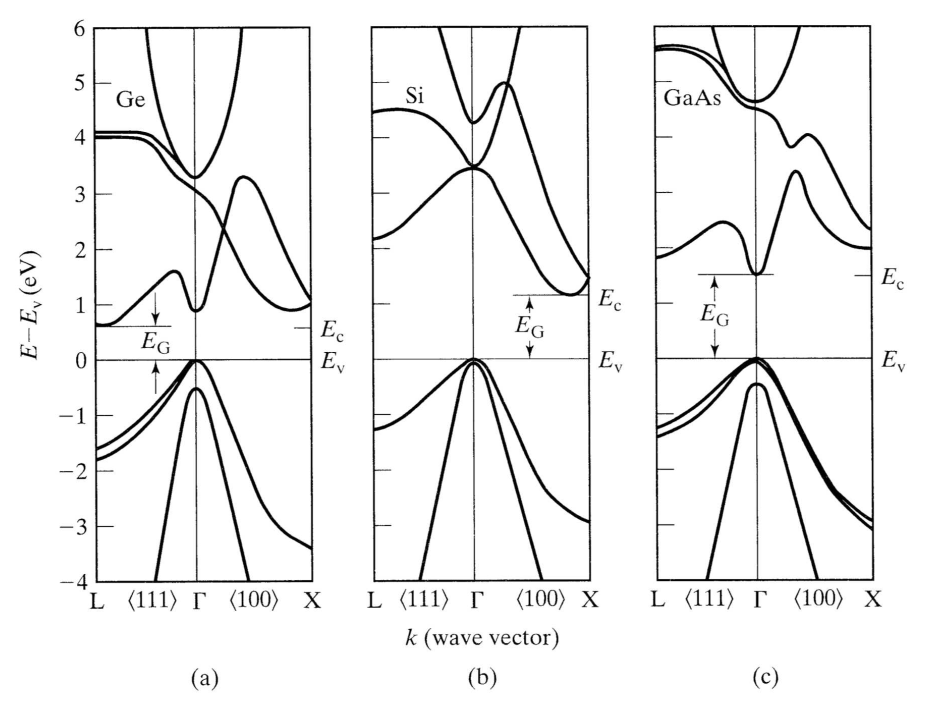
\includegraphics[width=0.7\textwidth]{Cuerpo/Ch_01/01_01.png}
	\caption{Bandas de conducción y valencia para algunos semicdonductores.}
\end{figure}

Como dijimos, un semiconductor posee dos bandas, separadas por una energía $E_g$. A la banda con energía superior se le llama \textbf{banda de conducción} (B.C) y a la banda inferior se le llama \textbf{banda de valencia} (B.V). Las bandas, a su vez, poseen diferentes líneas de dispersión, esto es diferentes relaciones $E(k)$. El número y forma de estas dependerá del tipo de material y la dirección de la onda, por esa misma razón solemos ver en la parte inferior de las bandas $\langle 111\rangle $ o $\langle 100\rangle$. Está denotando la dirección de la onda. En general suelen ser materiales muy simétricos, y por tanto con pocas direcciones representamos todas las posibles relacioens de dispersión. 

La \textit{energía mínima de la banda de conducción} se denota como $E_c$, la \textit{energía máxima de la banda de valencia} se denota por $E_v$, y la diferencia entre el máximo de la BV y el mínimo de BC se denota por $E_g$:

\begin{equation}
	E_g = E_c - E_v
\end{equation}
En general se suele definir $E_v=0$ como referencia. Así la banda de valencia posee energías negativas, y la banda de conducción energías positivas. Veamos las características de las bandas:

\begin{itemize}
	\item \textbf{Banda de valencia:} el \textit{máximo siempre aparece en $k=0$}. Está dividida en 3 subbandas (3 relaciones de dispersión), 2 de ellas degeneradas en $k=0$ (son indistiguibles en $k=0$). 
	\item \textbf{Banda de conducción:} está dividida en subbandas (aunque el número depende del material), y el valor de $k_{\min}$ tal que $E_{\min}=E(k_{\min})$ del dependerá del material. 
\end{itemize}


\subsection{Semiconductores directos e indirectos}

Como hemos dicho, $E_c$ es el mínimo de la banda de conducción y $E_v$ es el máximo de la banda de valencia. En función del valor de $k_{\min}$ distinguimos dos tipos de semiconductores:
\begin{itemize}
	\item Definimos un \textbf{semiconductor indirecto} a aquel que verifica que $k_{\min}\neq0$. Es decir, el gap de energía sucede entre diferentes momentos (lo que hará que cuando se excite a un electrón de la BV tenga que darsele un momento).
	\item Definimos un \textbf{semiconductor directo} a aquel que verifica que $k_{\min}=0$. Es decir, el gap de energía sucede a $\Delta k =0$ (lo que hará que cuando se excite a un electrón de la BV no se pueda intercambiar momento).
\end{itemize}


\begin{figure}[h!] \centering
	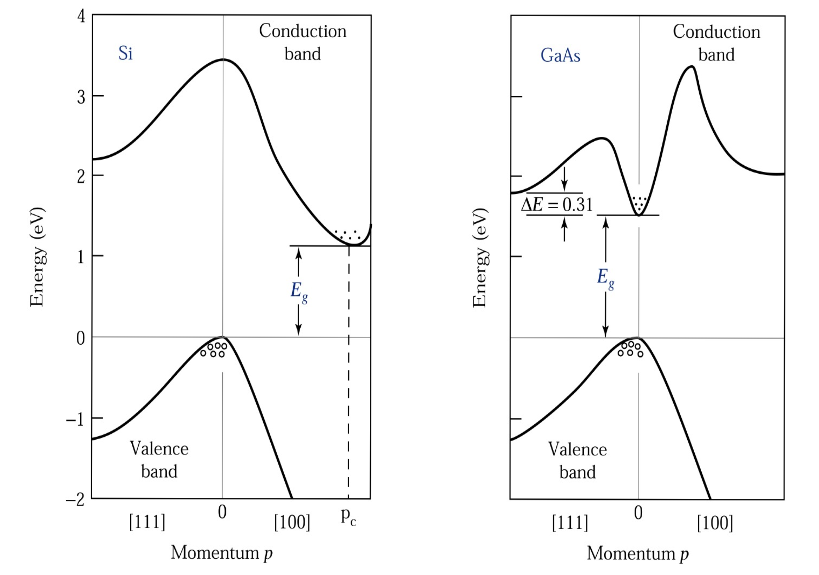
\includegraphics[width=0.8\textwidth]{Cuerpo/Ch_01/01_02.png}
	\caption{Bandas de conducción y valencia para algunos semicdonductores.}
\end{figure}


\subsection{Forma de los mínimos y máximos de banda: masa equivalente}

Cerca de los extremos de las bandas $E_0=E(k_0)$ tenemos que se puede aproximar la enerǵia por una función parabólica, tal que:

\begin{equation}
	E = E_0 + \frac{1}{2} \parentesis{\parciales{^2E}{k^2}}_{k_0} (k-k_0)^2 
\end{equation}
Como podemos ver, esto se parece mucho a la expresión $E=\hbar^2k^2/2m$ que se usa para \textit{partículas libres}. Es decir, cerca de los extremos de las bandas, los \textit{portadores actúan como partículas libres con masa efectiva $m^*$} definida como

\begin{equation}
	(m^*)^{-1} = \frac{1}{\hbar^2} \parciales{^2E}{k^2} 
\end{equation}

\begin{Anotacion}
	\textcolor{red}{Imagen de los mínimos/máximos.}
\end{Anotacion}

\subsection{Ecuación del movimiento}

La ecuación del movimiento para los electrones es una generalización de la ecuación de Newton usando el momento de onda del electrón $\kn$. Sabiendo que 

\begin{equation}
	\Fn = m^* \an = m^* \dot{\vn} = m^* \hbar \dot{\kn}{m^*} 
\end{equation}
de lo que se deduce que 

\begin{equation}
	\hbar \derivadas{\kn}{t} = \Fn
\end{equation}
pudiendo ser la fuerza, por ejemplo, la fuerza de Lorentz $\Fn=-e(\En+\vn \times \Bn)$, o cualquier otra.

%%%%%%%%%%%%%%%%%%%%%%%%%%%%%%%%%%%%%%%%%%%%%%%%%%%%%%%%%%%%%%%%%%%%%%%
%%%%%%%%%%%%%%%%%%%%%%%%  SECCIÓN 2 %%%%%%%%%%%%%%%%%%%%%%%%%%%%%%%%%%%
%%%%%%%%%%%%%%%%%%%%%%%%%%%%%%%%%%%%%%%%%%%%%%%%%%%%%%%%%%%%%%%%%%%%%%%
\section{Portadores: conecpto de hueco y electrón}

En los semiconductores hay 2 tipos de portadores, los portadores tipo hueco (o tipo $p$\footnote{Por el hecho de que se pueden describir como partículas con carga positiva.}) y tipo electrón (tipo $n$). La pregunta que nos deberíamos plantear en este momento es: ¿Qué sentido tiene que existan portadores tipo electrón/hueco si solo tenemos electrones en el semiconductor?¿Como que tipo electrón, no deberían ser electrones? La respuesta como siempre es complicada. Como hemos dicho, cerca de los extremos las partículas, los electrones se comportan como electrones libres con masa efectiva $m^*$ (de hay viene \textit{tipo electrón} se comportan casí como electrones). Sin embargo, esto lleva a un problema, ya que la masa efectiva de un electrón en el máximo de la banda de valencia sea negativa (en un máximo $\partial^2 E/ \partial k^2<0$), 

Supongamos que tenemos la capa de valencia llena salvo por un electrón, que se ha excitado y ha subido a la capa de conducción. En la banda de valencia habrá entonces $N$ electrones menos uno. La suma de los momentos de todos los electrones de la banda será entonces:

\begin{equation}
	\kn = \sum_{i=1}^{4N-1} \kn_i 
\end{equation}
o lo que es lo mismo:

\begin{equation}
	\kn = \sum_{i=1}^{4N} (\kn_i) - \kn_e
\end{equation}
denotándolo por $\kn_e$ ya que es un electrón cualquiera (son indistiguibles). Como sabemos, la suma del momento de los electrones en una banda tiene que ser cero, ya que $k$ tiene tanto valores negativos y positivas, y están todos ocupados. Es decir, tenemos que el momento total de la banda será:

\begin{equation}
	\kn \equiv \kn_h = - \kn_e
\end{equation}
si a este momento total lo llamamos $\kn_p$ (momento de portador $p$ o hueco), tenemos que \textit{el movimiento efectivo de una capa sin un electrón es en el sentido opuesto al que tendría un electŕon individual en la misma}. A este artificio matemático lo llamamos hueco, y no es más que la manera de describir el comportamiento de una capa entera a través de unas pocas partículas. La energía también tendrá el signo opuesto, ya que:

\begin{equation}
	E_h = \sum_{i} E_i - E_e 
\end{equation}
y como $\sum_{i}E_i$ es una constante (se define como cero). Así pues:

\begin{equation}
	E_h \equiv - E_e
\end{equation}
Y por tanto, aunque la masa efectiva de un electrón en el máximo de la banda de valencia sea negativa (en un máximo $\partial^2 E/ \partial k^2<0$), para el objeto matemático así definido tenemos que la masa efectiva será positiva, y la carga será positiva. Que la carga sea positiva no es tan obvio. Para ello tenemos que ver que la ecuación del movimiento 

\begin{equation}
	\hbar \derivadas{\kn_h}{t} = -e(\En + \vn_h \times \Bn)
\end{equation}
hace que se comporte como un electrón con carga positiva $(\kn_h \equiv - \kn_e)$. La pregunta ahora es: ¿Tiene sentido físico? La respuesta es que sí. El sentido físico está en que cuando excitamos un electrón a la BC desde la BV, queda un estado sin ocupar, un hueco, en la banda de valencia. Este hueco podría ser rellenado por los electrones vecinos, que desde fuera lo veríamos como un movimiento efectivo del hueco, que además tendría el sentido contrario al del electrón (si los electrones saltan por ejemplo de izquierda a derecha por culpa de un campo eléctrico, veremos al hueco saltando de la derecha a la izquierda). 

Consecuentemente los electrones en la banda de conducción se comportarán como electrones normales libres por la salvedad de que la masa efectiva será diferente; mientras que la falta de electrones en la banda de conducción (por la excitación de estos a la banda de conducción) se describirá a través de una serie de partículas con masa efectiva positiva diferente a la masa del electrón, carga positiva, con momento y energía efectiva de signo contrario al que tendría un electrón libre en la banda de valencia.


%%%%%%%%%%%%%%%%%%%%%%%%%%%%%%%%%%%%%%%%%%%%%%%%%%%%%%%%%%%%%%%%%%%%%%%
%%%%%%%%%%%%%%%%%%%%%%%%  SECCIÓN 3 %%%%%%%%%%%%%%%%%%%%%%%%%%%%%%%%%%%
%%%%%%%%%%%%%%%%%%%%%%%%%%%%%%%%%%%%%%%%%%%%%%%%%%%%%%%%%%%%%%%%%%%%%%%

\section{Densidad de portadores y clasificación de semiconductores}

En esta sección vamos a tratar de expresar la densidad de portadores hueco, denotado por $p$, y la densidad de portadores electrones, denotado por $n$. Primero estudiaremos el caso mas general posible, en función de la densidad de estados $g(E)$ y de la función de Fermi-Dirac $f(E)$. Luego iremos haciendo ciertas aproximaciones para simplificar los resultados.

\subsection{Densidad de portadores en el caso más general posible}

El caso más general, como ya hemos dicho, estudia el número de portadores $n$ y $p$ a partir de las integrales sobre las densidades de energía y función de Fermi. La \textit{densidad de estados} $g(E)$ es la distribución de los estados de energía a una energía dada, mientras que la \textit{función de Fermi} indica, en condiciones de equlibrio, la probabilidad de que un estado permitido de enerǵia $E$ esté ocupado por un electrón. La función de densidad de estados depende de la dimensión del sistema, tal que:

\begin{equation}
	g_{3D} (E) = \frac{\sqrt{2}m^{3/2}E^{1/2}}{\pi^2 \hbar^3} \quad g_{2D} (E) = \frac{m}{\pi \hbar^2} \quad g_{1D} (E) = \frac{\sqrt{2}m^{1/2}}{\pi \hbar \sqrt{E}}
\end{equation}
La dedución de estas densidades no es exageradamente complicada, véase apéndice \ref{Sec:A-01}. Por otra parte, la función de Fermi nos dice que la probabilidad de que cierto estado esté ocupado es: 


\begin{equation}
	f(E) = \frac{1}{1+e^{(E-E_F)/kT}}
\end{equation}
donde $E_F$ es la enerǵia de Fermi, de la cual hablaremos más adelante. Naifmente uno podría pensar que la densidad $n/p$ sería simplemente la integral $g(E)f(E)$ entre diferentes intervalos de energía, ya que como sabemos los huecos se encuentran siempre en la banda de conducción, y por tanto entre las energías $E_{\min}$ y $E_c$, mientras que los huecos se encuentran en la banda de valencia, y por tanto entre las energías $E_{\max}$ y $E_v$.

Sin embargo esto no es correcto, por dos razones. La primera de ellas es que por culpa de la forma de parábola cerca del máximo y el mínimo de la banda de valencia y conducción respectivamente, es necesario redefinir el cero en el máximo local/mínimo local. La razón no es evidente a primera vista, pero uno lo puede entender cuando piensa que en un extremo local solo caben 2 electrones (uno con espín arriba y otro con espín abajo). Así pues, las densidades en la banda de valencia $g_v(E)$ y en la banda de conducción $g_c(E)$ son:

\begin{equation}
	g_c(E) = \frac{(m_n^*)^{3/2} \sqrt{2(E-E_c)}}{\pi^2 \hbar^3} \quad E \geq E_c \qquad 	g_v(E) = \frac{(m_p^*)^{3/2} \sqrt{2(E_v-E)}}{\pi^2 \hbar^3} \quad E \leq E_v
\end{equation}
La segunda razón es que si $f(E)$ es la probabilidad de que esté un estado ocupado con energía $E$ en el equilibrio, entonces $1-f(E)$ será la probabilidad de que no esté ocupado, y por tanto la probabilidad de que haya un hueco. Así pues, \textbf{las densidades de los portadores son}

\begin{equation}
	n=\int_{E_c}^{E_{\max}} g_c(E)f(E)\D E \qquad p = \int_{E_{\min}}^{E_v} g_v(E) (1-f(E))\D E
\end{equation}
que se puede aproximar para obtener las densidades en función de la llamada \textit{integral de Fermi-Dirac de orden 1/2} $F_{1/2}(\eta_c)$. La aproximación consiste básicamente en decir que $E_{\max} \rightarrow \infty$, y que por tanto

\begin{equation}
	n = \frac{1}{2\pi^2} \parentesis{\frac{2m_e^*}{\hbar^2}}^{3/2} (kT)^{3/2} F_{1/2}(\eta_c) \qquad F_{1/2}(\eta_c) = \int_0^\infty \frac{\eta^{1/2}}{1+e^{\eta-\eta_c}}\D \eta 	
\end{equation}
\begin{equation}
	\eta=\frac{E-E_c}{kT} \qquad \eta_c= \frac{E_F-E_c}{kT}
\end{equation}
(no hemos hecho todos los pasos para deducir la forma ya que no se va a usar en nigún momento).
Esta ecuación no tiene solución analítica, por tanto es necesario hacer ciertas aproximaciones si queremos trabajar con ella, lo cual trataremos en el siguiente apartado. 

\subsection{Semiconductores no degenerados y degenerados}

Como hemos dicho, las densdiades de los portadores en función de la integral de Fermi-Dirac
La aproximación más interesante es la llamada \textit{aproximación de Bolztmann}, que nos permite obtener una solución muy sencilla, que es la siguiente:

\begin{equation}
	F_{1/2} (\eta_c) = \int_{0}^{\infty} \frac{\eta^{1/2}}{1+ e^{\eta-\eta_c}} \D \eta \simeq \frac{\sqrt{\pi}}{2} e^{\eta_c} 
\end{equation}
Esta aproximación solo es válida cuando $E_c-3kT>E_F>E_v+3kT$, y por tanto cuanta más alta la temperatura más restringida será su aplicación. Cuando un semiconductor verifica estas condiciones para una temperatura dada decimos que se encuentra en el \textit{régimen no degenerado}, mientras que cuando \textit{no} verifica dichas condiciones decimos que está en el \textit{régimen degenerado}.

\begin{figure}[h!] \centering
	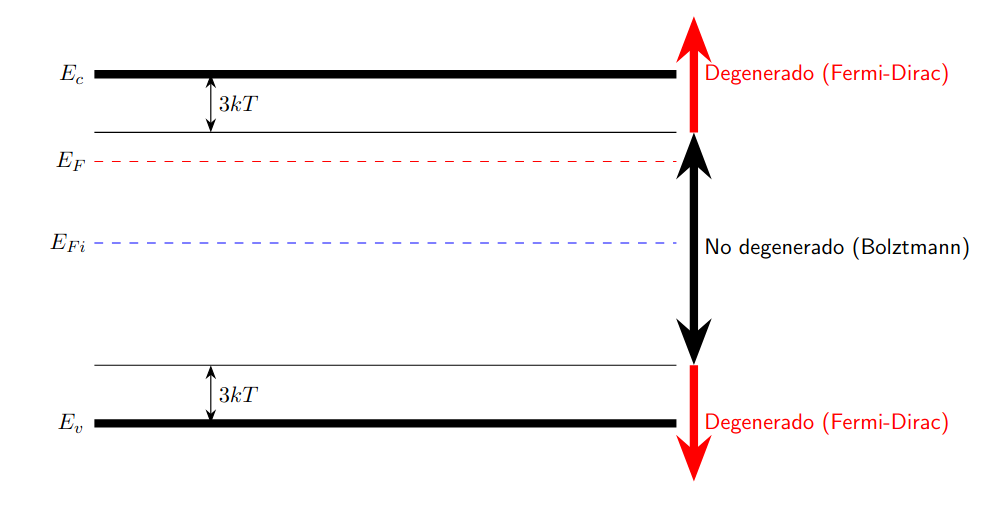
\includegraphics[width=0.85\textwidth]{Cuerpo/Ch_01/01_03.png}
	\caption{Régimen degenerado y no degenerado.}
\end{figure}


En general nosotros trabajaremos únicamente con semiconductores no degenerados, y por tanto en el rango de validez de la aproximación de Bolztmann, la que da como resultado las siguientes densidades de portadores:

\begin{equation}
	p=N_v e^{(E_v-E_F)/kT}  \qquad n = N_c e^{(E_F-E_c)/kT}
\end{equation}
donde $N_c$ y $N_v$ son las llamadas \textbf{densidades equivalentes de los estados de la banda de valencia y conducción}, con la siguiente forma:

\begin{equation}
	N_c = 2 \parentesis{\frac{m_n^* kT}{2\pi\hbar^2}}^{3/2} \tquad 
	N_v = 2 \parentesis{\frac{m_p^* kT}{2\pi\hbar^2}}^{3/2}
\end{equation}
Para una temperatura aproximada de $300$K tenemos que 

\begin{equation}
	N_{C,V} = (2.509\times10^{19} \cm^{-3}) \parentesis{\frac{m_{n,p}^*}{m_0}}^{3/2}
\end{equation}
siendo $m_0$ la masa del electrón.
\subsection{Semiconductores intrínsecos caso no degenerado}

Definimos como \textbf{semiconductor intrínseco} a un material semiconductor extremadamente puro, sin dopantes, cuyas propiedades solo dependan del material. En este tipo de materiales el número de electrones es igual al número de huecos (en virtud de la neutralidad electrónica: el número de electrones en la banda de conducción será el mismo el número que electrones faltan en la banda de valencia, i.e. el número de huecos). Matemáticamente se expresa como 

\begin{equation}
	n = p = n_i
\end{equation}
y se llama \textit{condición intrínseca}. Siempre que estudiemos semiconductores intrínsecos lo haremos a través de los semiconductores no degenerados, ya que de cualquier otra forma no podemos tener expresiones analíticas. Denotamos $E_i$ al \textbf{nivel de fermi intrínseco}. Usando la ecuación anterior, obtenemos que:

\begin{equation}
	n_i = \sqrt{np} = \sqrt{N_CN_V} e^{-E_g/2kT} = 
\end{equation}
donde $E_g=E_c-E_v$ y se le llama \textit{energía de gap}. El valor de $n_i$ para un semicdonductor dado es muy importante, incluso cuando está dopado. La razón es que siempre podemos expresar $n$ y $p$  en función de $n_i$ (a la misma temperatura), ya que si $n=p=n_i$:

\begin{equation*}
	n_i = N_C e^{(E_i-E_c)/kT} = N_V e^{(E_v-E_i)/kT}  \Rightarrow 
\end{equation*}
\begin{equation}	
	N_C=n_i e^{(E_c-E_i)/kT} \quad N_V = n_i e^{(E_i-E_v)/kT} \label{Ec:01-3-13}
 \end{equation}
tal que
\begin{equation}
	n=n_i e^{(E_F-E_i)/kT} \qquad p = n_i e^{(E_i-E_F)/kT} \label{Ec:01-3-14}
\end{equation}
lo cual nos está dando en realidad una información muy relevante: en función del nivel de fermi, i.e., si $E_F>E_i$ o $E_F<E_i$, podremos saber si el conductor es de tipo $n$ o tipo $p$ (solo cuando $E_F=E_i$ tenemos $n=p$, precisamente la condición intrínseca). Además tenemos que de la expresión anterior podemos deducir la llamada \textbf{ley de acción de masas} (que se verifique siempre que estemos en el rango no degenerado):

\begin{equation}
	np=n_i^2
\end{equation}
Si nos damos cuenta a partir de las ecuaciones \ref{Ec:01-3-13} podemos deducir una \textit{expresión para la posición del nivel de Fermi intrínseco $E_i$}. Para esto partimos de las ecuaciones \ref{Ec:01-3-14}, de lo que se deduce que:

\begin{equation}
	E_i = \frac{E_c+E_v}{2} + \frac{kT}{2} \ln \parentesis{\frac{N_C}{N_V}} = \frac{E_c+E_v}{2} + \frac{3}{4} kT \ln \parentesis{\frac{m_p^*}{m_n^*}}
\end{equation}
Incluso podemos obtener la \textit{expresión para la posición del nivel de Fermi $E_F$} para el caso más general. Para esto partimos de las ecuaciones

\begin{equation}
	\ln \parentesis{\frac{n}{n_i}} = \frac{1}{kT} \parentesis{E_F-E_i} \Rightarrow E_F = E_i + kT \ln \parentesis{\frac{n}{n_i}}
\end{equation}
\begin{equation}
	\ln \parentesis{\frac{p}{n_i}} = \frac{1}{kT} \parentesis{E_i-E_F} \Rightarrow E_F = E_i - kT \ln \parentesis{\frac{p}{n_i}}
\end{equation}
Siendo expresiones completamente compatibles (si se verifica una se verifica la otra) además de que mantienen la relación citada antes entre el nivel de Fermi y el número de portadores huecos/electrón.

\subsection{Semiconductores extrínsecos caso no degenerado}

Definimos como \textbf{semiconductor extrínseco} o \textbf{semiconductor dopado} a un material semiconductor al que se le han insertado átomos de otro grupo. Pero antes es importante preguntarse por qué se incluyen estos átomos en nuestro semiconductor, y cuáles son sus ventajas. La respuesta todavía no podemos darla de manera muy profunda, sin embargo si podemos decir lo siguiente: a temperaturas ambiente, la cantidad de portadores tipo $n$ y tipo $p$ intrínsecas son muy bajas, y por tanto habrá una conductividad muy baja. Cuando dopamos un semiconductor no solo estamos aumentando el número de portadores de un tipo, estamos aumentando la conductividad. De hecho, al ser capaces de controlar el nivel de dopado, podemos elegir la conductividad arbitrariamente, pudiendo optimizar y controlar totalmente las propiedades eléctricas.

Así pues, tenemos dos tipos de dopantes, que además definiran el tipo de portador mayoritario que tendremos. Tenemos pues:

\begin{itemize}
	\item \textbf{Dopante dador}. Los dopantes dadores o dadores aportan electrones a la banda de conducción (por lo general son elementos del grupo V, aportando un electrón), lo que hará que el portador mayoritario sea el portador $n$. A la concentración de dadores la denotamos por $N_D$.
	\item \textbf{Dopante aceptor}. Los dopantes aceptores o aceptores aportan heucos a la banda de valencia (por lo general son elementos del grupo III, aportando un hueco), lo que hará que el portador mayoritario sea el portador $p$. A la concentración de dadores la denotamos por $N_A$.
\end{itemize}

\begin{figure}[h!] \centering
	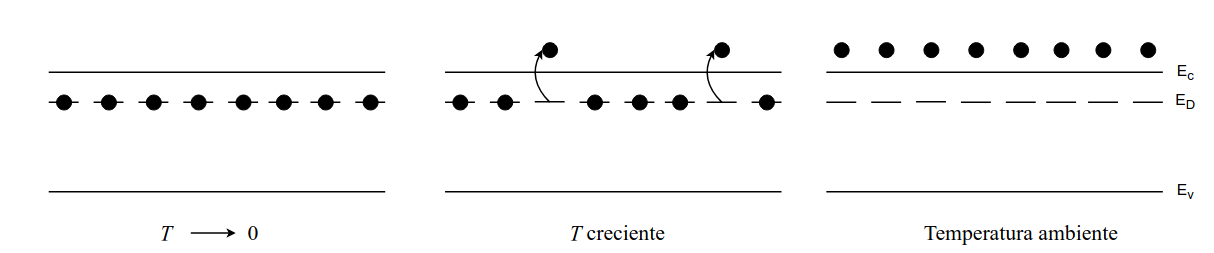
\includegraphics[width=0.9\textwidth]{Cuerpo/Ch_01/01_04.png}
	\caption{Funcionamiento de los conductores tipo $n$.}
\end{figure}

\begin{figure}[h!] \centering
	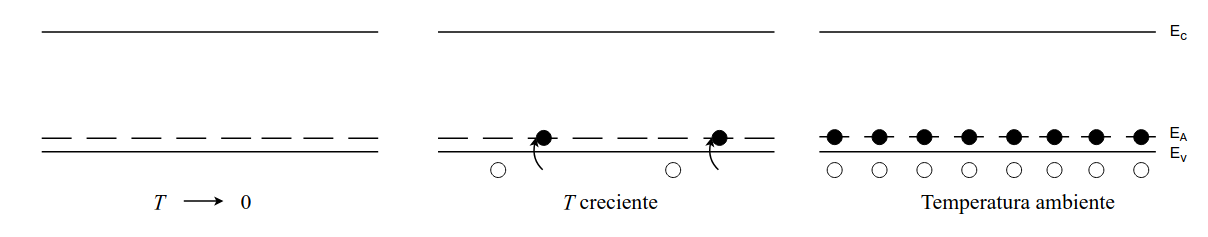
\includegraphics[width=0.9\textwidth]{Cuerpo/Ch_01/01_05.png}
	\caption{Funcionamiento de los conductores tipo $p$.}
\end{figure}

Sin embargo no es igual el número de impurezas $N_D$ y $N_A$ al número de portadores que aportan $N_D^+$ y $N_A^-$. Pensemos por ejemplo el caso de los elementos del grupo V. Para que puedan aportar el quinto electrón es necesario romper el enlace que lo une con dicho átomo, es decir, hace falta ionizarlo, lo que se hace a través de la aportación de energía, por ejemplo energía térmica. A partir de cierta temperatura todas las impurezas están ionizadas (temperatura ambiente). Sin embargo no siempre será así, y si la energía térmica no es suficiente para ionizar todas las impurezas, debemos usar las siguientes expresiones:

\begin{equation}
	N_D^+ = \frac{N_D}{1+g_D e^{(E_F-E_D)/kT}} \tquad
	N_A^- = \frac{N_A}{1+g_D e^{(E_A-E_F)/kT}} 
\end{equation}
donde $E_D$ y $E_A$ son las correspondientes energías de ionización. Al igual que antes tenemos la condición de electroneutralidad, aunque ahora va a cambiar un poco: tenemos que considerar que $N_D^+$ y $N_A^-$ aportan carga. Así pues, la \textbf{condición de electroneutralidad para extrínsecos} es:

\begin{equation}
	p + N_D^+ = n + N_A^-
\end{equation}
lo cual tiene todo el sentido del mundo: si tenemos $N_D^+>N_A^-$ (mas dadores que aceptores) lógicamente habrá más portadores tipo $n$ que tipo $p$. Dado que la ley de acción de masas $np=n_i^2$ se cumple \textit{para cualquier semiconductor no degenerado}, para cualquier conductor no degenerado extrínseco podemos conocer $n$ y $p$ en función de $n_i,N_D^+$ y $N_A^-$ (que surge tras despejar una ecuación de segundo grado):

\begin{equation}
	n = \frac{N_D-N_A}{2} + \ccorchetes{\parentesis{\frac{N_D-N_A}{2}}^2 + n_i^2}^{1/2} \tquad p = \frac{N_A-N_D}{2} + \ccorchetes{\parentesis{\frac{N_A-N_D}{2}}^2 + n_i^2}^{1/2}
\end{equation}
Los 3 casos más sencillos que nos pueden plantear son los siguientes:

\begin{itemize}
	\item Cuando $N_D^+=N_A^-$ tenemos que
	 \begin{equation}
		n=p=n_i
	\end{equation}
	\item Cuando $N_D^+ \gg N_A^-,n_i$. En este caso tenemos las siguientes ecuaciones:
	\begin{equation}
		n=N_D^+ \tquad p = \frac{n_i^2}{N_D^+}
	\end{equation}
	\item Cuando $N_A^-\gg N_D^+,n_i$. En este caso tenemos las siguientes ecuaciones:
	\begin{equation}
		p=N_A^- \tquad n = \frac{n_i^2}{N_A^-}
	\end{equation}
\end{itemize}
El resto de casos habrá que calcularlos aparte. 

\subsection{Semiconductores extrínsecos: régimen intrínseco y extríseco}

Definimos como \textbf{régimen extrínseco} de un semiconductor extrínseco\footnote{Muchas veces, cuando se dice que está en el semicdonductor está en el régimen extrínseco ya se asume que está dopado, y por tanto se obvia.} aquel intervalo de temperaturas (aunque puede ser otra variable) en el que todas las impurezas están ionizadas y se verifica que $N_D^+$ o $N_A^-$ es mucho mayor que $n_i$. Definimos como \textbf{régimen intrínseco} aquella región de temperaturas en la cual el nivel de impurezas excitadas es comparable o menor al número de portadores excitados por fluctuaciones térmicas $n_i$. Cuando la temperatura es baja y no están excitados todas las impurezas, decimos que estamos en el régimen de \textit{freeze out}.

Definimos como \textbf{temperatura intríseca} a la temperatura que separa el régimen extrínseco e intrínseco, y se define como aquella temperatura para la cual $n(T_i)=2N_D$ o $p(T_i)=2N_A$ en función de si es dador o aceptor el dopante. 


\begin{figure}[h!] \centering
	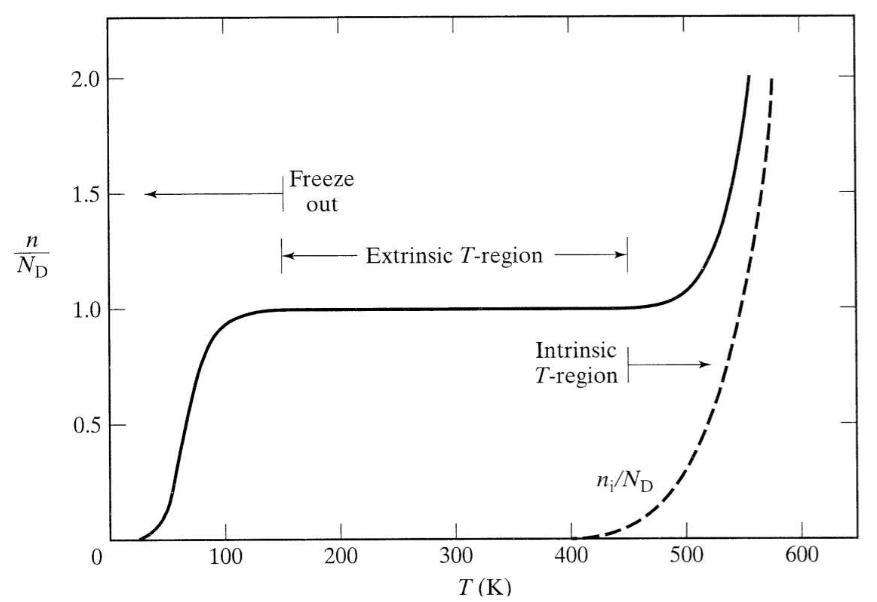
\includegraphics[width=0.85\textwidth]{Cuerpo/Ch_01/01_06.png}
	\caption{Régimenes intrínsecos y extrínsecos en función de la temperatura.}
\end{figure}


%%%%%%%%%%%%%%%%%%%%%%%%%%%%%%%%%%%%%%%%%%%%%%%%%%%%%%%%%%%%%%%%%%%%%%%
%%%%%%%%%%%%%%%%%%%%%%%%  SECCIÓN 4 %%%%%%%%%%%%%%%%%%%%%%%%%%%%%%%%%%%
%%%%%%%%%%%%%%%%%%%%%%%%%%%%%%%%%%%%%%%%%%%%%%%%%%%%%%%%%%%%%%%%%%%%%%%

\section{Valores típicos}





%%%%%%%%%%%%%%%%%%%%%%%%%%%%%%%%%%%%%%%%%%%%%%%%%%%%%%%%%%%%%%%%%%%%%%%
%%%%%%%%%%%%%%%%%%%%%%%%  EJERCICIOS %%%%%%%%%%%%%%%%%%%%%%%%%%%%%%%%%%%
%%%%%%%%%%%%%%%%%%%%%%%%%%%%%%%%%%%%%%%%%%%%%%%%%%%%%%%%%%%%%%%%%%%%%%%

\section{Ejercicios}

\tcbstartrecording

\begin{texercise}
	Se dopa silicio con Boro (B) en una proporción de 2 ppm (partes por millón)
	\begin{enumerate}[label=\alph*)]
		\item Calcula la concentración intrínseca del Si y obten una expresión de dicha concentración en función de la temperatura.
		\item Indica el tipo de conducción de este material y calcula la concentración de impurezas y la de electrones y huecos (n y p) a temperatura ambiente si todos los dopantes están ionizados.
		\item Calcula la posición del nivel de Fermi y dibuja el diagrama de bandas completo correspondiente.
		\item ¿Qué pasa si la concentración de impurezas igualase el valor de \( N_V \)? Representa gráficamente las bandas de energía frente a la concentración de impurezas usando todas las aproximaciones que conozcas.
	\end{enumerate}
	(DATO: Constante de red del Si \( a_0 = 5.431 \) Å).

	\tcblower
	Veamos las soluciones por apartados
	\begin{enumerate}[label=\alph*)]
		\item La concentración intrínseca del Silicio en un semiconductor es el número de portadores $n_i$ en el semiconductor, si no estuviera dopado. No hay que confundir la concentración intrínseca $n_i$ con la concentración $n$, en la que si se tendrá en cuenta que el material está dopado. La concentración intrínseca es:
		
		\begin{equation}
			n_i = \sqrt{N_cN_v} e^{-E_G/2kT}
		\end{equation}
		donde $E_G=E_c-E-v$, y además

		\begin{equation}
			N_{C,V} = 2 \parentesis{\frac{m_{e,p}^* kT}{2\pi\hbar^2}}^{-3/2}
		\end{equation}
		Las masass $m_p^*= 1.18m_e$ y $m_n^*=0.81m_e$. Si queremos dar el valor:

		\begin{equation}
			N_c = 3.22 \cdot 10^{19} \cm^{-3} \tquad 	N_v = 1.83 \cdot 10^{19} \cm^{-3}
		\end{equation}
		De lo que se deduce

		\begin{equation}
			n_i = 9.56 \cdot 10^9 \cm^{-3}
		\end{equation}


		\item Están dopando con boro, que es del grupo III, y por tanto es un dador. Esto significa que será un conductor tipo $p$. Para calcular la concentración de impurezas, primero tenemos que obtener la densidad de Boro en nuestro silicio. La densidad del silicio se calcular a partir de la constante de red y sabiendo que posee una red diamante. Así pues:
		\begin{equation}
			N_{Si} = \frac{8}{a_0^3} 
		\end{equation}
		de lo que se puede deducir entonces que:
		\begin{equation}
			N_B = 2\cdot 10^{-6} \cdot N_{Si} = 9.988 \cdot 10^16 \cm^{-3}
		\end{equation}
		Nos dicen que todos los dopantes están ionizados, es decir, que estamos en el régimen extrínseco. En este régimen todos los átomos de Boro son impurezas, tal que $N_A^-=N_A=N_B$. Suponiendo que $N_A^- \gg N_D^+$, tenemos que la ecuación de neutralidad de carga:

		\begin{equation}
			n\cdot p = n_i^2 \tquad p-n-N_A = 0 
		\end{equation}
		usando estas ecuaciones para despejar el valor de $n$ y $p$, tenemos que:	
		\begin{equation}
			p = \frac{N_A}{2} + \ccorchetes{\parentesis{\frac{N_A}{2}}^2 + n_i^2}^{1/2} 
		\end{equation}
		y luego calculamos 

		\begin{equation}
			n = \frac{n_i^2}{p}
		\end{equation}
		Numéricamente podemos obtener los resultados:

		\begin{equation}
			n=915.034 \cm^{-3} \quad p = 9.988 \cdot 10^{16} \cm^3
		\end{equation}


		\item La posición del nivel de Fermi de un semiconductor dopado se calcula a partir del nivel de Fermi intrínseco. Así pues
		\begin{equation}
			E_{Fi} = E_i = \frac{E_c+E_v}{2} + \frac{3 kT}{4} \ln \frac{m_p^*}{m_e^*} = 0.523 \text{eV} 
		\end{equation}
		tal que la energía de Fermi. *Introducir imagen*
		\begin{equation}
			E_F = E_i + kT \ln \parentesis{\frac{p}{n_i}} = 0.135 \text{0.135}
		\end{equation}
		\item Cuando la concentración de impurezas es igual al valor de $N_V$, dado que $p=N_V e^{(E_v-E_F)/kT}$, esto implicaría que $E_v = E_F$, y que por tanto la condición de \textit{semiconductor no degnerado} $E_F>E_v + 3kT$ no se cumpliría. \textit{Tenemos un semiconductor degenerado, teniendo que calcular los valores de $n$ y $p$ mediante las integrales explícitas}. Consecuentemente, estamos ante un semiconductor degenerado. *Introducir imagen para las bandas*.
	\end{enumerate}
\end{texercise}


\begin{texercise}
	Una muestra de Si está dopada con \( 6 \times 10^{15} \) átomos de As por cm$^3$
	\begin{enumerate}[label=\alph*)]
		\item ¿Cuál es la concentración de portadores en la muestra de Si a 300 K?
		\item ¿Cuál es la concentración de portadores a 470 K?
		\item Para cada una de las dos temperaturas anteriores determinar la posición de \( E_i \), calcular \( E_F - E_i \) y dibujar a escala el diagrama de bandas de energía para la muestra.
		\item Si dopamos el Si con \( 10^{16} \) átomos donadores y \( 5 \times 10^{15} \) átomos aceptores por cm$^3$. ¿Cuál es la concentración de portadores a 300 K?+
		\item Partimos de una muestra de Si puro y lo dopamos exclusivamente con \( 10^{14} \) átomos donadores y \( 10^{14} \) átomos aceptores por cm³. Calcula la concentración de portadores y explica el resultado obtenido.
	\end{enumerate}
	Tener en cuenta que \( E_G = 1.08 \) eV a 470 K y suponer que \( m_e^*/m_h^* = 0.69 \) es independiente de la temperatura.

	\tcblower
	\begin{enumerate}[label=\alph*)]	
		\item Tenemos primero que ver si está degenerado, sin embargo sabemos que para esta temperatura y el nivel de dopamiento no debería estar degenerado, y por tanto podríamos usar la ley de acción de masas junto con la condición de electroneutralidad para despejar $n$ en función de $N_D,N_A$ y $n_i$. Se puede obtener, dado que $N_D \gg n_i,N_A$, tenemos que 

		\begin{equation}
			n\approx N_D = 6\cdot 10^{15} \cm^{-3} \tquad n\cdot p = n_i^2 \Rightarrow p = 1.67 \cdot 10^4 \cm^{-3}
		\end{equation}
		\item Nos dicen que a $T=470$K y que $E_G=1.08$eV. Lo único que no cambio es $N_D$. Lógicamente el número de portadores intrínsecos $n_i$ cambia al aumentar la temperatura: a mayor energía térmica promocionan más electrones, mas electrones van a poder excitarse desde la banda de valencia. Calculamos $n_i$ a partir de 
		\begin{equation}
			n_i = \sqrt{N_cN_v} e^{-E_g/2kT}
		\end{equation}
		Luego solo tenemos que hacer 

		\begin{equation}
			N_{c,v} = 4.829\cdot 10^{15} T^{3/2} \parentesis{\frac{m_{n,p}^*}{m_e}}
		\end{equation}
		A esta temperatura tenemos entonces que:

		\begin{equation}
			N_c = 6.3 \cdot 10^{19} \cm^{-3} \quad N_v = 3.6 \cdot 10^{19} \cm^{-3}
		\end{equation}
		Y por tanto

		\begin{equation}
			n_i = 7.74 \cdot 10^{13} \cm^{-3}
		\end{equation}
		De lo que se deduce, de nuevo, aplicnado la ley de acción de masas:

		\begin{equation}
			n=6.001 \cdot 10^{15} \cm^{-3} \quad p = 9.98 \cdot 10^{11} \cm^{-3}
		\end{equation}
		\item Determina la posción del nivel de Fermi intrínseco. Es secillo que: 
		\begin{equation}
			E_i = \frac{E_c + E_v}{2} + \frac{3}{4} kT \ln \parentesis{\frac{m_p^*}{m_n^*}} 
		\end{equation}
		Una vez tenemos $E_i$ para cada una de las temperaturas, calculamos la temperatura final
		\begin{equation}
			E_F = E_i + kT \ln \parentesis{\frac{n}{n_i}}
		\end{equation}
		*Introducir imagen*
		\item 
		\item
\end{enumerate}


	
\end{texercise}


\begin{texercise}
	Cuestiones sobre el nivel de Fermi:

	\begin{enumerate}[label=\alph*)]
		\item Calcular la temperatura \( T \) para que el nivel de Fermi de un cristal de Silicio tipo N con \( N_D = 10^{16} \) cm\(^{-3}\) quedara a una energía \( E_G/3 \) por debajo de la banda de conducción. Suponer que \( N_C \) y \( E_G \) son constantes con la temperatura e iguales a sus valores a temperatura ambiente. Y repetir para el caso de dopar con \( N_D = 10^{18} \) cm\(^{-3}\).

		\item En un semiconductor determinado, la probabilidad de que los electrones ocupen un estado de energía \( kT \), por encima del extremo inferior de la banda de conducción es \( e^{-10} \). Determinar la posición del nivel de Fermi en dicho material.

		\item ¿Cuál es la probabilidad de que un estado de energía \( kT \) por debajo del nivel de Fermi esté ocupado por un hueco?
	\end{enumerate}

	\tcblower
	
	\begin{enumerate}[label=\alph*)]
		\item La solución es $T=536.206$K. Para esto tenemos que usar la relación 
		\begin{equation}
			T = \frac{E_F-E_c}{k} \frac{1}{\ln (N_D/N_c)} =  \frac{-E_g}{3k} \frac{1}{\ln (N_D/N_c)}
		\end{equation}
		donde $N_c=3.22\cdot 10^{19}\cm^{-3}$. 
		\item Queremos calcular la posición del nivel de Fermi. Usamos la fórmula 
		\begin{equation}
			f(E) = \frac{1}{1+e^{(E-E_F)/kT}} 
		\end{equation}
		y usando lo que nos da el enunciado:
		\begin{equation}
			f(kT+E_c) = \frac{1}{1+e^{(kT+E_c-E_F)/kT}} 
			= \frac{1}{e^{10}}
		\end{equation}
		Tenemos entonces que 

		\begin{equation}
			1+e^{\frac{kT+E_c-E_f}{kT}} = e^{10}
		\end{equation}
		De lo que se deduce que $E_F = E_c + 9kT$. 
		\item ¿Cuál es la probabilidad de que un estado de energía \( kT \) por debajo del nivel de Fermi esté ocupado por un hueco? Tenemos que 
		\begin{equation}
			1-f(E_F-kT) = 1 - \frac{1}{1+e^{-1}} \simeq 0.2689 \rightarrow 26.89 \%
		\end{equation}
		La probabilidad es no nula y por tanto... (preguntar a Elisa Casal).
	\end{enumerate}
\end{texercise}

\begin{texercise}
	Cuestiones sobre la resistividad y movilidad:
	\begin{enumerate}[label=\alph*)]
	\item La resistividad de un material tipo N es por lo regular más pequeña que la resistividad de un material tipo P de dopado comparable, explica por qué suele ocurrir esto. Calcula la resistividad del Si si se dopa con fósforo con una concentración de \( 10^{17} \) cm\(^{-3}\). Repite el cálculo para el caso en que dopemos con aluminio con la misma concentración y calcular la corriente de arrastre en ambos casos considerando un campo eléctrico de \( 10^5 \) V/cm.

	\item Calcula la densidad de impurezas necesarias para tener un cristal de Si tipo P con resistividad 0.1 \(\Omega\cdot\)cm. ¿Qué proporción hay de átomos de impureza sobre el número de átomos de Si? 
	(DATO: Constante de red del Si \( a_0 = 5.431 \) Å). Si suponemos que el semiconductor es no degenerado, ¿cuánto vale \( D_p \)?
	\end{enumerate}
	\tcblower
	\begin{enumerate}[label=\alph*)]
		\item La diferentencia radica en la masa efectiva, que se expresa en la movilidad:
		\begin{equation}
			\rho = \frac{1}{q(n\mu_n + p \mu_)} 
		\end{equation}
		Cuando $\mu_n>\mu_p \Rightarrow \rho_n < \rho_p$. Y esto siempre ocurre. Las movilidades dependen de la temperatura y la cantidad que esté dopado, por lo que puede ser diferente. Para un semiconductor dopado tipo $N$:

		\begin{equation}
			\rho_N = \frac{1}{qn{\mu_n}} = \frac{1}{1.6\cdot 10^{19} \cdot 10^{17}\cdot 1350}= 0.0463 \Omega \cm
		\end{equation}
		Y para un tipo $P$: 
		\begin{equation}
			\rho_N = \frac{1}{1.6\cdot 10^{19} \cdot 10^{17}\cdot 480} = 0.13 \Omega \cm
		\end{equation}
		(valores de movilidad sacados de la Wikipedia). Ahora podemos calucular la corriente de arrastre (usamos que $J=qnN\epsilon$, donde $\epsilon = 10^5$ eV)
		\begin{equation}
			J_N =  2.16 \cdot 10^6  A\cm^{-2}  \tquad J_p = 7.68 \cdot 10^3  A\cm^{-2}  
		\end{equation}
		\item Ahora lo que hacemos es considerar que el número de impurezas es igual al número de huecos (están todas completamente ionizadas). Lo que nos queda entonces es: 
		\begin{equation}
			N_A = \frac{1}{q\rho \mu_p } = \frac{1}{1.6\cdot 10^{19} \cdot 0.1 \cdot 480} = 1.3 \cdot 10^{17} \cm^{-3}
		\end{equation}
		Podemos calcular con $a_0$ el númerode átomos de silicio por unidad de volumen: 

		\begin{equation}
			N_{Si} = 5 \cdot 10^{22} \text{at} \cm^{-3}
		\end{equation}
		Y solo tenemos, para calcular la proporción:

		\begin{equation}
			\frac{N_A}{N_{Si}} = 2.6 \cdot 10^{-6} = 2.6 \ \text{ppm}
		\end{equation}
		Para acabar necesitamos calcular la relación de Eistein (solo usable en semicdonductores no degenerados). Así tenemos que 

		\begin{equation}
			D_p = \frac{kT}{q} \mu_p = 12.4 \cm^2 / s
		\end{equation}
	\end{enumerate}
	
\end{texercise}

\begin{texercise}
	Responde a las siguientes cuestiones:
	\begin{enumerate}
		\item[a)] A 300 K la densidad efectiva de estados en la banda de valencia es $1.83 \times 10^{19} \text{ cm}^{-3}$ para el silicio y $9.0 \times 10^{18} \text{ cm}^{-3}$ para el GaAs. Calcular sus correspondientes masas efectivas para los huecos. Comparar estas masas con la masa del electrón en el vacío.
		
		\item[b)] Calcula y representa la posición del nivel intrínseco en silicio a temperatura ambiente y a 1000 $^{\circ}$C (tomamos $m_p = 1.0m_0$ y $m_n = 0.19m_0$), asumiendo que el gap se mantiene constante. ¿Es razonable asumir que $E_i$ se encuentra en la mitad de la banda prohibida?
	\end{enumerate}
	\tcblower

	\begin{enumerate}[label=\alph*)]
		\item	Tenemos que calcular la masa efectiva de los huecos para dos semiconductores diferentes, dado su densidad efectiva de estados en la banda de valencia. Esto significa que necesitamos invertir la fórmula típica, tal que 
		\begin{equation}
			m_p^* = N_V  \frac{1}{2} \parentesis{\frac{2 \pi \hbar^2}{kT}}^{3/2}
		\end{equation}
		De lo que se deduce que para el Si y el GsAs:

		\begin{equation}
			\text{Si:} m_p^* = 7.38\cdot10^{-31} \text{kg} = 0.81 \ {m}_e
		\end{equation}
		\begin{equation}
			\text{GaSi:}m_p^* = 4.59 \cdot10^{-31} \text{kg} = 0.51 \ {m}_e
		\end{equation}
		\item Tenemos que calcular la posición del nivel intrínseco $E_i$ a la temperatura ambiente (300 K) y a 1000 $^\circ C$, asumiendo que $E_g$ es constante. Veamos que solo es aplicar una fórmula:
		\begin{equation}
			E_i = \frac{E_c+E_v}{2} + \frac{3}{4} kT \ln\parentesis{\frac{m_p^*}{m_n^*}}
		\end{equation}
		donde hemos considerado que $E_g=1.12$ en el silicio, y que $E_v=0$, ergo $E_c=1.12$. Hacemos la representación gráficamente
		\begin{center}
			\includegraphics[width=0.6\textwidth]{Cuerpo/Ch_01/Ejercicio_01_5.pdf}
		\end{center}
		Considerando esta imagen parece razonable, con ciertas puntualizaciones, considerar que $E_i$ está en medio de la banda prohibida.
	\end{enumerate}
	
\end{texercise}


\begin{texercise}
	\begin{enumerate}[label=\alph*)]
		\item En GaN a 300 K, $E_G = 3.43$ eV, $m_n^*/m_0 = 0.2$, $m_p^*/m_0 = 1.25$ y $n_i = 1.37 \times 10^{-10} \text{ cm}^{-3}$. Explicar cualitativamente (sin utilizar la fórmula que calcula el valor de $E_i$) si el nivel de Fermi intrínseco en InSb estará más próximo a la $E_C$ o a la $E_V$. Comprobarlo a continuación usando la fórmula.
		
		\item Las distribuciones de portadores, o número de portadores en función de la energía en las bandas de conducción y de valencia presentan un máximo a una energía próxima a los bordes de las bandas. Considerando el semiconductor como no degenerado, calcular la energía a la que se encuentra el máximo en la distribución de electrones.
	\end{enumerate}
	\tcblower
	\begin{enumerate}[label=\alph*)]
		\item El nivel de Fermi intrínseco a temperatura no nula está mas cerca de $E_c$ si la masa efectiva de los huecos es mayor que la masa efectiva de los electrones, y más cerca de $E_v$ si la masa de los electrones es mas grande que la de los huecos. 
		
		En nuestro caso esto implica que \textit{debería estár mas cerca de la banda de conducción}. Para los valores dados, tenemos que

		\begin{equation}
			E_i = \frac{E_c+E_v}{2} + \frac{3}{4} kT \ln\parentesis{\frac{m_p^*}{m_n^*}} = 1.75 \ \text{eV}
		\end{equation}
		que considerando $E_v=0$ y $E_c=E_g=3.43$ eV vemos que está mas cerca de la banda de conducción $E_c$ que de $E_v$.
		\item La concentración de electrones en la banda de conducción está dada por:

		\[
		n(E) = g_c(E) f(E)
		\]

		donde 

		\begin{itemize}
			\item La densidad de estados en la banda de conducción es:
		
		  \[
		  g_c(E) = \frac{8\pi \sqrt{2} m_c^{3/2}}{h^3} (E - E_c)^{1/2}
		  \]
		
			\item La función de distribución de Fermi-Dirac en la aproximación no degenerada (Maxwell-Boltzmann) es:
		
		  \[
		  f(E) \approx e^{-\frac{(E - E_F)}{k_B T}}
		  \]
		\end{itemize} 
		
		Por lo que la distribución de portadores en la banda de conducción es:
		
		\[
		n(E) = \frac{8\pi \sqrt{2} m_c^{3/2}}{h^3} (E - E_c)^{1/2} e^{-\frac{(E - E_F)}{k_B T}}
		\]
		
		Para encontrar el máximo, derivamos respecto a \( E \) e igualamos a cero:
		
		\[
		\frac{d}{dE} \left[ (E - E_c)^{1/2} e^{-\frac{(E - E_F)}{k_B T}} \right] = 0
		\]
		
		Aplicando la regla del producto:
		
		\[
		\frac{1}{2} (E - E_c)^{-1/2} e^{-\frac{(E - E_F)}{k_B T}} + (E - E_c)^{1/2} e^{-\frac{(E - E_F)}{k_B T}} \left(-\frac{1}{k_B T} \right) = 0
		\]
		
		Factorizando:
		
		\[
		e^{-\frac{(E - E_F)}{k_B T}} (E - E_c)^{-1/2} \left[ \frac{1}{2} - \frac{(E - E_c)}{k_B T} \right] = 0
		\]
		
		Para que se cumpla la igualdad, la expresión entre corchetes debe ser cero:
		
		\[
		\frac{1}{2} = \frac{(E - E_c)}{k_B T}
		\]
		
		Despejando \( E \):
		
		\[
		E - E_c = \frac{1}{2} k_B T
		\]
		Por lo tanto, el máximo de la distribución de electrones en la banda de conducción se encuentra a:
		
		\[
		E_{\text{max}, c} = E_c + \frac{1}{2} k_B T
		\]
		
		Siguiendo el mismo procedimiento para los huecos en la banda de valencia:
		
		\[
		E_{\text{max}, v} = E_v - \frac{1}{2} k_B T
		\]
		
		Esto significa que los portadores tienden a concentrarse en energías ligeramente por encima del borde de la banda de conducción y por debajo del borde de la banda de valencia en aproximadamente \( \frac{1}{2} k_B T \).
		
	\end{enumerate}
\end{texercise}


\begin{texercise}
	Dibujar un diagrama de bandas para el silicio dopado con $10^{17}$ átomos/cm$^3$ de arsénico a 300 K y 600 K. Mostrar el nivel de Fermi, $E_C$, $E_V$ y utilizar el nivel de Fermi intrínseco como energía de referencia, asumiendo el caso de ionización total. La variación del bandgap con la temperatura viene dada por la expresión de Varshni (DOI: 10.1016/0031-8914(67)90062-6):

	\begin{equation}
		E_G(T) = E_G(0) - \frac{\alpha T^2}{T + \beta}
	\end{equation}
	
	Para el silicio $\alpha = 4.73 \times 10^{-4} \text{ eV/K}$, $\beta = 636 \text{ K}$ y $E_G(0) = 1.17 \text{ eV}$. Suponer que las masas efectivas se mantienen constantes con la temperatura.
	
	\tcblower

	Nos dicen que dibujemos un diagrama de bandas para el silicio dopado por arsénico (grupo V, dador) completamente ionizado. Esto implica necesariamente calcular $E_i,E_c,E_v$ y $E_F$. Primero vamos a despejar $E_i$ y $E_v$, luego despejaremos en función de estos $E_F$. 

	\begin{itemize}
		\item Como hemos dicho despejamos estas energías. Dado que $E_i$ es nuestra referencia, las ecuaciones a usar son, a una $T$ dada, que:
		\begin{equation}
			E_c-E_v = E_g(0) - \frac{\alpha T^2}{T+\beta} \qquad E_c+E_v=-2 \cdot \frac{3}{4} kT^{3/2} \ln \parentesis{\frac{m_n^*}{m_p^*}}
		\end{equation}
		De lo cual se deduce que:
		\begin{equation}
			E_c = \frac{1}{2} \ccorchetes{E_g(0) - \frac{\alpha T^2}{T+\beta} - \frac{3}{2} kT^{3/2} \ln \parentesis{\frac{m_n^*}{m_p^*}}}
		\end{equation}
		\begin{equation}
			E_v = -\frac{1}{2} \ccorchetes{E_g(0) - \frac{\alpha T^2}{T+\beta} + \frac{3}{2} kT^{3/2} \ln \parentesis{\frac{m_n^*}{m_p^*}}}
		\end{equation}
		Obteniendo los siguientes resultados numéricos:
		\begin{equation}
			\text{300K}: \qquad 
			E_c = 0.577 \ \text{eV} \quad E_v = -0.546 \ \text{eV}
		\end{equation}
		\begin{equation}
			\text{600K}: \qquad 
			E_c = 0.546  \ \text{eV} \quad E_v = -0.4813 \ \text{eV}
		\end{equation}
		\item Ahora tenemos que calcular $E_F$, que viene dado, en un conductor dopado $N$ no degnerado por (recordar que $E_i=0$)
		\begin{equation}
			E_F = kT \ln \parentesis{\frac{N_D}{n_i}}
		\end{equation}
		y por tanto el valor numérico es, considerando que $n_i$ es prácticamente constante con la temperatura y $n_i=$, el siguiente valor:

		\begin{equation}
			\text{300K:}\quad
			E_F = 0.486 \ \text{eV} \qquad 
			\text{600K:}\quad
			E_F= 0.3111 \ \text{eV}
		\end{equation}
	\end{itemize}
	Una vez tenemos esto podemos realizar la representación:
	\begin{center}
		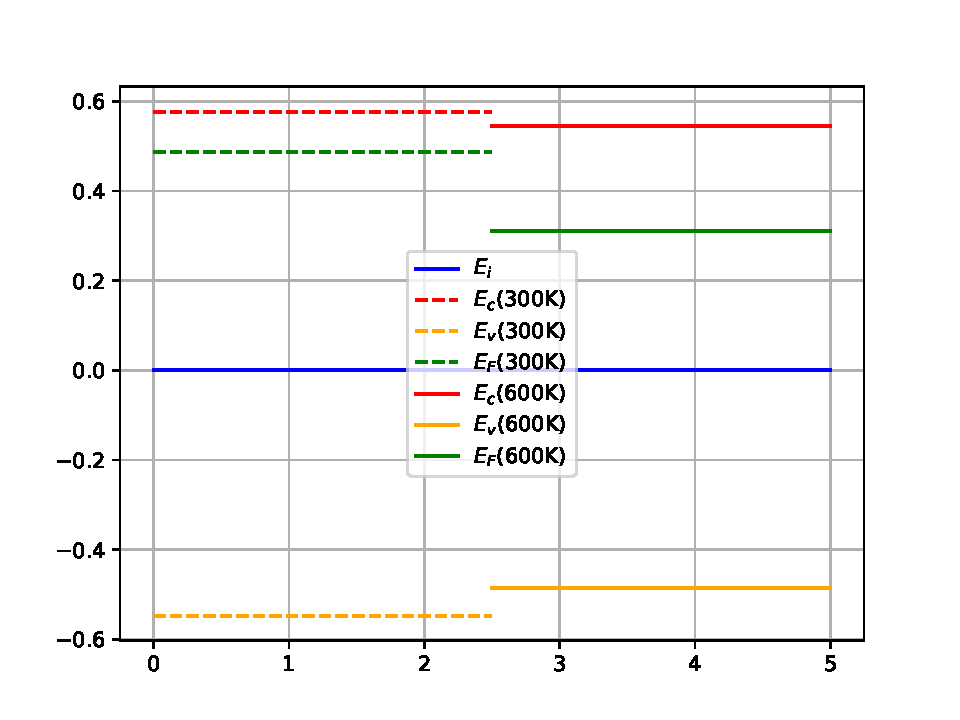
\includegraphics[width=0.9\linewidth]{Cuerpo/Ch_01/Ejercicio_01_6.pdf}
	\end{center}
\end{texercise}


\begin{texercise}
	Calcular el nivel de Fermi y dibujar el diagrama de bandas completo de silicio dopado con $10^{15}$, $10^{17}$ y $10^{19}$ átomos/cm$^3$ de P ($E_D = 0.045$ eV) a temperatura ambiente suponiendo ionización total de las impurezas. A partir del nivel de Fermi calculado comprobar si esta suposición es correcta para cada valor de dopado. Asumir que los átomos donadores ionizados vienen dados por la expresión:

	\begin{equation}
		N_D^+ = \frac{N_D}{1 + 2 \exp \left( \frac{E_F - E_D}{kT} \right)}
	\end{equation}
	\tcblower
	La solución del ejercicio pasa por calcular los valores de los niveles de Fermi usando la ecuación
	\begin{equation}
		E_F = E_i + kT \ln \parentesis{\frac{N_D}{n_i}}
	\end{equation}
	ya que estamos ante un dador que tiene todos los átomos excitados $N_D$ tal que $N_D>>n_i,N_A$. Dado que consideramos esto a tempeartura ambiente, tenemos que $n_i=$ y por tanto que para estos $N_D$:
	\begin{equation}
		N_D=10^{15} \ \cm^{-3} \Rightarrow E_F = 
	\end{equation}
	\begin{equation}
		N_D=10^{17} \ \cm^{-3} \Rightarrow E_F = 
	\end{equation}
	\begin{equation}
		N_D=10^{19} \ \cm^{-3} \Rightarrow E_F = 
	\end{equation}
	Una vez tenemos estos valores de $E_F$, veamos si es válido asumir que todosl os átomos donadores están ionizados, usando que 

	\begin{equation}
		N_D^+ = \frac{N_D}{1+2\exp\ccorchetes{(E_F-E_D)kT}}
	\end{equation}
	Tal que para las energías dadas:

	\begin{equation}
		E_F=  \Rightarrow N_D^+ = 
	\end{equation}
	\begin{equation}
		E_F = \Rightarrow N_D^+ = 
	\end{equation}
	\begin{equation}
		E_F = \Rightarrow N_D^+ = 
	\end{equation}
\end{texercise}


\begin{texercise}
	Responde a las siguientes cuestiones: 

	\begin{enumerate}
  	  \item[a)] Utilizando la expresión para los átomos donadores ionizados dada en el ejercicio anterior, calcular la concentración de donadores sin ionizar para una muestra de silicio dopada con $10^{16}$ átomos/cm$^3$ de P ($E_D = 0.045$ eV) a una temperatura de 50 K. El nivel de Fermi está situado a 0.0459 eV por debajo de la banda de conducción.
    
   	 \item[b)] Una muestra de silicio a $T = 300$ K contiene una concentración de impurezas aceptoras $N_A = 10^{16}$ cm$^{-3}$. Determinar la concentración de átomos donantes que debe ser añadida para que el silicio sea tipo N y la energía de Fermi esté 0.25 eV por debajo del borde de la banda de conducción.
	\end{enumerate}
	
	\tcblower
	Hola
\end{texercise}


\begin{texercise}
	Responde a las siguientes cuestiones: 
	\begin{enumerate}
		\item[a)] Calcular la resistividad del GaAs intrínseco a temperatura ambiente ($\mu_n = 9200$ cm$^2$/Vs, $\mu_p = 320$ cm$^2$/Vs).
		
		\item[b)] La movilidad de los electrones en el silicio es $\mu_n = 1300$ cm$^2$/Vs a temperatura ambiente. Si asumimos que la movilidad está limitada principalmente por la dispersión con la red cristalina, calcular la movilidad a $T= 150$ K.
		
		\item[c)] Dos mecanismos de dispersión tienen lugar en un semiconductor. Si sólo el primer de los mecanismos está presente la movilidad es de 250 cm$^2$/Vs. Si sólo el segundo de los mecanismos está presente la movilidad es de 650 cm$^2$/Vs. Calcular la movilidad cuando los dos mecanismos están presentes.
	\end{enumerate}
	
	\tcblower
	Hola
\end{texercise}

%%%%%%%%%%%%%%%%%%%%%%%%%%%%%%%%%%%%%%%%%%%%%%%%%%%%%%%%%%%%%%%%%%%%%%%
%%%%%%%%%%%%%%%%%%%%%%%%  SOLUCION %%%%%%%%%%%%%%%%%%%%%%%%%%%%%%%%%%%
%%%%%%%%%%%%%%%%%%%%%%%%%%%%%%%%%%%%%%%%%%%%%%%%%%%%%%%%%%%%%%%%%%%%%%%

\tcbstoprecording

\begin{Anotacion}
	\textcolor{red}{Revisar ejercicios 1,2,3,4. Hechos en la pizarra, copiados en clase. Posiblidad de error: alta.}
\end{Anotacion}

\section{Solucion}

\tcbinputrecords







\newpage

\section*{Ejercicios}
\addcontentsline{toc}{section}{\textit{Ejercicios}}

\begin{Enunciado}
\subsection*{Ejercicio 1}


	Se dopa silicio con Boro (B) en una proporción de 2 ppm (partes por millón)
	\begin{enumerate}[label=\alph*)]
		\item Calcula la concentración intrínseca del Si y obten una expresión de dicha concentración en función de la temperatura.
		\item Indica el tipo de conducción de este material y calcula la concentración de impurezas y la de electrones y huecos (n y p) a temperatura ambiente si todos los dopantes están ionizados.
		\item Calcula la posición del nivel de Fermi y dibuja el diagrama de bandas completo correspondiente.
		\item ¿Qué pasa si la concentración de impurezas igualase el valor de \( N_V \)? Representa gráficamente las bandas de energía frente a la concentración de impurezas usando todas las aproximaciones que conozcas.
	\end{enumerate}
	(DATO: Constante de red del Si \( a_0 = 5.431 \) Å).

\end{Enunciado}

	Veamos las soluciones por apartados
	\begin{enumerate}[label=\alph*)]
		\item La concentración intrínseca del Silicio en un semiconductor es el número de portadores $n_i$ en el semiconductor, si no estuviera dopado. No hay que confundir la concentración intrínseca $n_i$ con la concentración $n$, en la que si se tendrá en cuenta que el material está dopado. La concentración intrínseca es:

		      \begin{equation}
			      n_i = \sqrt{N_cN_v} e^{-E_G/2kT}
		      \end{equation}
		      donde $E_G=E_c-E-v$, y además

		      \begin{equation}
			      N_{C,V} = 2 \parentesis{\frac{m_{e,p}^* kT}{2\pi\hbar^2}}^{-3/2}
		      \end{equation}
		      Las masass $m_p^*= 1.18m_e$ y $m_n^*=0.81m_e$. Si queremos dar el valor:

		      \begin{equation}
			      N_c = 3.22 \cdot 10^{19} \cm^{-3} \tquad 	N_v = 1.83 \cdot 10^{19} \cm^{-3}
		      \end{equation}
		      De lo que se deduce

		      \begin{equation}
			      n_i = 9.56 \cdot 10^9 \cm^{-3}
		      \end{equation}


		\item Están dopando con boro, que es del grupo III, y por tanto es un dador. Esto significa que será un conductor tipo $p$. Para calcular la concentración de impurezas, primero tenemos que obtener la densidad de Boro en nuestro silicio. La densidad del silicio se calcular a partir de la constante de red y sabiendo que posee una red diamante. Así pues:
		      \begin{equation}
			      N_{Si} = \frac{8}{a_0^3}
		      \end{equation}
		      de lo que se puede deducir entonces que:
		      \begin{equation}
			      N_B = 2\cdot 10^{-6} \cdot N_{Si} = 9.988 \cdot 10^16 \cm^{-3}
		      \end{equation}
		      Nos dicen que todos los dopantes están ionizados, es decir, que estamos en el régimen extrínseco. En este régimen todos los átomos de Boro son impurezas, tal que $N_A^-=N_A=N_B$. Suponiendo que $N_A^- \gg N_D^+$, tenemos que la ecuación de neutralidad de carga:

		      \begin{equation}
			      n\cdot p = n_i^2 \tquad p-n-N_A = 0
		      \end{equation}
		      usando estas ecuaciones para despejar el valor de $n$ y $p$, tenemos que:
		      \begin{equation}
			      p = \frac{N_A}{2} + \ccorchetes{\parentesis{\frac{N_A}{2}}^2 + n_i^2}^{1/2}
		      \end{equation}
		      y luego calculamos

		      \begin{equation}
			      n = \frac{n_i^2}{p}
		      \end{equation}
		      Numéricamente podemos obtener los resultados:

		      \begin{equation}
			      n=915.034 \cm^{-3} \quad p = 9.988 \cdot 10^{16} \cm^3
		      \end{equation}


		\item La posición del nivel de Fermi de un semiconductor dopado se calcula a partir del nivel de Fermi intrínseco. Así pues
		      \begin{equation}
			      E_{Fi} = E_i = \frac{E_c+E_v}{2} + \frac{3 kT}{4} \ln \frac{m_p^*}{m_e^*} = 0.523 \text{eV}
		      \end{equation}
		      tal que la energía de Fermi. *Introducir imagen*
		      \begin{equation}
			      E_F = E_i + kT \ln \parentesis{\frac{p}{n_i}} = 0.135 \text{0.135}
		      \end{equation}
		\item Cuando la concentración de impurezas es igual al valor de $N_V$, dado que $p=N_V e^{(E_v-E_F)/kT}$, esto implicaría que $E_v = E_F$, y que por tanto la condición de \textit{semiconductor no degnerado} $E_F>E_v + 3kT$ no se cumpliría. \textit{Tenemos un semiconductor degenerado, teniendo que calcular los valores de $n$ y $p$ mediante las integrales explícitas}. Consecuentemente, estamos ante un semiconductor degenerado. *Introducir imagen para las bandas*.
	\end{enumerate}
\begin{Enunciado}
\subsection*{Ejercicio 2}

	Una muestra de Si está dopada con \( 6 \times 10^{15} \) átomos de As por cm$^3$
	\begin{enumerate}[label=\alph*)]
		\item ¿Cuál es la concentración de portadores en la muestra de Si a 300 K?
		\item ¿Cuál es la concentración de portadores a 470 K?
		\item Para cada una de las dos temperaturas anteriores determinar la posición de \( E_i \), calcular \( E_F - E_i \) y dibujar a escala el diagrama de bandas de energía para la muestra.
		\item Si dopamos el Si con \( 10^{16} \) átomos donadores y \( 5 \times 10^{15} \) átomos aceptores por cm$^3$. ¿Cuál es la concentración de portadores a 300 K?+
		\item Partimos de una muestra de Si puro y lo dopamos exclusivamente con \( 10^{14} \) átomos donadores y \( 10^{14} \) átomos aceptores por cm³. Calcula la concentración de portadores y explica el resultado obtenido.
	\end{enumerate}
	Tener en cuenta que \( E_G = 1.08 \) eV a 470 K y suponer que \( m_e^*/m_h^* = 0.69 \) es independiente de la temperatura.

\end{Enunciado}

	\begin{enumerate}[label=\alph*)]
		\item Tenemos primero que ver si está degenerado, sin embargo sabemos que para esta temperatura y el nivel de dopamiento no debería estar degenerado, y por tanto podríamos usar la ley de acción de masas junto con la condición de electroneutralidad para despejar $n$ en función de $N_D,N_A$ y $n_i$. Se puede obtener, dado que $N_D \gg n_i,N_A$, tenemos que

		      \begin{equation}
			      n\approx N_D = 6\cdot 10^{15} \cm^{-3} \tquad n\cdot p = n_i^2 \Rightarrow p = 1.67 \cdot 10^4 \cm^{-3}
		      \end{equation}
		\item Nos dicen que a $T=470$K y que $E_G=1.08$eV. Lo único que no cambio es $N_D$. Lógicamente el número de portadores intrínsecos $n_i$ cambia al aumentar la temperatura: a mayor energía térmica promocionan más electrones, mas electrones van a poder excitarse desde la banda de valencia. Calculamos $n_i$ a partir de
		      \begin{equation}
			      n_i = \sqrt{N_cN_v} e^{-E_g/2kT}
		      \end{equation}
		      Luego solo tenemos que hacer

		      \begin{equation}
			      N_{c,v} = 4.829\cdot 10^{15} T^{3/2} \parentesis{\frac{m_{n,p}^*}{m_e}}
		      \end{equation}
		      A esta temperatura tenemos entonces que:

		      \begin{equation}
			      N_c = 6.3 \cdot 10^{19} \cm^{-3} \quad N_v = 3.6 \cdot 10^{19} \cm^{-3}
		      \end{equation}
		      Y por tanto

		      \begin{equation}
			      n_i = 7.74 \cdot 10^{13} \cm^{-3}
		      \end{equation}
		      De lo que se deduce, de nuevo, aplicnado la ley de acción de masas:

		      \begin{equation}
			      n=6.001 \cdot 10^{15} \cm^{-3} \quad p = 9.98 \cdot 10^{11} \cm^{-3}
		      \end{equation}
		\item Determina la posción del nivel de Fermi intrínseco. Es secillo que:
		      \begin{equation}
			      E_i = \frac{E_c + E_v}{2} + \frac{3}{4} kT \ln \parentesis{\frac{m_p^*}{m_n^*}}
		      \end{equation}
		      Una vez tenemos $E_i$ para cada una de las temperaturas, calculamos la temperatura final
		      \begin{equation}
			      E_F = E_i + kT \ln \parentesis{\frac{n}{n_i}}
		      \end{equation}
		      *Introducir imagen*
		\item.
		\item
	\end{enumerate}
    
\begin{Anotacion}
    \textcolor{red}{\textbf{Falta por acabar}}
\end{Anotacion}
\begin{Enunciado}
\subsection*{Ejercicio 3}

	Cuestiones sobre el nivel de Fermi:

	\begin{enumerate}[label=\alph*)]
		\item Calcular la temperatura \( T \) para que el nivel de Fermi de un cristal de Silicio tipo N con \( N_D = 10^{16} \) cm\(^{-3}\) quedara a una energía \( E_G/3 \) por debajo de la banda de conducción. Suponer que \( N_C \) y \( E_G \) son constantes con la temperatura e iguales a sus valores a temperatura ambiente. Y repetir para el caso de dopar con \( N_D = 10^{18} \) cm\(^{-3}\).

		\item En un semiconductor determinado, la probabilidad de que los electrones ocupen un estado de energía \( kT \), por encima del extremo inferior de la banda de conducción es \( e^{-10} \). Determinar la posición del nivel de Fermi en dicho material.

		\item ¿Cuál es la probabilidad de que un estado de energía \( kT \) por debajo del nivel de Fermi esté ocupado por un hueco?
	\end{enumerate}

\end{Enunciado}

	\begin{enumerate}[label=\alph*)]
		\item La solución es $T=536.206$K. Para esto tenemos que usar la relación
		      \begin{equation}
			      T = \frac{E_F-E_c}{k} \frac{1}{\ln (N_D/N_c)} =  \frac{-E_g}{3k} \frac{1}{\ln (N_D/N_c)}
		      \end{equation}
		      donde $N_c=3.22\cdot 10^{19}\cm^{-3}$.
		\item Queremos calcular la posición del nivel de Fermi. Usamos la fórmula
		      \begin{equation}
			      f(E) = \frac{1}{1+e^{(E-E_F)/kT}}
		      \end{equation}
		      y usando lo que nos da el enunciado:
		      \begin{equation}
			      f(kT+E_c) = \frac{1}{1+e^{(kT+E_c-E_F)/kT}}
			      = \frac{1}{e^{10}}
		      \end{equation}
		      Tenemos entonces que

		      \begin{equation}
			      1+e^{\frac{kT+E_c-E_f}{kT}} = e^{10}
		      \end{equation}
		      De lo que se deduce que $E_F = E_c + 9kT$.
		\item ¿Cuál es la probabilidad de que un estado de energía \( kT \) por debajo del nivel de Fermi esté ocupado por un hueco? Tenemos que
		      \begin{equation}
			      1-f(E_F-kT) = 1 - \frac{1}{1+e^{-1}} \simeq 0.2689 \rightarrow 26.89 \%
		      \end{equation}
		      La probabilidad es no nula y por tanto... (preguntar a Elisa Casal).
	\end{enumerate}

\begin{Enunciado}
\subsection*{Ejercicio 4}

Responde a las siguientes cuestiones:
\begin{enumerate}
	\item[a)] A 300 K la densidad efectiva de estados en la banda de valencia es $1.83 \times 10^{19} \text{ cm}^{-3}$ para el silicio y $9.0 \times 10^{18} \text{ cm}^{-3}$ para el GaAs. Calcular sus correspondientes masas efectivas para los huecos. Comparar estas masas con la masa del electrón en el vacío.

	\item[b)] Calcula y representa la posición del nivel intrínseco en silicio a temperatura ambiente y a 1000 $^{\circ}$C (tomamos $m_p = 1.0m_0$ y $m_n = 0.19m_0$), asumiendo que el gap se mantiene constante. ¿Es razonable asumir que $E_i$ se encuentra en la mitad de la banda prohibida?
\end{enumerate}
\end{Enunciado}

\begin{enumerate}[label=\alph*)]
	\item	Tenemos que calcular la masa efectiva de los huecos para dos semiconductores diferentes, dado su densidad efectiva de estados en la banda de valencia. Esto significa que necesitamos invertir la fórmula típica, tal que
		  \begin{equation}
			  N_V = 2 \parentesis{\frac{m_p^* kT}{2\pi\hbar^2}}^{3/2} \quad \Rightarrow \quad m_p^* = \parentesis{\frac{N_V}{2}}^{2/3} {\frac{2 \pi \hbar^2}{kT}}
		  \end{equation}
		  De lo que se deduce que para el Si y el GsAs:

		  \begin{equation}
			  \text{Si:} \quad m_p^* = 7.38\cdot10^{-31} \text{kg} = 0.81 \ {m}_e
		  \end{equation}
		  \begin{equation}
			  \text{GaSi:}\quad m_p^* = 4.59 \cdot10^{-31} \text{kg} = 0.51 \ {m}_e
		  \end{equation}
		  Nivel intríseco 300K 1.7505319217070854
	\item Tenemos que calcular la posición del nivel intrínseco $E_i$ a la temperatura ambiente (300 K) y a 1000 $^\circ C$, asumiendo que $E_g$ es constante. Veamos que solo es aplicar una fórmula:
		  \begin{equation}
			  E_i = \frac{E_c+E_v}{2} + \frac{3}{4} kT \ln\parentesis{\frac{m_p^*}{m_n^*}}
		  \end{equation}
		  donde hemos considerado que $E_g=1.12$ en el silicio, y que $E_v=0$, ergo $E_c=1.12$. Hacemos la representación gráficamente. Las energías son: $300K: \ E_i=0.57$ eV y a 1273K $E_i: 0.70$ eV. Las masas usadas a 300K son: $m_p=0.81m_e$ y $m_n=1.18m_e$.
		  \begin{center}
			  \includegraphics[width=0.6\textwidth]{Ejercicios/Ch_01/Ejercicio_01_5.pdf}
		  \end{center}
		  Viendo esta imagén no parece descabellado consdierar $E_i$ constante.
\end{enumerate}


\begin{Enunciado}
	
\subsection*{Ejercicio 5}

\begin{enumerate}[label=\alph*)]
	\item En GaN a 300 K, $E_G = 3.43$ eV, $m_n^*/m_0 = 0.2$, $m_p^*/m_0 = 1.25$ y $n_i = 1.37 \times 10^{-10} \text{ cm}^{-3}$. Explicar cualitativamente (sin utilizar la fórmula que calcula el valor de $E_i$) si el nivel de Fermi intrínseco en InSb estará más próximo a la $E_C$ o a la $E_V$. Comprobarlo a continuación usando la fórmula.

	\item Las distribuciones de portadores, o número de portadores en función de la energía en las bandas de conducción y de valencia presentan un máximo a una energía próxima a los bordes de las bandas. Considerando el semiconductor como no degenerado, calcular la energía a la que se encuentra el máximo en la distribución de electrones.
\end{enumerate}
\end{Enunciado}


\begin{enumerate}[label=\alph*)]
	\item El nivel de Fermi intrínseco a temperatura no nula está mas cerca de $E_c$ si la masa efectiva de los huecos es mayor que la masa efectiva de los electrones, y más cerca de $E_v$ si la masa de los electrones es mas grande que la de los huecos. ¿Por qué? Como sabemos, la masa efectiva de los electrones/huecos es inversamente proporcional a la curvatura en el mínimo/máximo de la banda de conducción/valencia. Cuanto mayor sea la curvatura, mas energía se tiene que darse para ocupar la misma cantidad de estados. Como consecuencia, la energía de fermi intríseca, que se define como la mitad del valor entre $E_c$ y $E_v$ tendría que tirar hacia la banda con más curvatura, i.e. la que tiene menos masa efectiva. \textcolor{BrickRed}{Francamente no me tiene mucho sentido, ya que $E_c$ y $E_v$ no debería cambiar. Existen otras formas de verlo a través de la función de Fermi y la densidad de estados, habría que investigarlo.}

	En nuestro caso esto implica que \textit{debería estár mas cerca de la banda de conducción}. Para los valores dados, tenemos que

	\begin{equation}
		  E_i = \frac{E_c+E_v}{2} + \frac{3}{4} kT \ln\parentesis{\frac{m_p^*}{m_n^*}} = 1.75 \ \text{eV}
	\end{equation}
	que considerando $E_v=0$ y $E_c=E_g=3.43$ eV vemos que está mas cerca de la banda de conducción $E_c$ que de $E_v$.
	\item La concentración de electrones en la banda de conducción está dada por:

		  \[
			  n(E) = g_c(E) f(E)
		  \]

		  donde

		  \begin{itemize}
			  \item La densidad de estados en la banda de conducción es:

					\[
						g_c(E) = \frac{8\pi \sqrt{2} m_c^{3/2}}{h^3} (E - E_c)^{1/2}
					\]

			  \item La función de distribución de Fermi-Dirac en la aproximación no degenerada (Maxwell-Boltzmann) es:

					\[
						f(E) \approx e^{-\frac{(E - E_F)}{k_B T}}
					\]
		  \end{itemize}

		  Por lo que la distribución de portadores en la banda de conducción es:

		  \[
			  n(E) = \frac{8\pi \sqrt{2} m_c^{3/2}}{h^3} (E - E_c)^{1/2} e^{-\frac{(E - E_F)}{k_B T}}
		  \]

		  Para encontrar el máximo, derivamos respecto a \( E \) e igualamos a cero:

		  \[
			  \frac{d}{dE} \left[ (E - E_c)^{1/2} e^{-\frac{(E - E_F)}{k_B T}} \right] = 0
		  \]

		  Aplicando la regla del producto:

		  \[
			  \frac{1}{2} (E - E_c)^{-1/2} e^{-\frac{(E - E_F)}{k_B T}} + (E - E_c)^{1/2} e^{-\frac{(E - E_F)}{k_B T}} \left(-\frac{1}{k_B T} \right) = 0
		  \]

		  Factorizando:

		  \[
			  e^{-\frac{(E - E_F)}{k_B T}} (E - E_c)^{-1/2} \left[ \frac{1}{2} - \frac{(E - E_c)}{k_B T} \right] = 0
		  \]

		  Para que se cumpla la igualdad, la expresión entre corchetes debe ser cero:

		  \[
			  \frac{1}{2} = \frac{(E - E_c)}{k_B T}
		  \]

		  Despejando \( E \):

		  \[
			  E - E_c = \frac{1}{2} k_B T
		  \]
		  Por lo tanto, el máximo de la distribución de electrones en la banda de conducción se encuentra a:

		  \[
			  E_{\text{max}, c} = E_c + \frac{1}{2} k_B T
		  \]

		  Siguiendo el mismo procedimiento para los huecos en la banda de valencia:

		  \[
			  E_{\text{max}, v} = E_v - \frac{1}{2} k_B T
		  \]

		  Esto significa que los portadores tienden a concentrarse en energías lige,amente por encima del borde de la banda de conducción y por debajo del borde de la banda de valencia en aproximadamente \( \frac{1}{2} k_B T \). El doctorando hizo un dibujo que dijo que sale en el Pierret, sobre la multiplicación de producto de la densidad de estados y las bandas. Véase notas a mano.

\end{enumerate}


\begin{Enunciado}
\subsection*{Ejercicio 6}

Dibujar un diagrama de bandas para el silicio dopado con $10^{17}$ átomos/cm$^3$ de arsénico a 300 K y 600 K. Mostrar el nivel de Fermi, $E_C$, $E_V$ y utilizar el nivel de Fermi intrínseco como energía de referencia, asumiendo el caso de ionización total. La variación del bandgap con la temperatura viene dada por la expresión de Varshni (DOI: 10.1016/0031-8914(67)90062-6):

\begin{equation}
	E_G(T) = E_G(0) - \frac{\alpha T^2}{T + \beta}
\end{equation}

Para el silicio $\alpha = 4.73 \times 10^{-4} \text{ eV/K}$, $\beta = 636 \text{ K}$ y $E_G(0) = 1.17 \text{ eV}$. Suponer que las masas efectivas se mantienen constantes con la temperatura.

\end{Enunciado}


Nos dicen que dibujemos un diagrama de bandas para el silicio dopado por arsénico (grupo V, dador) completamente ionizado. Esto implica necesariamente calcular $E_i,E_c,E_v$ y $E_F$. Primero vamos a despejar $E_i$ y $E_v$, luego despejaremos en función de estos $E_F$. Recordar que

\begin{equation}
	E_i = \frac{E_v+E_c}{2} - \frac{3}{4} kT \ln\parentesis{\frac{m_n^*}{m_p^*}}
\end{equation}

\begin{itemize}
	\item Como hemos dicho despejamos estas energías. Dado que $E_i$ es nuestra referencia, las ecuaciones a usar son, a una $T$ dada, que:
		  \begin{equation}
			  E_c-E_v = E_g(0) - \frac{\alpha T^2}{T+\beta} \qquad E_c+E_v=-2 \cdot \frac{3}{4} kT\ln \parentesis{\frac{m_n^*}{m_p^*}}
		  \end{equation}
		  De lo cual se deduce que:
		  \begin{equation}
			  E_c = \frac{1}{2} \ccorchetes{E_g(0) - \frac{\alpha T^2}{T+\beta} - \frac{3}{2} kT^{3/2} \ln \parentesis{\frac{m_n^*}{m_p^*}}}
		  \end{equation}
		  \begin{equation}
			  E_v = \frac{1}{2} \ccorchetes{-E_g(0) +\frac{\alpha T^2}{T+\beta} - \frac{3}{2} kT^{3/2} \ln \parentesis{\frac{m_n^*}{m_p^*}}}
		  \end{equation}
		  Usando las masas de portadores $m_n^*=1.18m_e$ y $m_p^*=0.81m_e$  (y considerado, como nos dice el enunciado, que son constantes frente a la tempratura). Obteniendo los siguientes resultados numéricos:
		  \begin{equation}
			  \text{300K}: \qquad
			  E_c = 0.570 \ \text{eV} \quad E_v = -0.554 \ \text{eV}
		  \end{equation}
		  \begin{equation}
			  \text{600K}: \qquad
			  E_c = 0.531  \ \text{eV} \quad E_v = -0.502\ \text{eV}
		  \end{equation}
	\item Ahora tenemos que calcular $E_F$, que viene dado, en un conductor dopado $N$ no degnerado por (recordar que $E_i=0$)
		  \begin{equation}
			  E_F = kT \ln \parentesis{\frac{N_D}{n_i}}
		  \end{equation}
		  Dado que conocemos $T$ y $N_D$, solo resta saber el valor de $n_i$, para lo cual hemos usado la expresión:

		  \begin{equation}
			  n_i = \sqrt{N_c N_v} e^{-E_g/2kT}
		  \end{equation}
		  siendo $N_c$ y $N_v$ las típicas funciones que dependen de la masa efectiva y del a temperatura. Así pues, obtenemo los resultados:
		  \begin{equation}
			  \text{300K:}\quad
			  E_F = 0.420 \ \text{eV} \qquad
			  \text{600K:}\quad
			  E_F= 0.178 \ \text{eV}
		  \end{equation}
\end{itemize}
Una vez tenemos esto podemos realizar la representación:
\begin{center}
	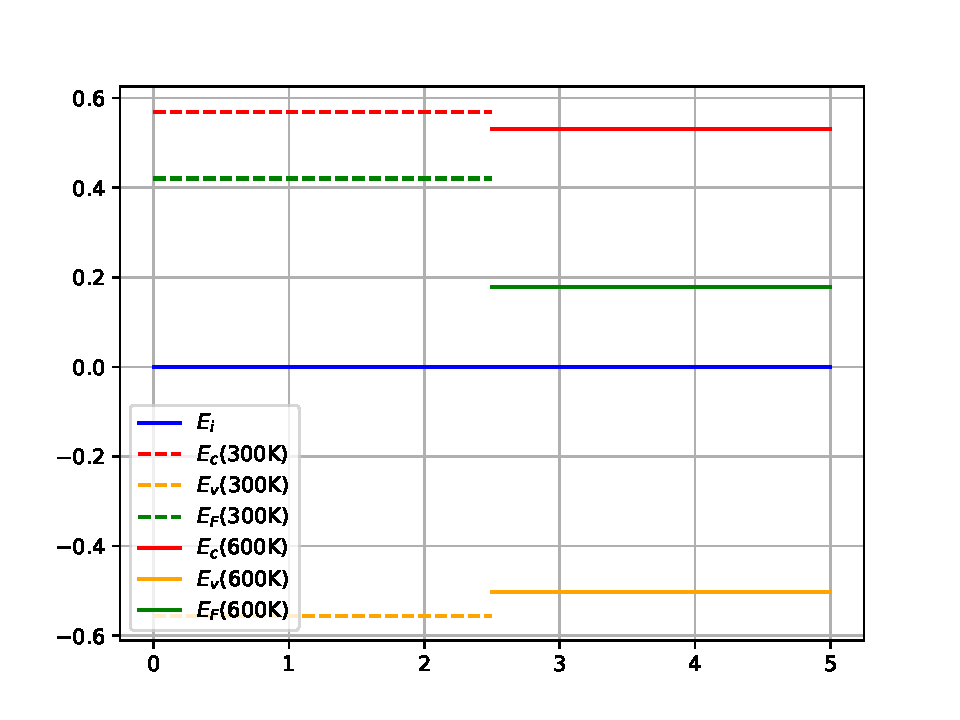
\includegraphics[width=0.9\linewidth]{Ejercicios/Ch_01/Ejercicio_01_7.pdf}
\end{center}


\begin{Enunciado}
\subsection*{Ejercicio 7}
Calcular el nivel de Fermi y dibujar el diagrama de bandas completo de silicio dopado con $10^{15}$, $10^{17}$ y $10^{19}$ átomos/cm$^3$ de P ($E_D = 0.045$ eV) a temperatura ambiente suponiendo ionización total de las impurezas. A partir del nivel de Fermi calculado comprobar si esta suposición es correcta para cada valor de dopado. Asumir que los átomos donadores ionizados vienen dados por la expresión:

\begin{equation}
	N_D^+ = \frac{N_D}{1 + 2 \exp \left( \frac{E_F - E_D}{kT} \right)}
\end{equation}
\end{Enunciado}

La solución del ejercicio pasa por calcular los valores de los niveles de Fermi usando la ecuación
\begin{equation}
	E_F = E_i + kT \ln \parentesis{\frac{N_D}{n_i}}
\end{equation}
Recordemos que en este caso definimos $E_{c}=0$ eV. Consecuentemente tanto $E_D$ como $E_F$ serán negativos. Estamos ante un dador que tiene todos los átomos excitados $N_D$ tal que $N_D>>n_i,N_A$. Dado que consideramos esto a tempeartura ambiente, tenemos que $n_i=1.18\cdot 10^{10} \ \cm^{-3}$ y por tanto que para estos $N_D$:
\begin{equation}
	N_D=10^{15} \ \cm^{-3} \Rightarrow E_F = -0.27 \ \eV
\end{equation}
\begin{equation}
	N_D=10^{17} \ \cm^{-3} \Rightarrow E_F = -0.15  \ \eV
\end{equation}
\begin{equation}
	N_D=10^{19} \ \cm^{-3} \Rightarrow E_F = -0.035  \eV
\end{equation}
Una vez tenemos estos valores de $E_F$, veamos si es válido asumir que todosl os átomos donadores están ionizados, usando que

\begin{equation}
	N_D^+ = \frac{N_D}{1+2\exp\ccorchetes{(E_F-E_D)kT}}
\end{equation}
Tal que para las energías dadas:
\begin{equation}
	E_F= -0.27  \ \eV \Rightarrow N_D^+ =  9.999\cdot 10^{14}  \ \cm^{-3}
\end{equation}
\begin{equation}
	E_F = -0.15 \ \eV\Rightarrow N_D^+ =  9.722\cdot 10^{16} \ \cm^{-3}
\end{equation}
\begin{equation}
	E_F =-0.034 \ \eV \Rightarrow N_D^+ = 2.597 \cdot 10^{18}  \ \cm^{-3}
\end{equation}
Dibujamos los gráficos
\begin{center}
	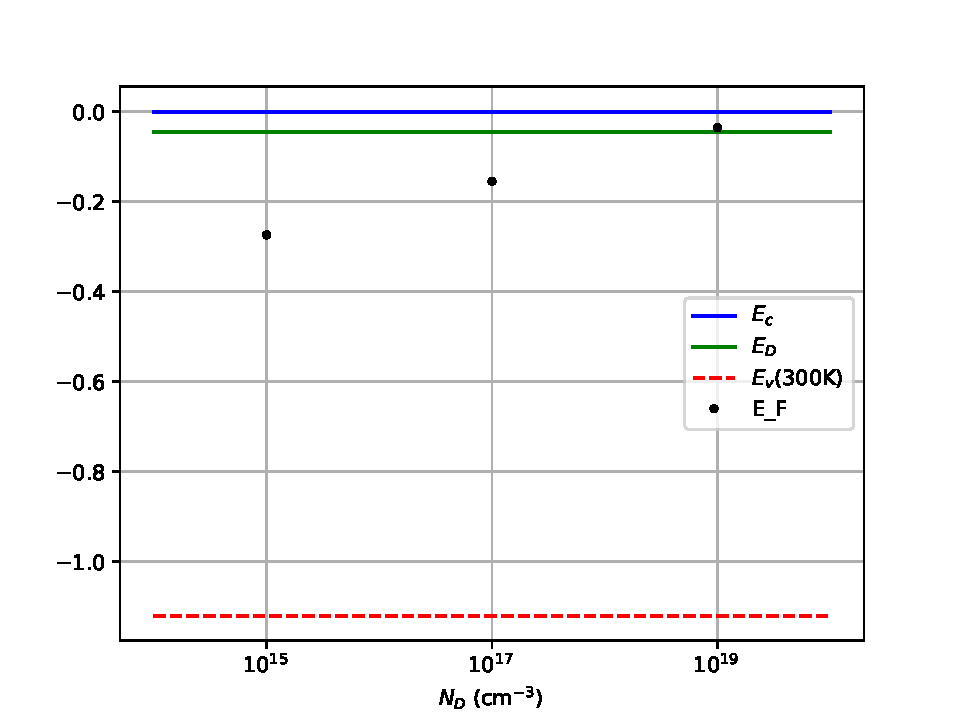
\includegraphics[width=0.9\linewidth]{Ejercicios/Ch_01/Ejercicio_01_8.pdf}
\end{center}



\begin{Enunciado}
\subsection*{Ejercicio 8}

Responde a las siguientes cuestiones:

\begin{enumerate}
	\item[a)] Utilizando la expresión para los átomos donadores ionizados dada en el ejercicio anterior, calcular la concentración de donadores sin ionizar para una muestra de silicio dopada con $10^{16}$ átomos/cm$^3$ de P ($E_D = 0.045$ eV) a una temperatura de 50 K. El nivel de Fermi está situado a 0.0459 eV por debajo de la banda de conducción.

	\item[b)] Una muestra de silicio a $T = 300$ K contiene una concentración de impurezas aceptoras $N_A = 10^{16}$ cm$^{-3}$. Determinar la concentración de átomos donantes que debe ser añadida para que el silicio sea tipo N y la energía de Fermi esté 0.25 eV por debajo del borde de la banda de conducción.
\end{enumerate}
\end{Enunciado}

\lipsum[1]




\chapter{Simetrías}

Las simetrías en la física están asociadas a las leyes deconservación, y sus implicaciones en la dinámica quedaron completamente entendidas en 1918 con la publicación del \textit{teorema de Noether} en 1918. Este teorema establece qeu cada simetría nos lleva a una ley de conservación y viceversa: cada ley de conservación debe tener su simetría. 

En particular tenemos varias simerias y vairas leyes de cosnervación asociadas a los procesos físicos. Por ejemplo, cuando un fenómeno se puede trasladar en el tiempo conserva la energía, cuando lo hacemos en el espacio conserva momento, cuando lo podemos rotar conserva momento angular, y cuando le podemos aplicar trasformaciones Gauge conserva carga (bien carga eléctrica, carga de isospín débil o color). 

\section{Momento angular y espín}

El \textbf{espín} es una propiedad intrínseca de las partículas, y se comporta como un momento angular. Para cada tipo de particula elemental está fijada, mientras que los estados compuestos (por ejemplo, dos electrones interaccionando) pueden presentar espines diferentes. 

\subsection{Estados de partículas espin 1/2}

Las partículas con espín 1/2 se pueden representar en \textbf{espinores}, que es un vector columna de 2 columnas. Se representa como $|S,S_3 \rangle $ donde $S=1/2$ y $S_3=\pm 1/2$, con dos estados posibles. 

\begin{equation}
    |1/2,1/2 \rangle  = \begin{pmatrix}
         1 \\ 0 
    \end{pmatrix} \qquad
    |1/2,-1/2 \rangle  = \begin{pmatrix}
        0 \\ 1 
    \end{pmatrix}
\end{equation}
El estado más general posible sería: 

\begin{equation}
    \psi = \alpha 
    |1/2,1/2 \rangle  + \beta 
    |1/2,-1/2 \rangle   = \begin{pmatrix}
        \alpha \\ 
        \beta
    \end{pmatrix}
\end{equation}
donde $\alpha^2 + \beta^2 = 1$. 

\section{Isospín}

Tras el descubrimiento del neutrón en 1932 Heisenberg observó qeu el neutrón era prácticamente igual al proton (a parte de la carga eléctrica). En este contexto Heisenberg propuso que el protón y neutron en realidad eran la misma partícula  (el nucleón) pero en dos estados diferentes:

\begin{align}
    N &= \begin{pmatrix} \alpha \\ \beta \end{pmatrix} \nonumber \\
    p &= \begin{pmatrix} 1 \\ 0 \end{pmatrix} \nonumber \\
    n &= \begin{pmatrix} 0 \\ 1 \end{pmatrix}
\end{align}

Como podemos ver, la forma, el álgebra, es análoga completamente a la representación de las partículas con espín 1/2. Hablamos entonces de \textbf{isospín} $\In$ con componentes $I_1,I_2$ e $I_3$ como conceptos abstractos similares al momento angular. El isospín es adimensional por convención.

Las interacciones fuertes son invariantes bajo rotaciones en el espacio de isospín, al igual que las fuerzas eléctricas son inviariantes a rotaciones en una configuración espacial. Esta nueva invariancia, no relacionada con el espacio o tiempo, se le llama \textbf{simetría interna} y está relacionada con las relaciones del as partículas entre sí. 

Como sabemos por la teoría de Noether esta conservación del isospín nos lleva a a un grupo de simetría, que será el grupo SU(2). Conclusión: las interacciones fuertes son invariantes bajo rotaciones internas del grupo de simetría SU(2).

De esta forma también podremos generar estados con diferente isospín, como por ejemplo los piones $\pi$, con isospín 1, con 3 estados posibles: 

\begin{equation}
    \pi^+ = |1,+1\rangle 
    \quad \pi^0 = |1,0\rangle
    \quad \pi^- = |1,-1\rangle
\end{equation}
o el $\Lambda$ con $I=0$ y un solo estado:

\begin{equation}
    \Lambda = |0,0\rangle
\end{equation}
e incluso el $\Delta$ con $I=3/2$ y 5 estados posibles: 

\begin{equation}
    \Delta^{++} = |3/2,3/2\rangle
    \quad \Delta^+ = |3/2,1/2\rangle
    \quad \Delta^0 = |3/2,-1/2\rangle
    \quad \Delta^- = |3/2,-3/2\rangle
    \quad \Delta^{--} = |3/2,-3/2\rangle
\end{equation}
Para determinar el número de isospín $I$ de un multiplete podemos contar el número de partículas $N$ que contiene, mientras que la multiplicaidad $2I+1$ nos da el número de estados poisbles para dicha partícula. 

La tercera componente del isospín nos habla de la carga eléctrica de la partícula, por lo que es bien conocido. En el modelo de Quarks, son los quarks $u$ y $d$ los que forman dobletes de isospines, mientras que otros quarks no tienen isospín. 

\subsection{Implicaciones dinámicas del isospín}

\subsection{El problema de los 8 bariones}

\section{Paridad}

El pensamiento físico general a principio del siglo pasado era que la naturaleza era ambidiestra, es decir, que una imagen espejo de cualquier fenómeno físico representa un fenómeno físico posible e indéntico (lo describen las mismas ecuaciones). El operador es $\Pcal$, tal qeu 

\begin{equation*}
    \Pcal \psi(\rn,\pn) = \psi(-\rn,-\pn)
\end{equation*}

En 1956 T.D. Lee y C.N. Young propusieron a diferentes físicos que hicieran experimentos esta simetría era cierta, o si por el contrario había fenómenos físicos que violaran paridad. En el electromagnétismo esta simetría se cumplía, aunque no se sabía para la interacción débil.

La conclusión no se hizo esperar, y en 1957 Chien-Shiung Wu realizó un experimento con átomos de cobalto-60 y observó que la desintegración beta de los núcleos no era simétrica bajo la transformación de paridad. Este experimento fue el primero en demostrar que la interacción débil no es invariante bajo la transformación de paridad. 

\subsection{Helicidad}

La \textbf{helicidad} de una partícula es el valor de $m_s/s$ sobre el eje de propagación de la partícula, tal que:

\begin{equation}
    h = \frac{\sn \cdot \pn}{s \cdot  p}
\end{equation}
con dos posibles helicidades (en el caso de partículas con espín 1/2: +1 y -1). En el experimento de Wu solo fueron observados partículas con helicidad a izquierdas. Es claro que hacer una transformación de paridad $\rn,\pn \to -\rn,-\pn$ cambia $h$. Es decir, $h$ es sensible a la paridad. Entonces si un fenómeno viola paridad debemos ver partículas con una paridad que con otra. En el experimento de Wu se observó precisamente esto, obteniendo partícuals qeu violan paridad (fermiones) a izquierdas.

\section{Conjugación de carga}

La \textbf{conjugación de carga} $\mathcal{C}$ convierte a cada partícula en su antipartícula. Lógicamente solo puede entenderse en el contexto de la ecuación de Dirac. Este operador cambia el signo de todos los números cuánticos de carga eléctrica, número bariónico, leptónico, extrañeza... conservando masa, energía, momento y espín. 

La mayor parte de las partículas no son autoestados de $\mathcal{C}$, ya que no hay muchas partícuals que son sus propias antipartículas: fotón, $\pi^0$... Es un número cuántico multiplicativo y es conervado en el electromagnetismo  y interacciones fuertes, pero es violado en las interacciones débiles. 

\subsection{Paridad G}

Los piones cargados son autoestados del operador $\Gcal$, que se define como

\begin{equation*}
    \Gcal = \mathcal{C} \cdot \mathbb{R}_2 \qquad \mathbb{R}_2 = e^{i \pi I_2}
\end{equation*}
Todos los mesones que no porten un quark strange, charm, bottom o top son autoestados de $\Gcal$. 


\section{Violación CP}

Las interacciones débiles no son invairantes bajo paridad ni bajo conjugación de carga. Evidencias de la no conservación de paridad ya hemos explicado como fue descubierta/demostarada, mientras que la evidencia de $\Ccal$ también se puede ver que es que el decaimient $\pi^+ \to \mu^+ + \nu_\mu$ ocurre para un neutrino a izquierdas mientras que la conjugación de dicha reacción $\pi^- \to \mu^- + \bar{\nu}_\mu$ ocurre para un neutrino a derechas (y hemos dihco que espín y momento se conservavan).

Sin embargo si hacemos los cambios simultáneamente, es decir, aplicamos $\Ccal \Pcal$ sobre la reacción, vemos que es la misma reacción. La violación de CP fue demostrado a través de los kaones neutros, en 1964. Esta violación de CP podría explicar la diferencia entre materia y antemateria que parece haber en el universo. 

Para estudair esto nos fijamos en el caso de los kaones. El kaon es un mesón con extrañeza, y se puede transofmrar en un antikaon en un proceso a segundo orden en la interacción débil (hay un loop).

En el laboraotrio lo qeu se observa son combinaciones lineales de los estados $K^0$ y $\overline{K}^0$. Dado que $K^0$ es un bosón tienen la misma paridad y resulta ser psoudoescalar:

\begin{equation}
    P |K^0\rangle = - |K^0 \rangle  \qquad 
    P |\bar{K}^0\rangle = - |\bar{K}^0 \rangle 
\end{equation}
Por otro lado 

\begin{equation}
    C |K^0\rangle = - |\bar{K}^0 \rangle  \qquad 
    C |\bar{K}^0\rangle = - |{K}^0 \rangle 
\end{equation}
Luego 
\begin{equation}
    CP |K^0\rangle =  - |\bar{K}^0 \rangle  \qquad 
    CP |\bar{K}^0\rangle = - |{K}^0 \rangle 
\end{equation}
Sin embargo los auetoestados normalizados:


\begin{equation}
   |K^1\rangle = \frac{1}{\sqrt{2}} (|\bar{K}^0 \rangle - |{K}^0 \rangle )  \qquad 
   |K^2\rangle = \frac{1}{\sqrt{2}} (|\bar{K}^0 \rangle + |{K}^0 \rangle ) 
\end{equation}
tal que 
\begin{equation}
   CP|K^1\rangle = |K^1\rangle  \qquad 
   CP|K^2\rangle = - |K^2\rangle
\end{equation}
Si asumimos que CP es conservada en las interacciones débiles, $K_1$ solo puede decaer en estados con CP +1 y $K_2$ solo en estados con CP -1. Experimentalmente se distinguien, cayendo mucho más rápido $K_1$ que $K_2$. Si la invarianza CP existe los $K_2$ solo se peuden desintegrar en 3 piones, si observamos veremos que no siempre el $K_1$ cae a 2 piones y el $K_2$ a 3 piones. Consecuentemente se viola CP. 


\section{Simetría temporal y TPC}

El teoerma TCP o CPT está basado en una de los principios rectores de QFT, y nos dice que aplicar conjugación de carga, paridad y orden temporal no cambia el fenómeno físico. Sería imposible construir una teoría cuántica de campos qeu violara TCP. 
\newpage

\section*{Ejercicios}
\addcontentsline{toc}{section}{\textit{Ejercicios}}
\begin{Enunciado}
\subsection*{Ejercicio 1}

Cuestiones sobre la resistividad y movilidad:
\begin{enumerate}[label=\alph*)]
	\item La resistividad de un material tipo N es por lo regular más pequeña que la resistividad de un material tipo P de dopado comparable, explica por qué suele ocurrir esto. Calcula la resistividad del Si si se dopa con fósforo con una concentración de \( 10^{17} \) cm\(^{-3}\). Repite el cálculo para el caso en que dopemos con aluminio con la misma concentración y calcular la corriente de arrastre en ambos casos considerando un campo eléctrico de \( 10^5 \) V/cm.

	\item Calcula la densidad de impurezas necesarias para tener un cristal de Si tipo P con resistividad 0.1 \(\Omega\cdot\)cm. ¿Qué proporción hay de átomos de impureza sobre el número de átomos de Si?
		  (DATO: Constante de red del Si \( a_0 = 5.431 \) Å). Si suponemos que el semiconductor es no degenerado, ¿cuánto vale \( D_p \)?
\end{enumerate}

\end{Enunciado}




\begin{enumerate}[label=\alph*)]
	\item La diferentencia radica en la masa efectiva, que se expresa en la movilidad:
		  \begin{equation}
			  \rho = \frac{1}{q(n\mu_n + p \mu_)}
		  \end{equation}
		  Cuando $\mu_n>\mu_p \Rightarrow \rho_n < \rho_p$. Y esto siempre ocurre. Las movilidades dependen de la temperatura y la cantidad que esté dopado, por lo que puede ser diferente. Para un semiconductor dopado tipo $N$:

		  \begin{equation}
			  \rho_N = \frac{1}{qn{\mu_n}} = \frac{1}{1.6\cdot 10^{19} \cdot 10^{17}\cdot 1350}= 0.0463 \Omega \cm
		  \end{equation}
		  Y para un tipo $P$:
		  \begin{equation}
			  \rho_N = \frac{1}{1.6\cdot 10^{19} \cdot 10^{17}\cdot 480} = 0.13 \Omega \cm
		  \end{equation}
		  (valores de movilidad sacados de la Wikipedia). Ahora podemos calucular la corriente de arrastre (usamos que $J=qnN\epsilon$, donde $\epsilon = 10^5$ eV)
		  \begin{equation}
			  J_N =  2.16 \cdot 10^6  A\cm^{-2}  \tquad J_p = 7.68 \cdot 10^3  A\cm^{-2}
		  \end{equation}
	\item Ahora lo que hacemos es considerar que el número de impurezas es igual al número de huecos (están todas completamente ionizadas). Lo que nos queda entonces es:
		  \begin{equation}
			  N_A = \frac{1}{q\rho \mu_p } = \frac{1}{1.6\cdot 10^{19} \cdot 0.1 \cdot 480} = 1.3 \cdot 10^{17} \cm^{-3}
		  \end{equation}
		  Podemos calcular con $a_0$ el númerode átomos de silicio por unidad de volumen:

		  \begin{equation}
			  N_{Si} = 5 \cdot 10^{22} \text{at} \cm^{-3}
		  \end{equation}
		  Y solo tenemos, para calcular la proporción:

		  \begin{equation}
			  \frac{N_A}{N_{Si}} = 2.6 \cdot 10^{-6} = 2.6 \ \text{ppm}
		  \end{equation}
		  Para acabar necesitamos calcular la relación de Eistein (solo usable en semicdonductores no degenerados). Así tenemos que

		  \begin{equation}
			  D_p = \frac{kT}{q} \mu_p = 12.4 \cm^2 / s
		  \end{equation}
\end{enumerate}

\begin{Enunciado}
\subsection*{Ejercicio 2}

Responde a las siguientes cuestiones:
\begin{enumerate}
	\item[a)] Calcular la resistividad del GaAs intrínseco a temperatura ambiente ($\mu_n = 9200$ cm$^2$/Vs, $\mu_p = 320$ cm$^2$/Vs).

	\item[b)] La movilidad de los electrones en el silicio es $\mu_n = 1300$ cm$^2$/Vs a temperatura ambiente. Si asumimos que la movilidad está limitada principalmente por la dispersión con la red cristalina, calcular la movilidad a $T= 150$ K.

	\item[c)] Dos mecanismos de dispersión tienen lugar en un semiconductor. Si sólo el primer de los mecanismos está presente la movilidad es de 250 cm$^2$/Vs. Si sólo el segundo de los mecanismos está presente la movilidad es de 650 cm$^2$/Vs. Calcular la movilidad cuando los dos mecanismos están presentes.
\end{enumerate}

\end{Enunciado}



\begin{enumerate}[label=\alph*)]
	\item Para calcular la resistividad usamos la fórmula:
	\begin{equation}
		\rho = \frac{1}{q(\mu_p p + \mu_n n )}
	\end{equation}
	Donde solo tenemos que sustituir $n,p\rightarrow n_i$. Calculamos usando que $n_i= 2.25\times 10^6 \cm^{-3}$ de lo que se deduce que:
	\begin{equation}
	\rho =4.33\cdot 10^9 \ \Omega \cm
	\end{equation}
	\textcolor{Blue}{Creo que hay algo mal en el resultado numérico aunque la ecuación está bien. Podría dar entorno a 2.5 por diez a la diez, más o menos.}
	\item No conocemos la fórmula explícita, pero śi que sabemos que $\mu_{\text{impurezas}}\propto T^{-3/2}$ (red cristalina es igual a dispersión por fonones). Por tanto podemos calcular:
	\begin{equation}
		\frac{\mu_{\text{imp}} (T=150K)}{\mu_{\text{imp}}(T=300K)} = \parentesis{\frac{150}{300}}^{-3/2}		
	\end{equation}
	De lo que obtenemos:
	\begin{equation}
		\mu_{\text{imp}} (T=150K) = 3677 \ \cm^2 / \text{Vs}
	\end{equation}
	\item Tenemos que usar la \textit{regla mathiessen}:
	\begin{equation}
		\frac{1}{\mu} = \frac{1}{\mu_{1}}+\frac{1}{\mu_{2}} 
	\end{equation}
	De lo que obtenemos:		
	\begin{equation}
		\mu = 180.55 \ \cm^2 / \text{Vs} 
	\end{equation}
\end{enumerate}

\begin{Enunciado}
\subsection*{Ejercicio 3}
Obtener las concentraciones de electrones y huecos, movilidades y resistividades de muestras de silicio a \(300 K\) para las siguientes concentraciones de impurezas:
\begin{itemize}
	\item[(a)] \(1 \times 10^{15}\) átomos/cm$^3$ de boro.
	\item[(b)] \(1 \times 10^{16}\) átomos/cm$^3$ de boro y \(1.5 \times 10^{16}\) átomos/cm$^3$ de arsénico.
	\item[(c)] \(5 \times 10^{15}\) átomos/cm$^3$ de boro, \(10^{17}\) átomos/cm$^3$ de arsénico y \(10^{17}\) átomos/cm$^3$ de galio.
\end{itemize}
Considerar que, las movilidades para portadores mayoritarios:
\begin{equation}
	\mu_n (N) = 65  + \frac{1265}{1+\parentesis{\frac{N}{8.5\times 10^{16}}}^{0.72}} \qquad 
	\mu_p (N) = 48  + \frac{447}{1+\parentesis{\frac{N}{6.3\times 10^{16}}}^{0.76}}
\end{equation}
Para portadores minoritarios:
\begin{equation}
	\mu_n (N) = 232  + \frac{1180}{1+\parentesis{\frac{N}{8\times 10^{16}}}^{0.9}} \qquad 
	\mu_p (N) = 130  + \frac{370}{1+\parentesis{\frac{N}{8\times 10^{17}}}^{1.25}}
\end{equation}

\end{Enunciado}




Primero tenemos que evaluar si son dadores/aceptores, calcular $n$ y $p$, luego evaluar las fórmulas para portadores mayoritarios y minoritarios, y finalmente la resistividad. \textcolor{red}{Tengo que cambiar los datos, ya que $N=N_A+N_D$, teniendo que calcular n y p de una manera difernte a $p=N_D$.}  Para calcular $n$ y $p$:
\begin{enumerate}[label=\alph*)]
	\item El Boro es un átomo aceptor, por lo que tendremos como dato $N_A=10^{15} \ $átomos/$\cm^3$. Ahora calculamos, usando que $n_i=1.18\times 10^{10}$:   
	\begin{equation}
		p = N_A = 10^{15} \qquad n = \frac{n_i^2}{p} =1.39 \cdot 10^5 \cm^-3
	\end{equation}
	Calculamos las movilidades, usando la mayoritaria para los huecos y la minoritaria para los electrones:
	\begin{equation}
		\mu_p=4.77\cdot 10^2  \ \cm^2 /  \text{V s} \qquad 
		\mu_n=1.39 \cdot 10^3 \ \cm^2 /  \text{V s}
	\end{equation}
	La resistividad $\rho$ se calcula ahora fácilmente:
	\begin{equation}
		\rho = \frac{1}{e(\mu_n n + \mu_pp)} \rightarrow 
		\rho = 13.1 \ \Omega \cm
	\end{equation}

	\item El Arsénico es un átomo dador, por lo que tendremos como dato $N_{D\text{eff}}=5 \times 10^{15} \ $átomos/$\cm^3$, que se deduce de:
	\begin{equation}
		N_{D\text{eff}} = N_{\text{As}} - N_{\text{B}} = 5 \times 10^{15}
	\end{equation}
	Ahora calculamos, usando que $n_i=1.18\times 10^{10}$:   
	\begin{equation}
		n = N_{D\text{eff}} = 10^{15} \qquad p = \frac{n_i^2}{n} = 2.78 \cdot 10^4 \cm^-3
	\end{equation}
	Calculamos las movilidades, usando la mayoritaria para los electrones y la minoritaria para los huecos:
	\begin{equation}
		\mu_n=9.60 \cdot 10^2  \ \cm^2 /  \text{V s} \qquad 
		\mu_p=4.89 \cdot 10^2  \ \cm^2 /  \text{V s}
	\end{equation}
	La resistividad $\rho$ se calcula ahora fácilmente:
	\begin{equation}
		\rho = \frac{1}{e(\mu_n n + \mu_pp)} \rightarrow \rho = 1.3 \ \Omega \cm
	\end{equation}
	ESTA TODO MAL.
	\item El Galio es un átomo aceptor, por lo que tendremos como dato $N_{A\text{eff}}=5 \times 10^{15} \ $átomos/$\cm^3$, que se deduce de:
	\begin{equation}
		N_{A\text{eff}} = N_{\text{Ga}} + N_{\text{B}} - N_{\text{As}} =  2.78 \cdot 10^4 \ \cm^{-3}
	\end{equation}
	Ahora calculamos, usando que $n_i=1.18\times 10^{10}$:   
	\begin{equation}
		p = N_{A\text{eff}} = 5 \times 10^{15} \qquad p = \frac{n_i^2}{n} = 3e+04 \cm^-3
	\end{equation}
	Calculamos las movilidades, usando la mayoritaria para los huecos y la minoritaria para los electrones:
	\begin{equation}
		\mu_p=4.38 \cdot 10^{2}  \ \cm^2 /  \text{V s} \qquad 
		\mu_n=1.18 \cdot 10^{3} \ \cm^2 /  \text{V s}
	\end{equation}
	La resistividad $\rho$ se calcula ahora fácilmente:
	\begin{equation}
		\rho = \frac{1}{e(\mu_n n + \mu_pp)} \rightarrow 
		\rho = 2.85 \ \Omega \cm
	\end{equation}
	ESTA TODO MAL.
\end{enumerate}

\begin{Enunciado}
\subsection*{Ejercicio 4}

\begin{itemize}
\item[(a)] Una muestra de silicio intrínseco es dopada desde un lateral con donadores de tal forma que:
\[
	N_D = N_0 \exp(-ax).
\]
Suponiendo condiciones de equilibrio y que \(N_D \gg n_i\), encontrar la expresión del campo eléctrico interno \(E(x)\). Evaluar \(E(x)\) para \(a = 10^{-6} \, \text{m}^{-1}\).
\item[(b)] Si ahora el perfil de dopado es:
\[
	N_D(x) = N_0+(N_L-N_0)(x/L),
\]
obtener una expresión para el campo eléctrico en un plano \(x\) dentro del dispositivo, considerando constantes el coeficiente de difusión y la movilidad. ¿Cuál es la expresión de la diferencia de potencial entre las superficies frontal y trasera de la muestra si la muestra es de longitud \(L\)? Consideraremos condiciones de equilibrio térmico y eléctrico.
\end{itemize}
\end{Enunciado}


\begin{enumerate}[label=\alph*)]
	\item Nos dicen que $N_D=N_0 \exp(-ax)$, y queremos calcular $E(x)$. Dependerá del nivel de profundidad que quieres darle al ejercicio. Suponemos, al no dar datos de los procesos recombinación-generación, que estamos en el \textit{modelo de arrastre-difusión}. Así pues, tenemos que:
	\begin{equation}
		\parciales{n}{t} = \div \Jn = 0 \rightarrow \div (\Jn_{\arr}+\Jn_{\diff}) = 0 \rightarrow J_{\arr}+J_{\diff} = 0
	\end{equation}
	tal que (pasamos de vectorial a escalar)
	\begin{equation}
		J_{\arr}+J_{\diff} = 0 \rightarrow q \mu_n n \Ecal + q D_n \derivadas{n}{x} = 0 \rightarrow \Ecal = - \frac{D_n}{\mu_n} \frac{1}{n} \derivadas{n}{x}
	\end{equation}
	donde usaremos que $n\sim N_D$ y que $D_n / \mu_n = kT/q$ es la \textit{relación de Einstein}. Así pues:

	\begin{equation}
		\Ecal = - \frac{kT}{q} \frac{1}{n} \derivadas{n}{x} = \frac{kT}{q} a
	\end{equation}
	De lo que se deduce que:

	\begin{equation}
		\Ecal(x) = 2.59 \cdot 10^{-8} \ V/m
	\end{equation}
	\item Considerando que estamos en equlibrio térmico $T=\cte$ y en equilibrio eléctricio $\Jn_T=0$. Igual que antes:
	\begin{equation}
		\Ecal = - \frac{kT}{q} \derivadas{(\ln(n))}{x}
	\end{equation}
	y ahora podemos hallar la diferencia de potencial total:

	\begin{equation}
		\Delta V = - \int_{0}^L \Ecal \D x
	\end{equation}
	Esto es:
	\begin{equation}
		\Delta V = \frac{kT}{q} \ccorchetes{\ln(n(L))-\ln(n(0))} = \frac{kT}{q} \ln\parentesis{\frac{n(L)}{n(0)}} 
	\end{equation}
\end{enumerate}

\begin{Enunciado}
\subsection*{Ejercicio 5}

Una muestra de silicio tipo N tiene una resistividad de \(0,5 \, \Omega \cdot \text{cm}\) a temperatura ambiente. Se introducen \(N_T = 5 \times 10^{14} \, \text{cm}^{-3}\) impurezas metálicas que crean un nivel energético a \(E_C - E_T = 0,530 \, eV\). Los tiempos de vida media de electrones y huecos son:
\[
	\tau_n = 1.25 \times 10^{-8} \, s, \quad \tau_p = 3.13 \times 10^{-8} \, s.
\]
\begin{itemize}
	\item[(a)] Calcular la tasa de recombinación de portadores en una zona sin portadores móviles. ¿Cuál es el fenómeno dominante, la generación o la recombinación?
	\item[(b)] Suponer que sólo los portadores minoritarios han desaparecido, mientras que la concentración de mayoritarios es similar a la del equilibrio. Calcular la tasa de recombinación de portadores.
\end{itemize}

\end{Enunciado}






Nos dan $E_c-E_T=0.530\eV$, nos dan $N_T$, $\rho$, $\tau_n$ y $\tau_p$. Son bastantes datos, por lo que es normal liarse, así que tenemos que tener muy claro que nos están preguntado y las aproximaciones que podemos hacer. No nos dan la temperatura, por lo que asumimos temperatura ambiente $300K$. Por ejemplo, al darnos $E_T$ respecto $E_c$, podemos deducir $E_T-E_i$, y ver si podemos usar la aproximación a niveles profundos. Veamos que si $E_c=E_g$ y $E_v=0$:
	
\begin{equation}
	E_i = \frac{E_g}{2} + \frac{3}{4} kT \ln \parentesis{\frac{m_n^*}{m_p^*}} = 0.55 \ \eV
\end{equation}
donde $E_g=1.12$ eV, $m_n=1.18m_e$ y $m_p=0.81m_e$. Así $E_i=$ eV y por tanto:

\begin{equation}
	E_T - E_i = E_g - 0.530 - E_i =0.037 \ \eV		
\end{equation}
que es comparable a $kT$ y por tanto no suficiente como para hacer la aproximación a niveles profundos $n_1=p_1=n_i$, y hay que calcularlos con las siguientes fórmulas:

\begin{equation}
	n_1 = n_i e^{(E_T'-E_i)/kT} 	\qquad 
	p_1 = p_i e^{(E_i-E_T')/kT}
\end{equation}

\begin{enumerate}[label=\alph*)]
	\item Queremos calcular la tasa de recombinación, es decir, $R$, en una zona sin portadores. Esto significa que la \textit{aproximación a  semiconductor vacío de portadores es válido}. Es decir, tenemos que:
	\begin{equation}
		R = \frac{np-n_i}{\tau_p (n+n_1)+\tau_n (p+p_1)} \approx -\frac{n_i^2}{\tau_p n_1 + \tau_n p_1}
	\end{equation}
	Entonces tenemos que 
	\begin{equation}
		p_1 = 4.99\cdot 10^{10} \ \cm^{-3} \qquad n_1= 2.79\cdot 10^{9} \ \cm^{-3}
	\end{equation}
	\textcolor{red}{A lucia le da diferente, $n1=4.23 10^10$ y $p1=2.36 10^9$. También puso $E_i-E_T=-0.0373 \eV$ y $E_i-E_c=-0.5673\eV$}.
	\begin{equation}
		R = -1.96\cdot 10^{17} \ s^{-1}\cm^{-3}
	\end{equation}
	\textcolor{red}{A lucia le da $-7.38\cdot 10^{16}$, aunqeu la fórmula es igual}. Domina la generación al tener $R<0$. No existen portadores móviles, por lo que no peude haber destrucción, solo generación.
	\item Suponemos que solo los portadores minoritarios han desaparecido ($p\approx 0$), mientras que $n$ es similiar al equlibrio $n\approx n_0$. Tenemos ahora que:
	\begin{equation}
		R = - \frac{n_i^2}{\tau_p(n_0+n_1)+\tau_n(p_1)}
	\end{equation}
	Calculando $n$ a partir de $\rho$ usando que $n = 1/q\mu_n\rho$. Como sabemos:

	\begin{equation}
		\mu_n = D_n  \frac{q}{kT} = \frac{q}{kT}  \tau_n {v_{th}^2} =  \frac{q}{kT}  \tau_n \frac{3kT}{m_n^*} = \frac{3q\tau_n}{ m_n^*} 
	\end{equation}
	Tal que 

	\begin{equation}
		\mu_n=5.59 \cdot 10^3  \ \cm^2 /  \text{V s}  \qquad n_0 = \frac{m_n^*}{q^2\rho \tau_n} = 2.23 \cdot 10^{15} \ \cm^{-3}
	\end{equation}
	Y por tanto
	\begin{equation}
		R = -4.99 \cdot 10^{12} \ s^{-1}\cm^{-3}
	\end{equation}
	\textcolor{red}{Tenemso que $R=-3.4803\cdot 10^{11}$}. Domina generación: ¿Tiene sentido? La respuesta es que sí: no hay portadores minoritarios, por lo que tienen que se generados por los procesos RG, haciendo que domina la tasa de generación. 
\end{enumerate}	

\begin{Enunciado}
\subsection*{Ejercicio 6}

Responde a las siguientes cuestiones
\begin{itemize}
	\item[(a)] Calcular la concentración de electrones y huecos en un semiconductor de Si dopado tipo N (\(N_D = 10^{16} \, \text{cm}^{-3}\)), que se encuentra bajo iluminación constante en estado estacionario con:
		  \[
			  G_L = 10^{18} \, \text{cm}^{-3}\text{s}^{-1}, \quad \tau_n = \tau_p = 10 \, \mu s.
		  \]
	\item[(b)] Dibujar el diagrama de bandas antes y después de iluminar. Asumir bajo nivel de inyección.
\end{itemize}
\end{Enunciado}






\begin{enumerate}[label=\alph*)]
	\item Tenemos un semiconductor tipo $N$ a $N_D$ dado, $G_L$ y tiempos de vida medios, y queremos calcular $n$ y $p$ en el estado estacionario, esto es, queremos calcualr $n$ cuando $R=G$. Como sabemos, $G=G_{th}+G_L$, y que $n=N_D$ (estamos a 300K, podemos considerar que todas las impurezas están ionizadas) y por tanto que $n_{n0}\gg p_{n0}$ (recordemos que $n_{n0}$ y $p_{n0}$ denotan concetración de portadores cuanod no hay luz), ya que:
	\begin{equation}
		n_{n0} = N_D \tquad p_{n0} = \frac{n_i^2}{n_{n0}} = 1.39 \cdot 10^5 \ \cm^{-3}
	\end{equation}
	donde $n_i=1.18\times 10^{10} \cm^{-3}$ para el Si a 300K. Entonces solo tenemos que usar la ecuación para $p_{n0}\ll n_{n0}$:

	\begin{equation}
		G_L = U = \frac{p_n-p_{n0}}{\tau_p}
	\end{equation}
	De lo qeu se deduce que \textit{la concetración de portadores} $p_n$ es:

	\begin{equation}
		p_n = G_L \tau_p + p_{n0} = 1.00 \cdot 10^{13} \ \cm^{13}
	\end{equation}
	y usando que $\Delta n = \Delta p$, tenemos que: 
	\begin{equation}
		n_n = n_{n0} + \Delta p  = n_{n0} + G_L\tau_p = 1.01  \cdot 10^{15} \ \cm^{13}
	\end{equation}
	Teniendo poca inyección, que significa que la tasa de fotogeneración es mucho menor que nuestro portador mayoritario, i.e., $\Delta n = \Delta p \ll n = N_D$. 
	\item Para dibujar el diagrama de Bandas solo tenemos que calcular en nivel de fermi $E_F$ para las concetraciones nuevas. Así pues, usamos que:
	\begin{equation}
		E_F = \frac{E_c+E_v}{2} + \frac{3}{4} kT \ln \parentesis{\frac{m_n^*}{m_p^*}} - kT \ln \parentesis{\frac{p}{n_i}}
	\end{equation}
	Usando que $E_i= 0.527 \ \eV$, los valores de la energía de Fermi:

	\begin{equation}
		\text{Sin iluminación:} \ E_F = 0.846 \ \eV \tquad 
		\text{Con iluminación:} \ E_F = 0.378 \ \eV
	\end{equation}
	donde $E_v=0 \ \eV$. 
\end{enumerate}


\begin{Enunciado}
\subsection*{Ejercicio 7}

Un semiconductor de silicio está caracterizado por el siguiente diagrama de bandas de energía:
\begin{center}
	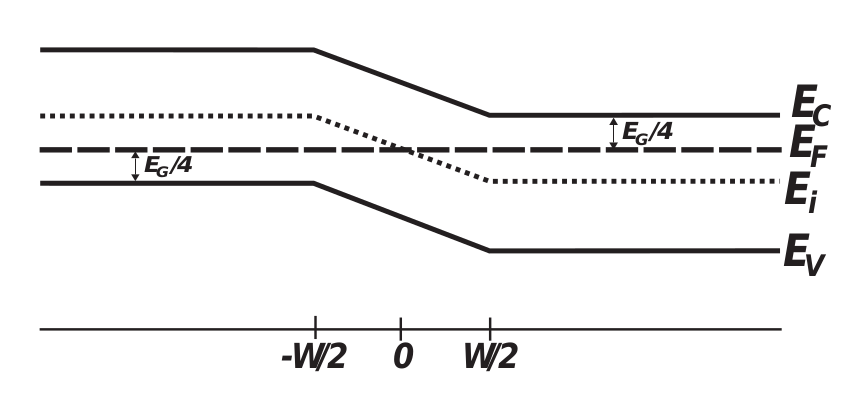
\includegraphics[width=0.7\linewidth]{Ejercicios/Ch_02/02_Ejercicio_15.png}		
\end{center}

\begin{itemize}
	\item[(a)] Si el semiconductor de Si se mantiene a temperatura ambiente, determinar la resistividad del semiconductor para la región \(x > W/2\). Para los electrones en la región \(x > W/2\) que intentan moverse a la región \(x < -W/2\) sin modificar su energía total, ¿cuál es la mínima energía cinética que deben tener?
	\item[(b)] Calcular y representar gráficamente el potencial electrostático y el campo eléctrico en función de \(x\). Explicar si el semiconductor está en equilibrio termodinámico.
	\item[(c)] Responder las siguientes preguntas:
		  \begin{itemize}
			  \item ¿Cuál es la densidad de corriente de electrones (\(J_n\)) y de huecos (\(J_p\)) en \(x = 0\)?
			  \item ¿Existe corriente de arrastre de electrones en \(x = 0\)? Si así fuera, ¿cuál es la dirección del flujo de corriente de arrastre?
			  \item ¿Existe corriente de difusión de electrones en \(x = 0\)? En tal caso, ¿cuál es la dirección del flujo de corriente de difusión?
			\end{itemize}
  \end{itemize}
\end{Enunciado}




\begin{enumerate}[label=\alph*)]
	\item La resisitividad, como hemos visto a lo largo de todos los ejericcios, viene dada por:
	\begin{equation}
		\rho = \frac{1}{q(\mu_n n + \mu_p p)}
	\end{equation}
	Por lo que solo tenemos que calcular $n$ y $p$ para $\mu_n$ y $\mu_p$ dados (valores que tendremos que coger de otro ejercicio). Así pues, obtenemos $n$ y $p$ a partir de las ecuaciones:

	\begin{equation}
		n = n_i e^{(E_F-E_i)/kT} \qquad p = n_i e^{(E_i-E_F)/kT}
	\end{equation}
	Donde conocemos $N_C$ y $N_V$ a 300K (temperatura ambiente) y la diferencia de $E_c-E_F=E_g/4$ y $E_F-E_v=3E_g/4$ en $x>W/2$ (véase diagrama de bandas). Así pues conocemos los valores:

	\begin{equation}
		n= 7.91\times 10^{14} \ \cm^{-3} \tquad p = 4.5\times 10^{14} \ \cm^{-3}
	\end{equation}
	Usando las siguientes movilidades (calculadas con las ecuacioens de portadores mayoritarios/minoritarios previas):
	
	\begin{equation}
		\mu_n = 1290 \ \cm^2 /  \text{V s} \tquad \mu_p = 499 \ \cm^2 /  \text{V s}
	\end{equation}
	tal que la resistividad en $W/2<x$:

	\begin{equation}
		\rho = 5.02 \ \Omega \cm
	\end{equation}
	\textcolor{red}{Da 7.73. En gneral hacen aproximaciones ignorando uno de los portadores.} Ahora solo queda calcualar la energía cinética mínima $T_{\min}$ que deben tener. Como podemos ver la energía de la banda de conducción aumenta de la región $x>W/2$ a la región $x<W/2$. Así pues:

	\begin{equation}
		T_{\min} = E_c(-W/2) - E_c(W/2) = E_g/2 = 0.506 \	 \eV
	\end{equation}
	\item Como sabemos el campo eléctrico viene dado por:
	\begin{equation} 
		\Ecal = \frac{1}{q} \derivadas{E_i}{x}
	\end{equation}
	y el potencial $V(x)=-E_i(x)+V_0$ donde $V_0$ es una constate arbitraria que nos ayuda a redefinir el cero del potencial. Como para calcular la derivada (y $V_0$ siempre nos permite redefinir el cero de $V$) solo necesitamos conocer la \textit{dependencia de $E_i$ con la posición}, podemos escribir 

	\begin{equation}
		E_i = E_{i0} - \frac{E_g}{2} \frac{x}{W}
	\end{equation}
	siendo $E_{i0}$ una constante irrelevante que contiene información de la energía respecto al cero $E_F=0$ eV. Así pues:

	\begin{equation}
		\Ecal = - \frac{1}{q} \frac{E_g}{2W}
	\end{equation}
	Así pues:

	\begin{equation}
		V=V_0 + \frac{E_g}{q} \frac{x}{2W} 
	\end{equation}
	Para ver si está en equilibrio termodinámico tenemos que ver si $J_n=J_p=0$. Veamos que $J_n=0$ implica que:

	\begin{equation}
		J_n = J_n |_{\text{difusion}} +J_n |_{\text{arrastre}} = q\mu_n n \Encal + qD_n\derivadas{n}{x} = 0
	\end{equation}
	De tal modo que, si estamos en equilibrio se tiene que verificar que
	\begin{equation}
		\Ecal_n = \frac{D_n}{\mu_n} \frac{1}{n} \derivadas{n}{x} = 
		\frac{kT}{q} \frac{1}{n} \derivadas{n}{x}
	\end{equation} 
	donde hemos aplicado las reglas de Einstein (válido para el equlibrio y fuera del equlibrio). Ahora solo tenemos que evaluar $n(x)$ y su derivada. Es sencillo de ver que la única dependencia mostrada en el diagrama de bandas:

	\begin{equation}
		n = \left\lbrace
		\begin{array}{ll}
			N_c e^{-\frac{1}{kT}\frac{3E_g}{4}}	& \text{si} \ x<-W/2 \\
			N_c e^{-\frac{1}{kT}\frac{E_g}{4} \parentesis{\frac{-x+W}{W/2}}}	& \text{si} \ -W/2<x<W/2 \\
			N_c e^{-\frac{1}{kT}\frac{E_g}{4}} & \text{si} \ W/2<x
		\end{array} \right.
	\end{equation}
	De lo cual deducimos que la derivada es:

	\begin{equation}
		\derivadas{n}{x} = \left\lbrace
		\begin{array}{ll}
			0	& \text{si} \ x<-W/2 \\
			\frac{1}{kT}\frac{E_g}{4}\frac{2}{W}N_c e^{-\frac{1}{kT}\frac{E_g}{4} \parentesis{\frac{-x+W}{W/2}}}	& \text{si} \ -W/2<x<W/2 \\
			0 & \text{si} \ W/2<x
		\end{array} \right.
	\end{equation}
	Consecuentemente el campo eléctrico:

	\begin{equation}
		\Ecal_n = - \frac{1}{q} \frac{E_g}{2W}   \qquad \text{si} \ - W/2<x<W/2
	\end{equation}  
	Que como podemos ver es la misma expresión. Para los portadores huecos se puede llegar a lo mismo siguiendo los mismos pasos (la única diferencia es que aparecen dos signos menos que se cancelan). Veamos como quedan las gráficas:

	\begin{center}
		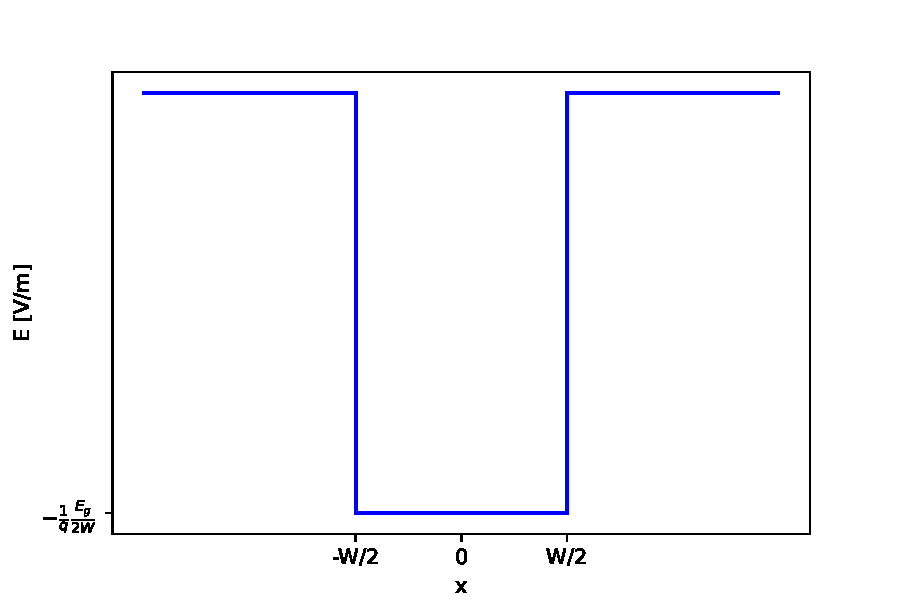
\includegraphics[width=0.7\linewidth]{Ejercicios/Ch_02/02_Ejercicio_15_E(x).pdf}
	\end{center}
	\begin{center}
		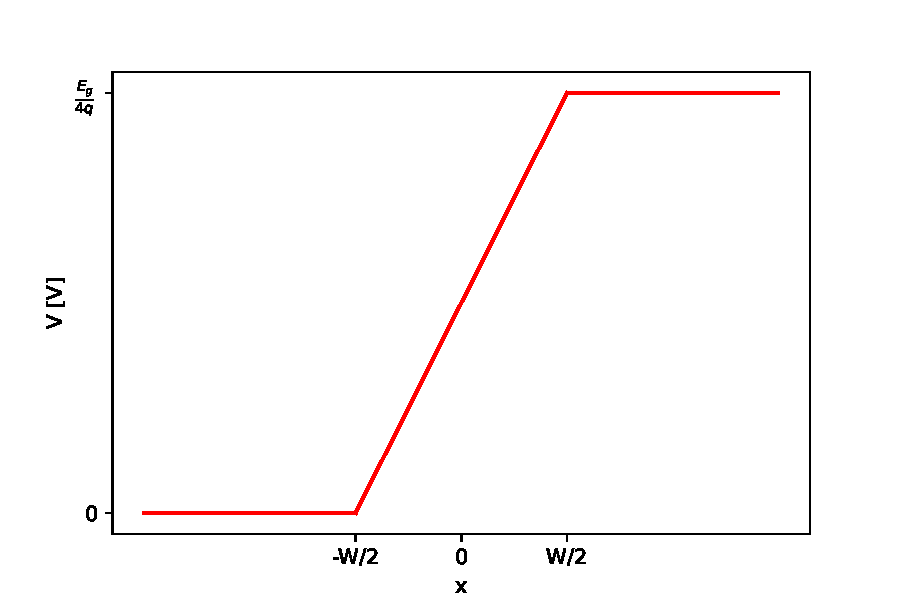
\includegraphics[width=0.7\linewidth]{Ejercicios/Ch_02/02_Ejercicio_15_V(x).pdf}
	\end{center}

	\item Respondemos a cada una de las preguntas:
	\begin{itemize}
		\item La densidad de corriente de electrones y de huecos en $x=0$ es cero, como hemos visto en el apartado anterior. De otra manera no estaríamos en el equilibrio termodinámico.
		\item Corriente de arrastre hay, ya que el campo eléctrico no es nulo (en $x=0$). Así pues: 
		\begin{equation}
			\Jn_n |_{\text{arrastre}} = q \mu_n n \Encal =  - \mu_n \frac{E_g}{2W} N_c  e^{-\frac{1}{kT}\frac{E_g}{2}}  \hnx 
		\end{equation}
		Lógicamente la corriente de arrastre tiene que tener la misma dirección que la corriente eléctrica, ya que aún que la velocidad del electrón tendrá la dirección contraria al campo eléctrico y la corriente de carga tendrá la dirección contraria a la velocidad del electrón. 
		\item Corriente de difusión hay, y en virtud de que $\Jn_n|_{\text{arrastre}}=- \Jn_n|_{\text{difusion}}$, tenemos que
		\begin{equation}
			\Jn_n |_{\text{arrastre}} = - q \mu_n n \Encal =  \mu_n \frac{E_g}{2W} N_c  e^{-\frac{1}{kT}\frac{E_g}{2}}  \hnx 
		\end{equation}
	\end{itemize}
\end{enumerate}


\begin{Enunciado}
\subsection*{Ejercicio 8}

Interpretación de un diagrama de bandas de energía para un semiconductor de silicio tomando $L=1$ micra:
\begin{center}
	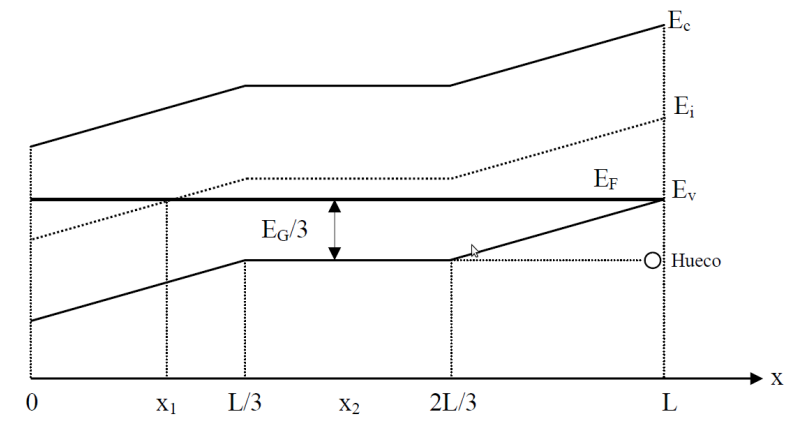
\includegraphics[width=0.7\linewidth]{Ejercicios/Ch_02/02_Ejercicio_16.png}		
\end{center}
\begin{itemize}
	\item[(a)] Calcula y representa graficamente el potencial electrostático y el campo eléctrico en el interior del semiconductor. Determina si el sistema esta o no en equilibrio termodinámico.
	\item[(b)] Calcula si el semiconductor es degenrado en alguna zona. En $x=x_2$, ¿a qué es igual $p$?
	\item[(c)] Captura la densidad de corriente de electrones $J_n$ y la densidad de corriente de arrastre de huecos $J_p^a$ que fluye en $x=x_1$. Determina cuanto vale la energía cinética del hueco que aparece en el diagrama en la posición $x=L$. 
\end{itemize}

\end{Enunciado}




\begin{enumerate}[label=\alph*)]
	\item Queremos calcular el potencial electrostático y el campo eléctrico en el interior del semiconductor. Usamos la misma relación que en el ejercicio anterior:
	\begin{equation}
		\Ecal = \frac{1}{q} \derivadas{E_i}{x}
	\end{equation}
	Veamos que la energía varía como:
	\begin{equation}
		E_i(x) = \left\lbrace \begin{array}{ll}
			\frac{E_{i0}}{L/3-x_1} (x-x_1) \quad & \ \text{si} \ x<L/3 \\
			E_{i0} \quad & \ \text{si} \ L/3<x2L/3 \\
			E_{i0+\frac{E_{i0}}{L/3-x_1} (x-2L/3)} \quad & \ \text{si} \ 2L/3<x
		\end{array} \right.
	\end{equation}
	Recordamos que en $L/3$ tenemos que $E_v=-E_g/3$, y por tanto $E_c=2E_g/3$, tal que $E_{i0}=E_g/6+(3kT/4)\cdot \log(m_n^*/m_p^*)=0.179 \ \eV$, donde hemos redefinido $E_F=0$. Por lo que igual que antes tenemos que el campo eléctrico viene dado por regiones:
	\begin{equation}
		\Ecal(x) = \left\lbrace \begin{array}{ll}
			\frac{E_{i0}}{L/3-x_1} \quad & \ \text{si} \ x<L/3\\
			0 \quad & \ \text{si} \ L/3<x2L/3 \\
			\frac{E_{i0}}{L/3-x_1} \quad & \ \text{si} \ 2L/3<x
		\end{array} \right.
	\end{equation}
	y por tanto:

	\begin{equation}
		V(x) = \left\lbrace \begin{array}{ll}
			V_0 -\frac{E_{i0}}{L/3-x_1} (x-L/3) \quad & \ \text{si} \ x<L/3 \\
			V_0 \quad & \ \text{si} \ L/3<x2L/3 \\
			V_0 -\frac{E_{i0}}{L/3-x_1} (x-2L/3) \quad & \ \text{si} \ 2L/3<x
		\end{array} \right.
	\end{equation}
	Ahora solo tendríamos que hacer el esquema:

	\begin{center}
		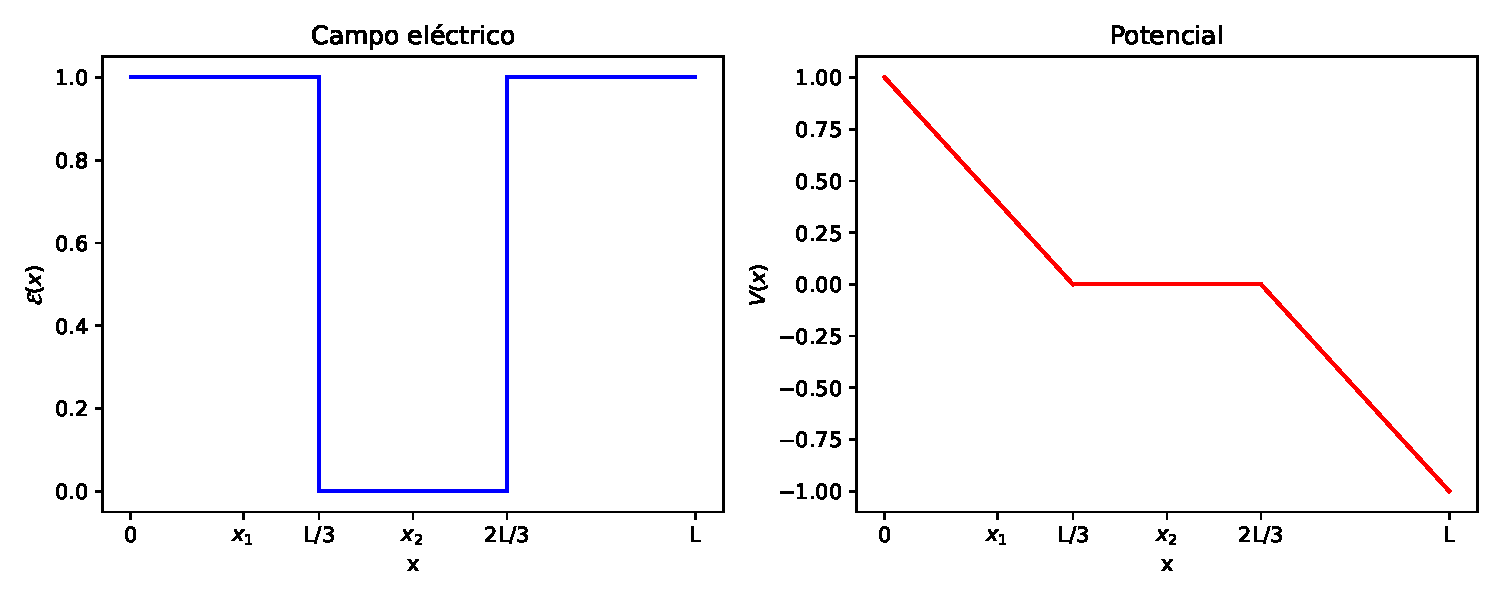
\includegraphics[width=\linewidth]{Ejercicios/Ch_02/02_Ejercicio_16.pdf}
	\end{center}
		
	Para determinar que está en equilibrio basta ver que $\Jn_T=0$ y que $T=\cte$, lo cual es cierto. Para ver que $\Jn=0$ debemos seguir el mismo procedimiento que antes.
	\item  Evidentemente es degenerado en $x=L$, ya que $E_F=E_v$. En $x_2$ tenemos que: 
	\begin{equation}
		p = N_V e^{\frac{E_F-E_v}{kT}} = N_V e^{\frac{E_g}{3kT}} = n_i e^{\frac{E_F-E_i}{kT}}
	\end{equation}
	tal que en $x_2$ tenemos que $E_i=E_{i0}=0.179 \ \eV$. Los datos:

	\begin{equation}
		p = 1.22 \times 10^{13} \ \cm^{-3}
	\end{equation}
	\item Nos piden la densidad de corriente de electrones $J_n$ y la densidad de corriente de huecos en $x=x_1$. Es exactamente igual que en el anterior ejercicio:
	\begin{equation}
		\Jn|_{\text{{arrastre}}} = q \mu_n n \Encal = 0
	\end{equation}
	ya que en $x_1$ no hay corriente. La energía cinética del hueco $T$ viene dada por la diferencia entre $E_v=0$ (en $x=L$) y $-E_g/3$. Así pues:

	\begin{equation}
		T = - \frac{-E_g}{3}
	\end{equation}
	por suponer, ya que no tenemos ningún tipo de motivación para suponer que es así. 

\end{enumerate}









\chapter{Reacciones Nucleares}

Las reacciones nuclares más comunes tienen lugar cuando una partícula enegética incide sobre un núcleo y éste se transforma: exictándose, rompiéndose o simplemente absorbiendo la partícula incidente. Estas partículas incidentes son generalmente neutrones, protones, partículas $\alpha$ o fotones $\gamma$. Para que penetren dentro de del núcleo sobre el que inciden es necesario que lleven cierta energía. En la Tierra esa energía se puede conseguir con aceleradores o reactores nucleares, y también a partri de fuentes naturales radiactivas. Las reacciones nucleares permiten el estudio de las interacciones que gobiernan el mundo subnuclear y, por otro lado, proporcionan la mayor parte de los datos tabulados sobre las propiedades nucleares. Estas dos cosas, están obviamente relacionadas, porque sólo es posible entender las propiedades de los núcleos, si se posee al mismo tiempo una buena comprensión de las interacciones nucleares.

% Faltan cosas

\section{Tipos de reacciones}

Representamos una reacción nuclear típica de las siguientes dos maneras equivalentes:

\begin{equation}
    a + A  \longrightarrow B + b \tquad A(a,b)B \label{Ec:03-01-01}
\end{equation}
donde $a$ es el proyectil o partícula acelerada que se hace incidir sobre el núcleo blanco, $A$, en reposo en el sistema laboratorio. De las partículas en el segundo miembro de la reacción, $B$ suele ser un núcleo pesado que no abandona el material del blanco, y $b$ una partícula para referirse a un conjunto de reacciones del mismo tipo. Así diríamos reacciones ($\alpha,n$) o ($n,\gamma$), por ejemplo. Hay muchas maneras de clasificar las reacciones nucleares. He aquí unas cuantas:

\begin{itemize}
    \item Se suele hablar de una \textbf{reacción de dispersión} (\textit{scattering process}) cuando las partículas iniciales y finales son las mismas\footnote{En física de partículas de altas energías se usa el término \textit{scattering} de un modo más general, no sólo para referirse a reaccioens en las que las partículas iniciales coinciden con las finales. En el \textit{deep inelastic scattering} por ejemplo, la energía del proyectil es tan alta que se producen muchas partículas en el estado final}. La dispersión puede ser \textbf{elástica} si las patículas o núcleos $B$ y $b$ se encuentran en su estado fundamental, o \textbf{inelástica} si alguna de las dos queda en un estado excitado, que posteriormente se suele desexcitar por emisión gamma. En una dispersión elástica la energía cinética se conserva ($Q=0$) y simplemente se redistribuye entre las partículas interaccionantes.
    \item Si las partículas $a$ y $b$ son la misma, y además tenemos otro nucleón en el estado final (3 partículas como productos) se suele denominar una \textbf{reacción knockout}.
    \item Tenemos una \textbf{reacciones de transferencia} (\textit{transfer reaction}) cuando se transfieren uno o varios nucleones entre el proyectil y el blanco.
\end{itemize}

% Faltan cosas


\section{Leyes de conservación}

\subsection{Conservación de la carga eléctrica y el número bariónico}

Aunque veremos en un capítulo posterior estas leyes de conservación con algo más de detalle, conviene mencionarlas ya aquí. La carga eléctrica total de las partículas iniciales de la reacción es siempre igual a la de las partículas finales. La \textbf{conservación de la carga eléctrica} es una ley \textit{muy fundamental} en nuestro entendimiento actual de la física, al mismo nivel que la ley de conservación de la energía.

% Insertar foto tikz

Si asginamos a cada a cada barión\footnote{Un barión es un hadrón (partícula sensible a la interacción fuerte) con espín semientero. Los bariones más ligeros son los familiares protón y neutrón.} una unidad positiva de \textit{número bariónico} y a cada antibarión una unidad negativa, podemos formular una ley de \textbf{conservación del número de bariónico} en cualqueir reacción diciendo que la suma de números bariónicos para las partículas iniciales debe coincidir con la misma suma para las partículas finales.  % Falta texto

\subsection{Conservación de la energía y del momento lineal}

Las interacciones nucleares tienen lugar a distancia mucho más pequeñas que la separación típica entre los núcleos de un material ordinario, por eso se puede considerar a las partículas interaccionantes en una reacción nuclear como un sistema aislado y aplicar la ley de conservación de la energía total y del momento lineal total. De acuerdo con la notación expresada en (\ref{Ec:03-01-01}) escribimos la \textbf{conservación de la energía}

\begin{equation}
    T_a + m_a c^2 +T_A+m_A c^2 = T_b +m_bc^2 + T_b + m_Bc^2
\end{equation}
tal que $E_A = T_A + m_Ac^2$... El valor $Q$ del proceso o de la reacción se define como la difernecia entre la energía cinética inicial y final 

\begin{equation}
    Q \equiv T_B + Tb - T_A - T_a = (m_A + m_a - m_B - m_b) c^2
\end{equation}

Si, como es habitual, estamos analizando un experimento en el que el núcleo blanco se encuentra en reposo en el sistema laboratorio ($T_A=0$), entonces tenemos que $Q = T_B + T_b - T_a$. La energía cinética del núcleo $T_B$ es dfifícil de medir, y son las energías del proyectil y la de la partícula emergente ($T_a$ y $T_b$) las que suelen medirse. La De todos modos veremos que podemos encontrar una expresión para $Q$ (ecuación ())  que no incluye la energía cinética.


% Falta texto

\subsection{Energía umbral de reacción}

\subsection{Conservación del moemnto angular y de la paridad}

\subsection{Isospín}

\section{Dispersión y secciones eficaces}

Lo que usualmente se mide en las reacciones nucleares es el momento de las partículas ligeras emitidas (y por lo tanto su energía cinética, supuesto que se conozca la identidad de la partícula) y su distribución angular. % Falta texto

\subsection{Atenuación de un haz al atravesar un blanco}


\subsection{Dispersión de Coulomb}

\subsection{Dispersión nuclear}


\section{Mecanismos de reacciones}

\section{Fisión}

\section{Fusión}

La mayor dificultad para lograr la fusión nuclear a gran escala consiste en mantener el material fusible confinado a altas temperaturas durante el tiempo suficiente. Hasta el momento se está investigando en dos métodos: el confinamiento magnético y el confinamiento inercial. En el primero se hace circular plasma caliente de núcleos $^2$H y $^3$H en una región confinada por campos electromagnéticos. En el segundo se inyecta luz láser en una pequeña región que contiene el material fusible. En cualquier caso, el aprovechamiento comercial de la energía de fusión parece todavía una posibilidad lejana.

\section{Apéndices}
\newpage

%%%%%%%%%%%%%%%%%%%%%%%%%%%%%%%%%%%%%%%%%%%%%%%%%%%%%%%%%%%%%%%%%%%%%%%
%%%%%%%%%%%%%%%%%%%%%%%%%%%%%%%%%%%%%%%%%%%%%%%%%%%%%%%%%%%%%%%%%%%%%%%
%%%%%%%%%%%%%%%%%%%%%%%%%%%%%%%%%%%%%%%%%%%%%%%%%%%%%%%%%%%%%%%%%%%%%%%
%%%%%%%%%%%%%%%%%%%%%%%%  EJERCICIOS %%%%%%%%%%%%%%%%%%%%%%%%%%%%%%%%%%
%%%%%%%%%%%%%%%%%%%%%%%%%%%%%%%%%%%%%%%%%%%%%%%%%%%%%%%%%%%%%%%%%%%%%%%
%%%%%%%%%%%%%%%%%%%%%%%%%%%%%%%%%%%%%%%%%%%%%%%%%%%%%%%%%%%%%%%%%%%%%%%
%%%%%%%%%%%%%%%%%%%%%%%%%%%%%%%%%%%%%%%%%%%%%%%%%%%%%%%%%%%%%%%%%%%%%%%

\newpage

\section*{Ejercicios}
\addcontentsline{toc}{section}{\textit{Ejercicios}}

%%%%%%%%%%%%%%%%%%%%%%%%%%%%%%%%%%%%%%%%%%%%%%%%%%%%%%%%%%%%%%%%%%%%%%%
%%%%%%%%%%%%%%%%%%%%%%%%% EJERCICIOS 1 %%%%%%%%%%%%%%%%%%%%%%%%%%%%%%%%
%%%%%%%%%%%%%%%%%%%%%%%%%%%%%%%%%%%%%%%%%%%%%%%%%%%%%%%%%%%%%%%%%%%%%%%

\begin{Enunciado}
\subsection*{Ejercicio 1}

Queremos estudiar las características de una unión abrupta PN de silicio a temperatura ambiente con boro (\(10^{15} \, \text{cm}^{-3}\)) y fósforo (\(5,0 \times 10^{14} \, \text{cm}^{-3}\)), siendo la longitud de la zona P de \(0,008 \, \text{cm}\) y la de la zona N de \(0,008 \, \text{cm}\) y el área del contacto de \(10^{-2} \, \text{cm}^2\). 

Las movilidades de electrones y huecos son \(1360 \, \text{cm}^2/(\text{V}\cdot\text{s})\) y \(460 \, \text{cm}^2/(\text{V}\cdot\text{s})\) respectivamente y \(\tau_p = \tau_n = 10^{-6} \, \text{s}\).

\begin{enumerate}[label=\alph*)]
\item En situación de equilibrio, calcula y representa lo siguiente:
\begin{itemize}
    \item La anchura de todas las regiones del dispositivo.
    \item Las bandas de energía incluyendo la banda de conducción, la de valencia, el nivel de Fermi, y el de Fermi intrínseco. Calcula la distancia relativa entre todos esos niveles.
\end{itemize}

\item Si polarizamos la zona N con 0,2 voltios respecto a la zona P, calcula y representa:
\begin{itemize}
    \item La anchura de todas las regiones del dispositivo.
    \item Las bandas de energía incluyendo la banda de conducción, la de valencia, el nivel de Fermi, y el de Fermi intrínseco. Calcula la distancia relativa entre todos esos niveles.
\end{itemize}

\item Si polarizamos la zona N con 0,2 voltios respecto a la zona P, calcula y representa:
\begin{itemize}
    \item El campo eléctrico, densidad de carga y el voltaje en todo el dispositivo.
    \item Las corrientes que surgen a lo largo de todo el dispositivo para cada portador.
\end{itemize}
\end{enumerate}
\end{Enunciado}


Vamos a calcular las masas efectivas en función de las movilidades y las vidas medias:

\begin{equation}
    \mu_n = D_n \frac{q}{kT} = \frac{q}{kT} \tau_n v^2_{th} = \frac{q}{kT} \tau_n \frac{3kT}{m_n^*} = \frac{3q\tau_n}{m_n^*}
\end{equation}
Entonces:
\begin{equation}
    m_n^* = \frac{3q\tau_n}{\mu_n} \qquad m_p^* = \frac{3q\tau_p}{\mu_p^*}
\end{equation}
Usando estas ecuacioens obtenemos:

\begin{equation}
    m_p^* = 3.88 \cdot 10^6 \ m_e \tquad m_n^* = 11.5 \cdot 10^6 \ m_e
\end{equation}
Francamente no se que puede estar mal, pero usaremos las masas típicas $m_p^* = 0.81m_e$ y $m_n=1.18 m_e$. 
\begin{enumerate}[label=\alph*)]
    \item Tenemos que calcular la anchura de todas las regiones del dispositivo y las bandas de energía (banda de conducción, banda de valencia, nivel de Fermi y nivel de Fermi intrínseco). También tenemos que calcular las distancias relativas entre los niveles (lo cual es obvio dado lo anterior). 
    
    Primero tenemos que calcular las distancias, lo cual es simplemente aplicar las fórmulas para la situación de equilibrio
    \begin{equation}
        x_p = \ccorchetes{\frac{2K_S\varepsilon_0}{q} \frac{N_D}{N_A(N_A+N_D)}  V_{bi}}^{1/2}  \qquad 
        x_n = \ccorchetes{\frac{2K_S\varepsilon_0}{q} \frac{N_A}{N_D(N_A+N_D)}  V_{bi}}^{1/2}
    \end{equation}
    Así pues, los valores numéricos son: 

    \begin{equation}
        x_p = 5.000\cdot 10^{-5}  \ [\cm] \qquad x_n =1.000\cdot 10^{-4}  \ [\cm] \qquad W = x_n + x_p = 1.5 \cdot 10^{-4} \ [\cm ]
    \end{equation}
    Y luego tenemos que calcular los valores de todas y cada una de las bandas. Para conocer las banda, teniendo en cuenta que $E_F=0 \ [\eV]$  \textit{a lo largo de todo el dispositivo pn}. Por el resto simplemente aplicar las ecuaciones de la sección 2, tal que en la zona $p$ los valores son los que típicamente esperaríamos para un semiconductor $N_A$, mientras que en la zona $n$ será los que esperaríamos en un conductor $N_A$ menos $V_{bi}$. En la \textit{zona de vaciamiento} los valores de las bandas simplemente valdrán su valor en $p$ menos el valor $V(x)$:
    \begin{equation*}
        V_{bi} = \frac{kT}{q} \ln \parentesis{\frac{N_AN_D}{n_i^2}} = 0.580 \ [\unit{V}]
    \end{equation*}
    \begin{equation*}
        V(x) = \left\lbrace \begin{array}{ll}
            - \frac{qN_A}{2K_S\varepsilon_0} \parentesis{x_p + x}^2  & \ - x_p \leq x \leq 0 \\
            - \frac{qN_D}{2K_S\varepsilon_0} \parentesis{x_n - x}^2 + V_{bi}  & \ 0 \leq x \leq x_n \\
        \end{array} \right.
    \end{equation*}
    Por el resto de situaciones, tenemos que en la zona $p$ las ecuaciones son:
    \begin{equation*}
        E_i = - kT \ln \parentesis{\frac{n}{n_i}} = kT \ln \parentesis{\frac{N_A}{n_i}} \qquad E_c  = E_i  + kT \ln \parentesis{\frac{N_c}{n_i} } \qquad E_v  =E_c-E_g
    \end{equation*}
    tal que 
    \begin{equation*}
        E_g = 1.12 \ [\eV] \qquad N_C = 2 \parentesis{\frac{m_n^* kT}{2\pi \hbar^2}}^{3/2}  = 3.21 \cdot 10^{19} \ [\cm^{-3}] \end{equation*}
    \begin{equation*}    
       N_V = 2 \parentesis{\frac{m_p^* kT}{2\pi \hbar^2}}^{3/2} = 1.83 \cdot 10^{19} \ [\cm^{-3}] 
    \end{equation*}
    \begin{equation*}
        n_i = \sqrt{N_CN_V} e^{-E_g/2kT} = 9.49 \cdot 10^9 \ [\cm^{-3}]
    \end{equation*}
    Así pues obtenemos los siguientes resultados numéricos: 
    \begin{center}
        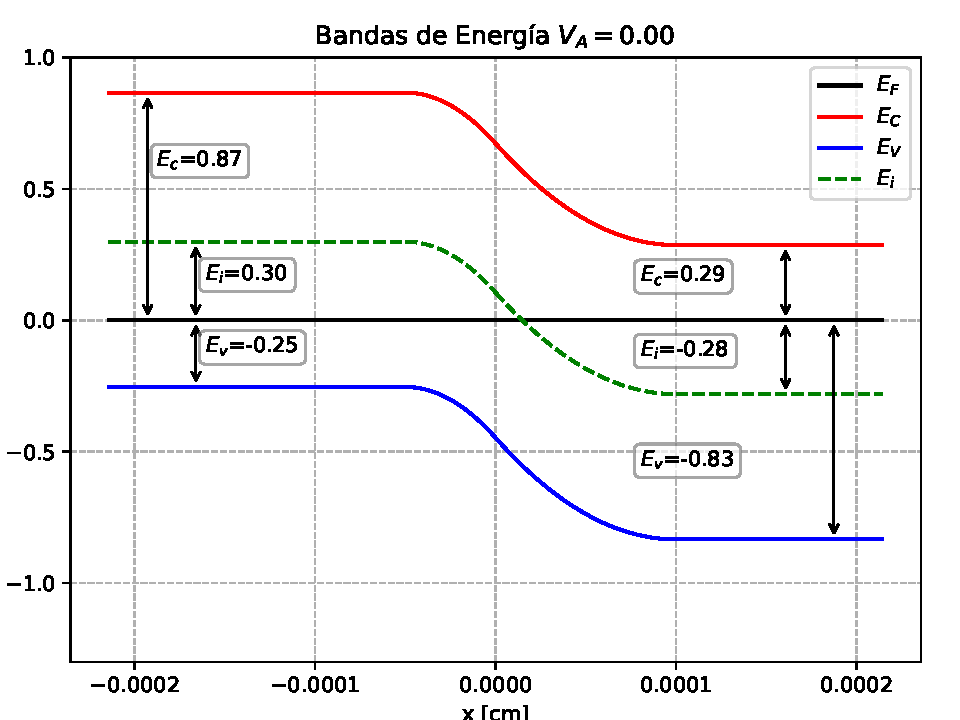
\includegraphics[width=0.85\linewidth]{Ejercicios/Ch_03/03_01_Bandas.pdf}
    \end{center}
    \item Si polarizamos la zona N con 0.2 voltios ($V_A=-0.2$V) estamos en el régimen de polarización inversa. El calculo de los anteriores valores es exáctamente igual solo que ahora tenemos que $V_{bi}\rightarrow V_{bi}-V_A$. Así pues:
    \begin{equation}
        x_p = 5.79867 \cdot 10^{-5}  \ [\cm ] \tquad
        x_n = 1.15973 \cdot 10^{-4}  \ [\cm ]
    \end{equation}
    \begin{center}
        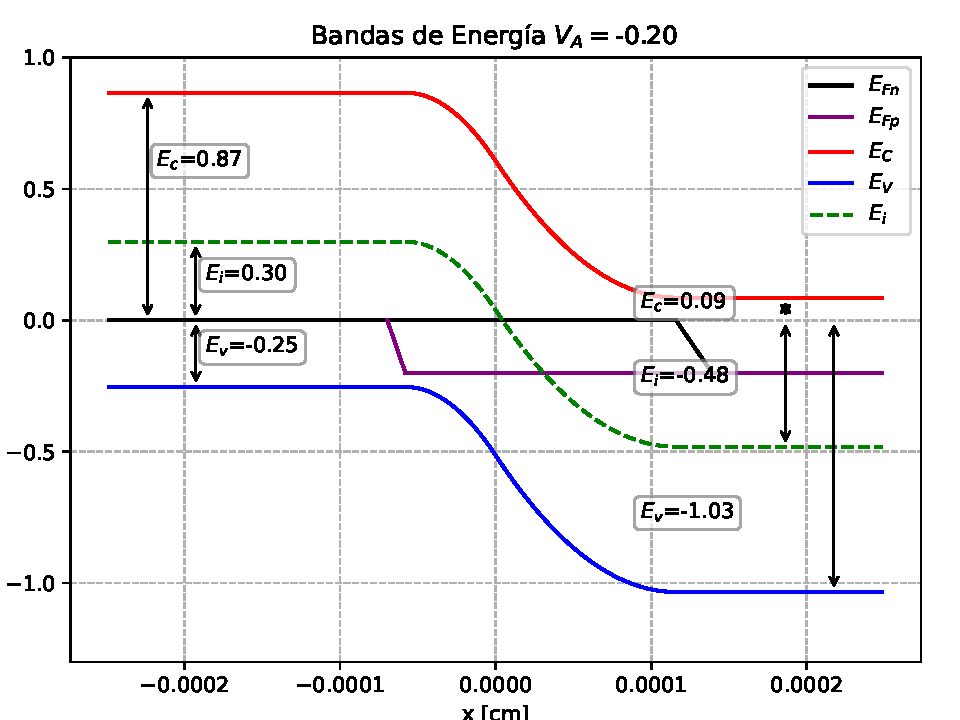
\includegraphics[width=0.7\linewidth]{Ejercicios/Ch_03/03_02_Bandas.pdf}
    \end{center}

    \item Ahora nos piden calcular el campo eléctrico, la densidad de carga y el voltaje a lo largo del dispositivo, así como las corrientes a lo largo del mismo. Para calcular el campo eléctrico tenemos que usar la típica fórmula:

    \begin{equation}
        \Ecal = - \derivadas{V}{x} = \frac{1}{q} \derivadas{E_i}{x}
    \end{equation}
    Así por lo tanto tenemos que: 

    \begin{equation*}
        \Ecal(x) = \left\lbrace \begin{array}{ll}
            - \frac{qN_A}{K_S\varepsilon_0} \parentesis{x_p - x}  & \ - x_p \leq x \leq 0 \\
            - \frac{qN_D}{K_S\varepsilon_0} \parentesis{x_n - x} & \ 0 \leq x \leq x_n \\
        \end{array} \right.
    \end{equation*}
    siendo 0 en el resto de puntos del dispositvo. El volaje se calcula teniendo en cuenta la anterior ecuación (considerando que el cero del potencial está en la zona $p$) on la ecuación que hemos usado previamente (a). Solo falta calcular la densidad de carga, que se hace usando, por ejemplo, la ecuación de Maxwell

    \begin{equation}
        \nabla \cdot E = \frac{\rho}{K_S \varepsilon_0} 
    \end{equation}
    de tal modo que:

    \begin{equation}
        \rho (x) = \left\lbrace \begin{array}{ll}
            - q N_A   & \ - x_p \leq x \leq 0 \\
            q N_D \parentesis{x_n - x} & \ 0 \leq x \leq x_n \\
        \end{array} \right.
    \end{equation}
    Lo cual es en realidad trivial o directo, ya que procede de las hipótesis de vaciamiento que usamos para deducir todas las ecuaciones (en las condiciones que exigimos para la verificación de todas estas ecuaciones incluye que $n_n,p_p\ll N_D,N_A$) de tal modo que la ecuación de la carga es la primera condición, no la última. En cualquier caso, hacemos las representaciones gráficas:   
    \begin{figure}[h!]
    \centering
    \begin{subfigure}{0.47\textwidth}
        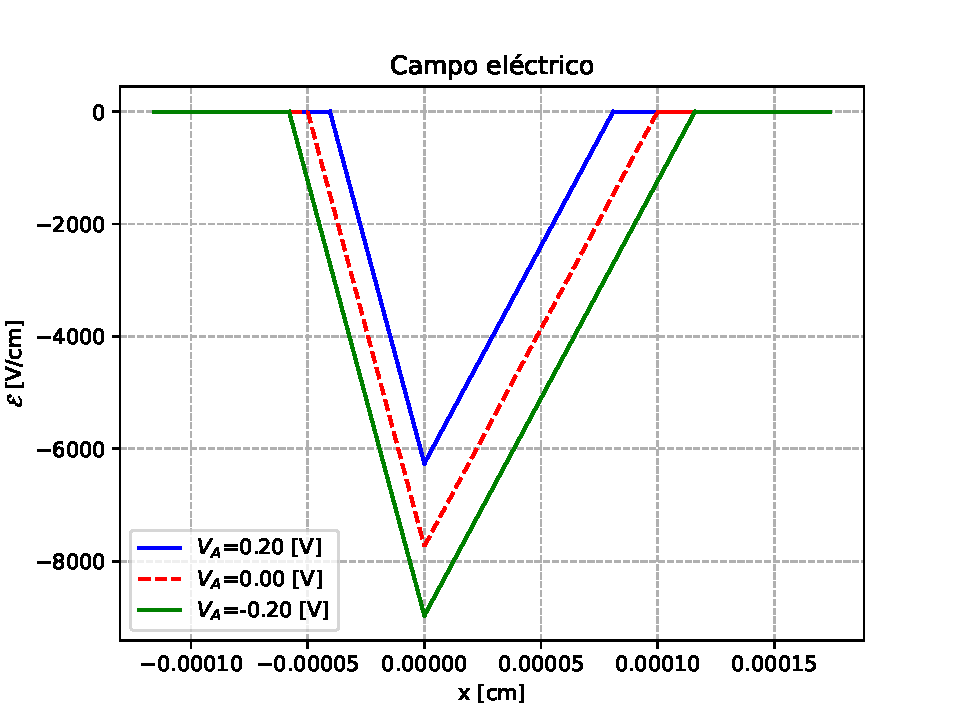
\includegraphics[width=\textwidth]{Ejercicios/Ch_03/03_04_E.pdf}
    \end{subfigure}
    \begin{subfigure}{0.47\textwidth}
        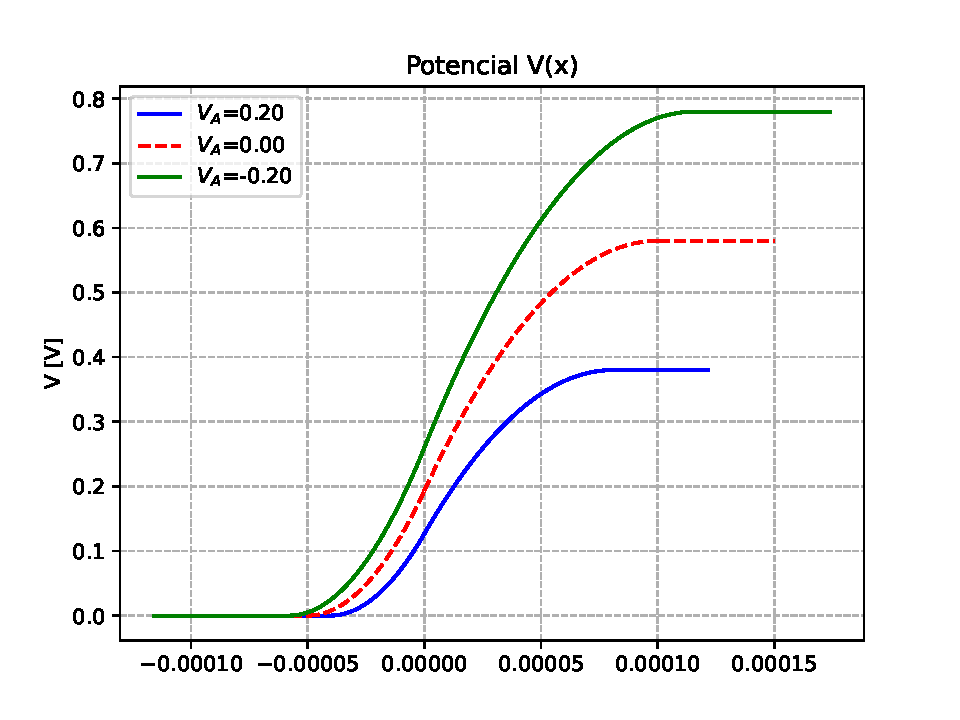
\includegraphics[width=\textwidth]{Ejercicios/Ch_03/03_05_V.pdf}
    \end{subfigure}
    \end{figure}
    \begin{center}
        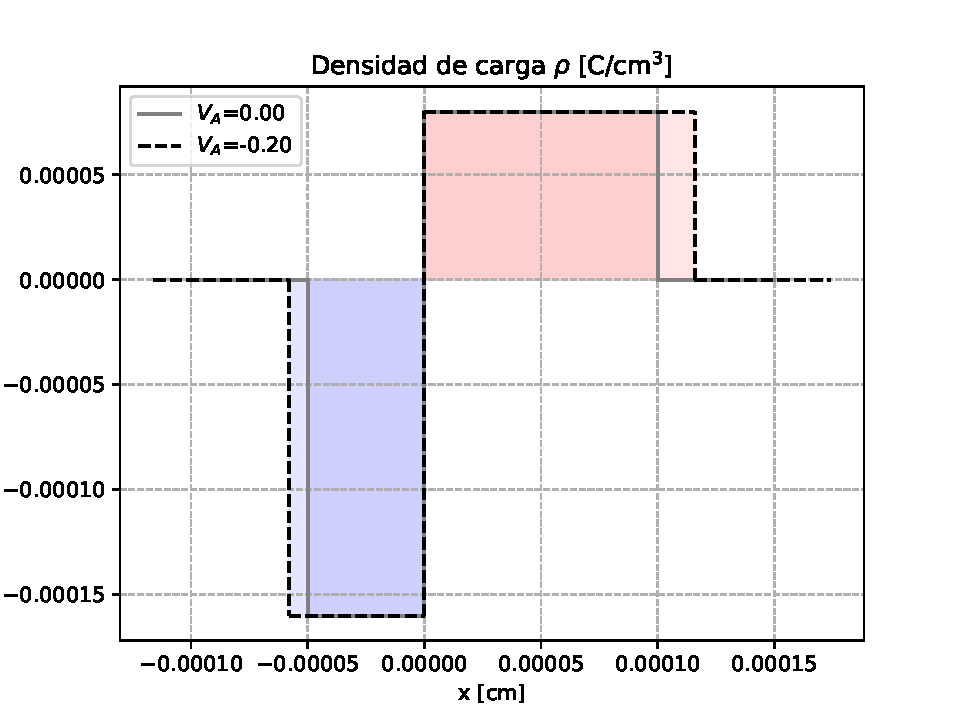
\includegraphics[width=0.6\linewidth]{Ejercicios/Ch_03/03_06_rho.pdf}
    \end{center}   
    Ahora tenemos que calcular las corrientes a lo largo del dispostivo. Las corrientes de cada portador dependen (al menos la forma funcional) depende principalmente de si nos encontramos en la región maiva $N/P$ o en la región de vaciamiento. 
    Los valroes más relevantes son aquellos que se dan en $x_n$ y $x_p$, ya que definen los valores tanto en la zona masiva como los valores en la zona de vaciamiento. Así pues, tenemos:

    \begin{equation}
        I_N (-x_p) = \frac{AqD_N}{L_N}  \frac{n_i^2}{N_A} \parentesis{e^{qV_A/kT}-1} \qquad
        I_P (x_n) = \frac{AqD_P}{L_P} \frac{n_i^2}{N_D}  \parentesis{e^{qV_A/kT}-1}
    \end{equation}
    que numéricamente se expresa como:
    \begin{equation}
        I_N (-x_p) = -8.55\cdot10^{-13} \ [\unit{A}] \qquad 
        I_P (x_n) = -9.95 \cdot 10^{-13}\ [\unit{A}]
    \end{equation}
    donde hemos usado que:

    \begin{equation}
        D_N = 35.1 \ [\unit{cm^2/s}] \quad 
        D_P = 11.9 \ [\unit{cm^2/s}] \quad L_N = 5.92 \cdot 10^{-3} \ [\cm] \end{equation}
    \begin{equation}     
        L_P = 3.45 \cdot 10^{-3} \ [\cm]  \quad n_i = 9.49 \cdot 10^{9} \ [\cm^{-3}]
    \end{equation}
    Veamos que la corriente total es:    

    \begin{equation}
        I = I_0 \parentesis{e^{qV_A/kT}-1} = I_N (-x_p) + I_P (x_n) \qquad  I_0 =  A q \parentesis{\frac{D_N}{L_N} n_{p0} + \frac{D_P}{L_P} p_{n0}}
    \end{equation}
    Con un resultado numérico de: 

    \begin{equation}
        I =  18.5 \cdot 10^{-13} \ [\unit{A}]
    \end{equation}
    Al tener un $L_N$ y $L_P$ bastante alto (de hecho del orden del tamaño del diodo) es normal que la representación gráfica sea bastante mala, y que no seamos capaces de ver esa tendencia a cero y a $I_T$ de $I_N$ e $I_P$. Usando las ecuaciones del diodo estrecho obtenemos los siguientes valores numéricos: 

    \begin{equation}
        I_N(x_p)=\SI{-9.804e-13}{[A]} \qquad  
        I_P(x_n)=\SI{-1.015e-12}{[A]} 
    \end{equation}
    \begin{equation}
        I = \SI{-1.995e-12}{[A]}
    \end{equation}
    Con la siguiente representación gráfica:
    \begin{center}
    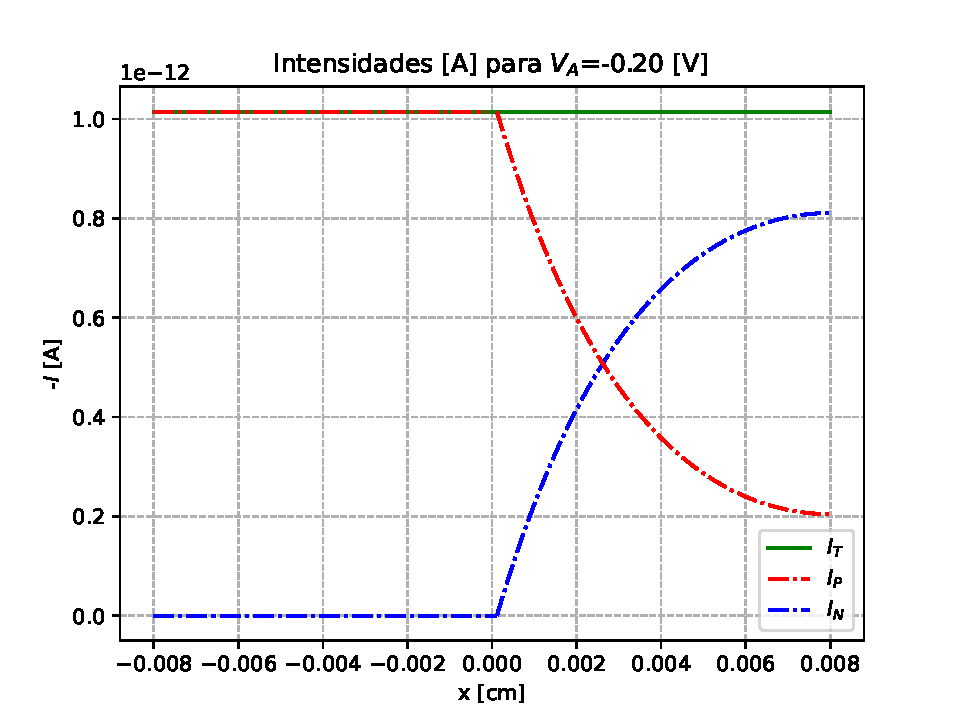
\includegraphics[width=0.6\linewidth]{Ejercicios/Ch_03/03_07_I.pdf}
    \end{center}

\end{enumerate}    
%%%%%%%%%%%%%%%%%%%%%%%%%%%%%%%%%%%%%%%%%%%%%%%%%%%%%%%%%%%%%%%%%%%%%%%
%%%%%%%%%%%%%%%%%%%%%%%%% EJERCICIOS 2 %%%%%%%%%%%%%%%%%%%%%%%%%%%%%%%%
%%%%%%%%%%%%%%%%%%%%%%%%%%%%%%%%%%%%%%%%%%%%%%%%%%%%%%%%%%%%%%%%%%%%%%%

\begin{Enunciado}
\subsection*{Ejercicios 2}

Partimos de una unión escalón NP realizada con un cristal semicondcutor de germanio ($E_G = 0.66 \ \eV$, $m_e^*=0.5$, $m_h^* = 0.37$) con $N_D=10^{16} \ \cm^{-3}$ y $N_A = 10^{15} \ \cm^{-3}$, en cada zona siendo la longitud de la zona $N$ de 0.003 cm y la de la zona P de 0.002 cm y el área de $10^{-2} \ \cm^2$. La permitividad para el germanio es de $1.4337 \times 10^{-12}$ F/cm, y el $n_i=2.0 \times 10^{13}$ cm$^{-3}$, las movilidades de electrones y huecos son $3900$ cm$^2$/(V$\cdot$s) y $1900$ cm$^2$/(V$\cdot$s) respectivamente y $\tau_n=\tau_p=10^{-6}$ s.

\begin{enumerate}[label=\alph*)]
    \item Para la situación de equilibrio, comprobar que no esté degenerado y calcular el potencial de contacto, el ancho de la región de vaciamiento y el campo eléctrico máximo.
    \item Calcula los incrementos de los portadores minoritarios en los bordes de las zonas de vaciamiento para los voltajes -0.1 y 0.1. Representa gráficamente la distribución de los portadores minoritarios e indica razonadamente si se podría aplicar la hipótesis de bajo nivel de inyección para esas polarizaciones.
    \item Calcula la corriete total y las componentes de corriente de electrones y huecos en la zona de vaciamiento para esas polarizaciones. Indica además la relación entre ellas. Representa gráficametne como varían las corrientes de electrones y huecos a lo largo de todo el dispositivo. 
\end{enumerate}
\end{Enunciado}


\begin{enumerate}[label=\alph*)]
    \item Para la situación de equilibrio comprobar que no está degenerado es sencillo, aunque necesitamos conocer la temeratura. La temperatura que tiene que haber para que nuestro gap sea $E_g=0.66\eV$ es de aproximadamente $\sim 310$K. ¿Cómo sabemos esto? Pues aplicando la ecuación de Varshini pero a la inversa. Nosotros usaremos $300$K ya que es la temperatura que usamos en todos los ejercicios, y tampoco dista mucho de la temperatura real. Así pues, para 300K, veamos que no está degenerado ya que en la gráfica: 
    \begin{center}
        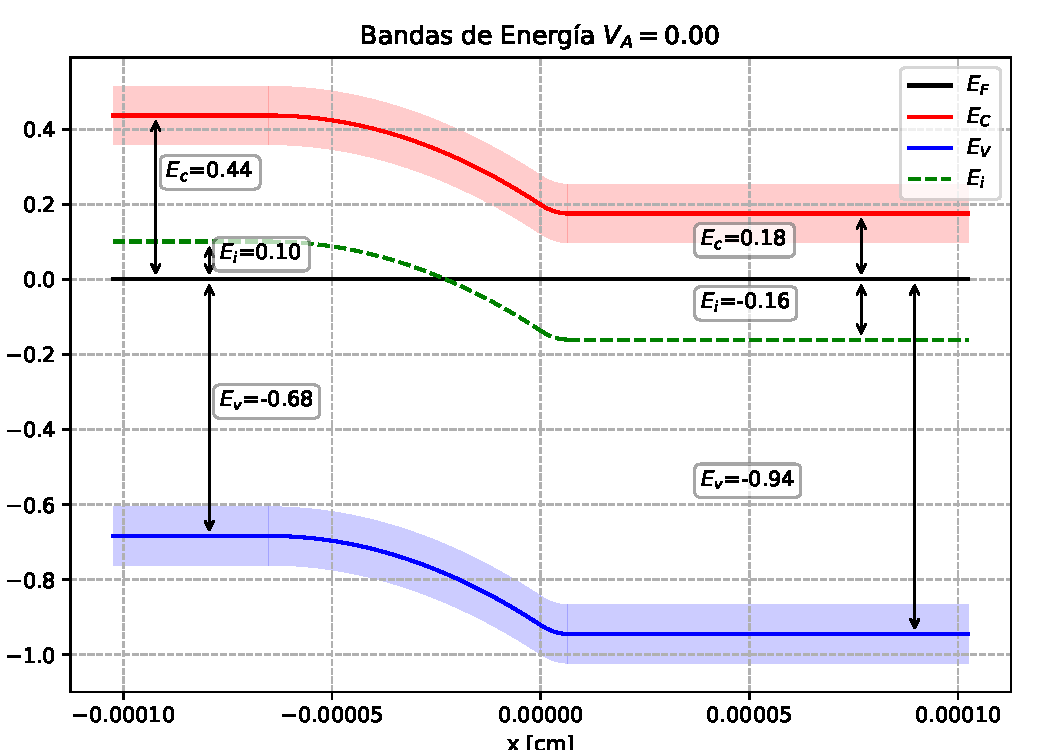
\includegraphics[width=0.6\linewidth]{Ejercicios/Ch_03/03_08_Bandas.pdf}
    \end{center}
    tal que $3k_B\cdot 300=0.078 \ \eV$. Estamos lejos de que esté degenerado. Así pues: 

    \begin{equation}
        \Vbi = 0.26 \eV \qquad x_p=6.51871 \cdot 10^{-5} \ [cm] \qquad 
        x_n= 6.51871 \cdot 10^{-6} \ [cm]
    \end{equation}
    El campo eléctrico máximo por otro lado: 

    \begin{equation}
        \Ecal_{\max}=-7284.73 \ [\unit{V/cm}]
    \end{equation}
    que se deduce de la ecuación 
    \begin{equation}
        \Ecal = - \frac{qN_A}{K_S\varepsilon_0} x_p = - \frac{qN_D}{K_S\varepsilon_0} x_n
    \end{equation}
    \item  Los incrementos de portadores minoritarios en los bordes de las zonas viene dado por:
    \begin{equation}
        \Delta n = \frac{n_i^2}{N_A} \parentesis{e^{qV_A/kT}-1}  \tquad 
        \Delta p = \frac{n_i^2}{ND} \parentesis{e^{qV_A/kT}-1} 
    \end{equation}
    Así pues, los valores numéricos son:

    \begin{equation}
        V_A=0.1 \ [\unit{V}] \qquad  \Delta n = \ [\cm^{-3}] \quad \Delta p = \ [\cm^{-3}]
    \end{equation}
    \begin{equation}
        V_A=-0.1 \ [\unit{V}] \qquad  \Delta n = \ [\cm^{-3}] \quad \Delta p = \ [\cm^{-3}]
    \end{equation}
    Calculamos $L_N$ y $L_P$ para comprobar si tenemos que usar las ecuaciones del diodo estrecho:

    \begin{equation}
        D_N =100.1 \ [\unit{cm^2/s}] \quad 
        D_P=\SI{4.92e+01}{}\ [\unit{cm^2/s}] 
    \end{equation}
    \begin{equation}    
        L_N=\SI{1.00e-02}{} \ [\unit{cm}] \quad
        L_P=\SI{7.01e-03}{} \ [\unit{cm}]
    \end{equation}
    Como podemos ver, el tamaño del diodo es del tamaño de $L_N,L_P$. Consecuentemente tenemos que usar las ecuaciones del diodo estrecho. Tenemos que: 
   \begin{equation}
    V_A=0.1: \qquad x_p=5.12090e-05 [cm] \quad  
    x_n=5.12090e-06 [cm]
   \end{equation}
   \begin{equation}
    V_A=-0.1: \qquad 
    x_p=\SI{7.66573e-05 }{[cm]} \quad 
    x_n=\SI{7.66573e-06}{[cm]}
   \end{equation}
   Como podemos ver en la siguiente imagen, la aproximación a baja inyección es suficientemente buena:
   \begin{center}
    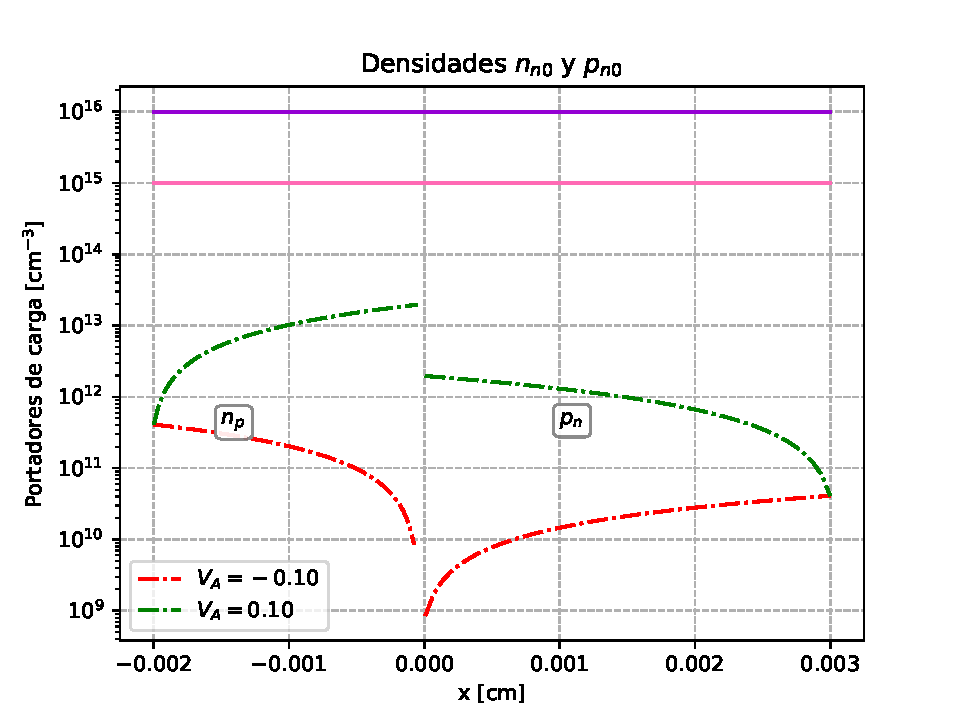
\includegraphics[width=0.7\linewidth]{Ejercicios/Ch_03/03_09_portadores.pdf}
   \end{center}
    \item Calculamos la corriente total y las componentes en la siguiente imagen (usando las ecuaciones del diodo estrecho):
    \begin{equation}
        I_{P}(x_n) = q A \frac{D_P}{L_P} p_{n0} \coth \parentesis{\frac{x_{1n}-x_n}{L_N}}  \parentesis{e^{qV_A/kT}-1} 
    \end{equation}
    \begin{equation}
        I_{N}(x_p) = q A \frac{D_N}{L_N} n_{p0} \coth \parentesis{\frac{x_{1p}-x_p}{L_N}}  \parentesis{e^{qV_A/kT}-1}
    \end{equation}
    Tal que los resultados numéricos son: 
    \begin{equation}
        V_a=\SI{1.0e-01}{[V]} \quad 
        I_N(x_p)=\SI{1.610e-03}{[A]} \quad 
        I_P(x_n)=\SI{5.346e-05}{[A]}
    \end{equation}
    \begin{equation}
        I_T = \SI{1.663e-03}{[A]}
    \end{equation}
    \begin{equation}        
        V_a=\SI{-1.0e-01}{[V]} \quad 
        I_N(x_p)=\SI{-3.409e-05}{[A]} \quad 
        I_P(x_n)=\SI{-1.118e-06}{[A]}
    \end{equation}
    \begin{equation}
        I_T = \SI{-3.52e-05}{[A]}
    \end{equation}
    \begin{center}
     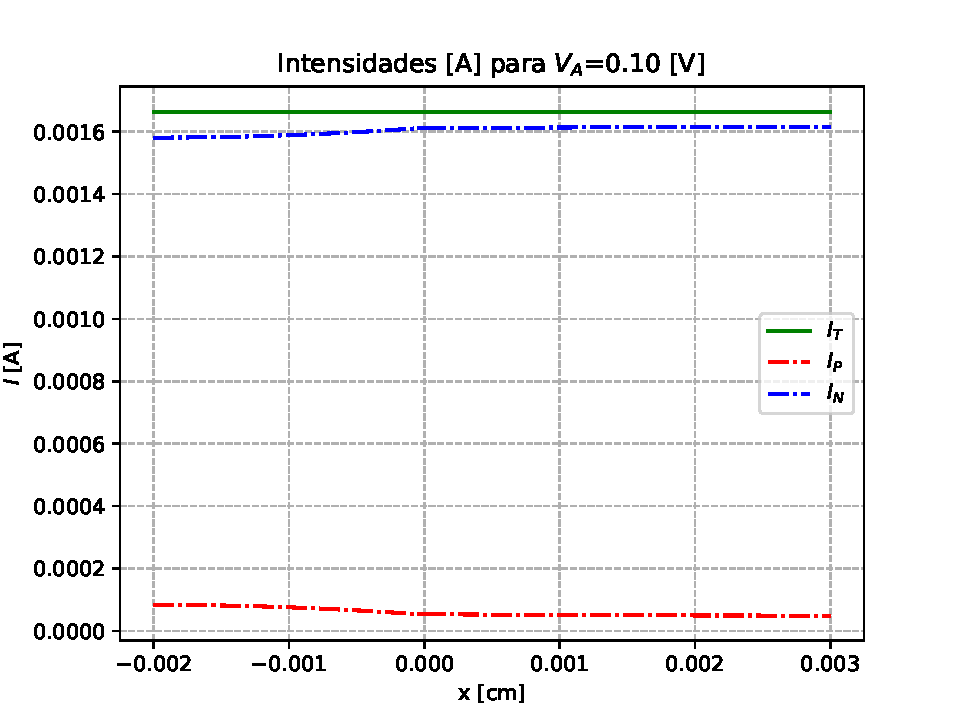
\includegraphics[width=0.7\linewidth]{Ejercicios/Ch_03/03_10_corrientes.pdf}
    \end{center}
    \begin{center}
     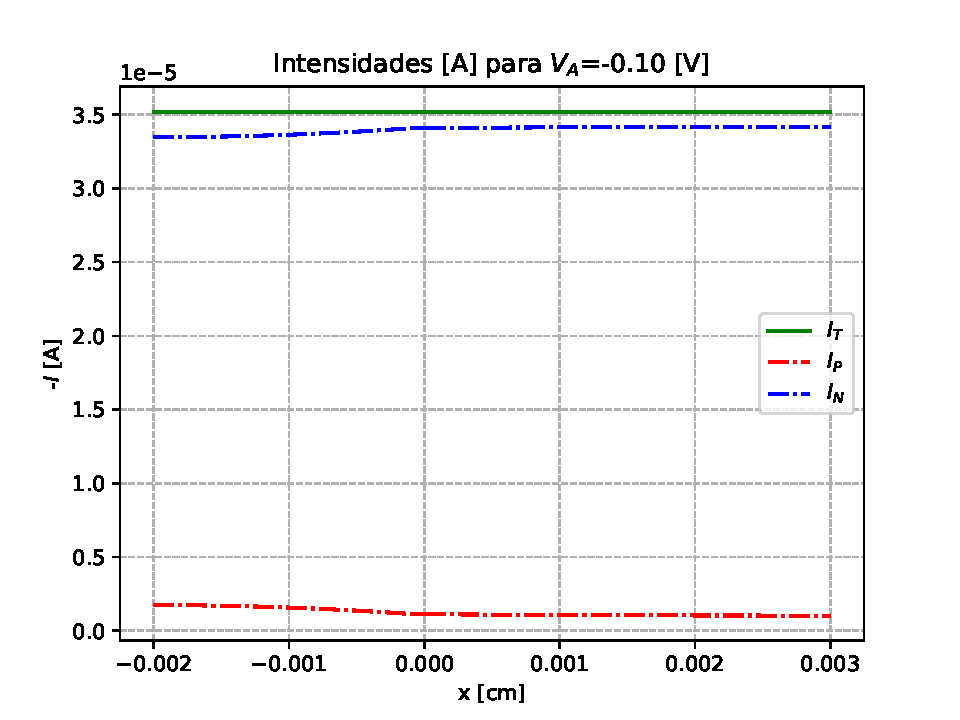
\includegraphics[width=0.7\linewidth]{Ejercicios/Ch_03/03_11_corrientes.pdf}
    \end{center}
    
\end{enumerate}



%---------------------------
% Ejercicio 3
%---------------------------

\begin{Enunciado}
	\subsection*{Ejercicio 3}
	%\addcontentsline{toc}{subsection}{\textit{Ejercicio 3}}
    
	\lipsum[1].
\end{Enunciado}

\vspace*{1em}

\lipsum[1].

%---------------------------
% Ejercicio 4
%---------------------------

\begin{Enunciado}
	\subsection*{Ejercicio 4}
	%\addcontentsline{toc}{subsection}{\textit{Ejercicio 4}}
    
	\lipsum[1].
\end{Enunciado}

\vspace*{1em}

\lipsum[1].

\vspace*{2em}

%%%%%%%%%%%%%%%%%%%%%%%%%%%%%%%%%%%%%%%%%%%%%%%%%%%%%%%%%%%%%%%%%%%%%%%
%%%%%%%%%%%%%%%%%%%%%%%%% EJERCICIOS 5 %%%%%%%%%%%%%%%%%%%%%%%%%%%%%%%%
%%%%%%%%%%%%%%%%%%%%%%%%%%%%%%%%%%%%%%%%%%%%%%%%%%%%%%%%%%%%%%%%%%%%%%%


\subsection*{Ejercicio 5} 

\begin{Enunciado}
    
En una unión PN de silicio que en la zona de vaciamiento tiene $J_n = 25$ mA/cm$^2$ y 
$J_p = 7$ mA/cm$^2$ a $V_A = 0.5$ V. ($D_n = 21$ cm$^2$/s, $D_p = 10$ cm$^2$/s, 
$\tau_{p0} = \tau_{n0} = 5 \times 10^{-7}$ s), calcula y representa:

\begin{itemize}
    \item El diagrama de bandas de energía para esa polarización.
    \item La concentración de portadores de cada tipo en todo el dispositivo.
\end{itemize}


\end{Enunciado}
El ejercicio 5:

\begin{itemize}
    \item Nos dan los valores de $J_N$ y $J_P$ en la región de vaciamiento, cque vienen dadas por
    \begin{equation*}
        J_N = q \frac{D_N}{L_N} n_{p0} \parentesis{e^{qV_A/kT}-1}      \tquad    J_P = q \frac{D_P}{L_P} p_{n0} \parentesis{e^{qV_A/kT}-1}
    \end{equation*}
    y como conocemos $D_N,D_P,L_N,L_P$ y $V_A$, podemos despejar:
    \begin{equation}
        L_N = \sqrt{D_N \tau_n} = 0.32 \ \unit{cm} \qquad L_P = \sqrt{D_P \tau_p } = 0.22 \ \unit{cm}
    \end{equation}
    \begin{equation*}
        n_{p0} = \frac{J_N}{q} \frac{L_N}{D_N} \frac{1}{\parentesis{e^{qV_A/kT}-1} } = 9.6\cdot 10^5 \cm^{-3} \qquad p_{n0} = \frac{J_P}{q} \frac{L_P}{D_P} \frac{1}{\parentesis{e^{qV_A/kT}-1} }     = 3.9\cdot 10^5 \cm^{-3} 
    \end{equation*}
    Que como conocemos $n_i$ a la temperatura de 300 K:
    
    \begin{equation*}
        n_i = 10^{10} \ (\cm^{-3})
    \end{equation*}
    significa que podemos conocer $N_A$ y $N_D$, tal que:

    \begin{equation*}
        N_A = \frac{n_i^2}{n_{p0}} = \SI{1.042e+15}{cm^{-3}} \tquad N_D = \frac{n_i^2}{p_{n0}} = \SI{2.569e+15}{cm^{-3}} 
    \end{equation*}
    y ahora podemos usar las siguientes ecuaciones para calcular los valores de $E_c,E_i$ y $E_v$ respecto $E_F$: 

    \begin{equation*}
        E_i |_P =  kT \ln \parentesis{\frac{N_A}{n_i}} \quad E_c |_P = \frac{E_g}{2} + E_i + \frac{3}{4}kT \frac{m_n^*}{m_p^*} \quad E_v|_P = E_c|_P - E_g
    \end{equation*}
    Tal que:

    \begin{equation*}
        E_i|_N = E_i|_P - V_{bi} +V_a  \quad E_i|_N = E_i|_P - V_{bi} + V_a \quad E_i|_N = E_i|_P - V_{bi} +V_a
    \end{equation*}
    donde 
    \begin{equation*}
        \Vbi = \frac{kT}{q} \ln \parentesis{\frac{N_A N_D}{n_i^2}}  = 0.621 \ \unit{V}
    \end{equation*}       
    y así $\Vbi^\text{eff} = \Vbi - V_A = 0.121$ V. Falta escribir:
    
    \begin{equation}
        x_n = 1.32 \cdot 10^{-5} \ \cm \tquad x_p = 3.26 \cdot 10^{-5} \ \cm
    \end{equation}    
    El diagrama de bandas con polarización $V_A=0.5$ V

    \begin{center} 
        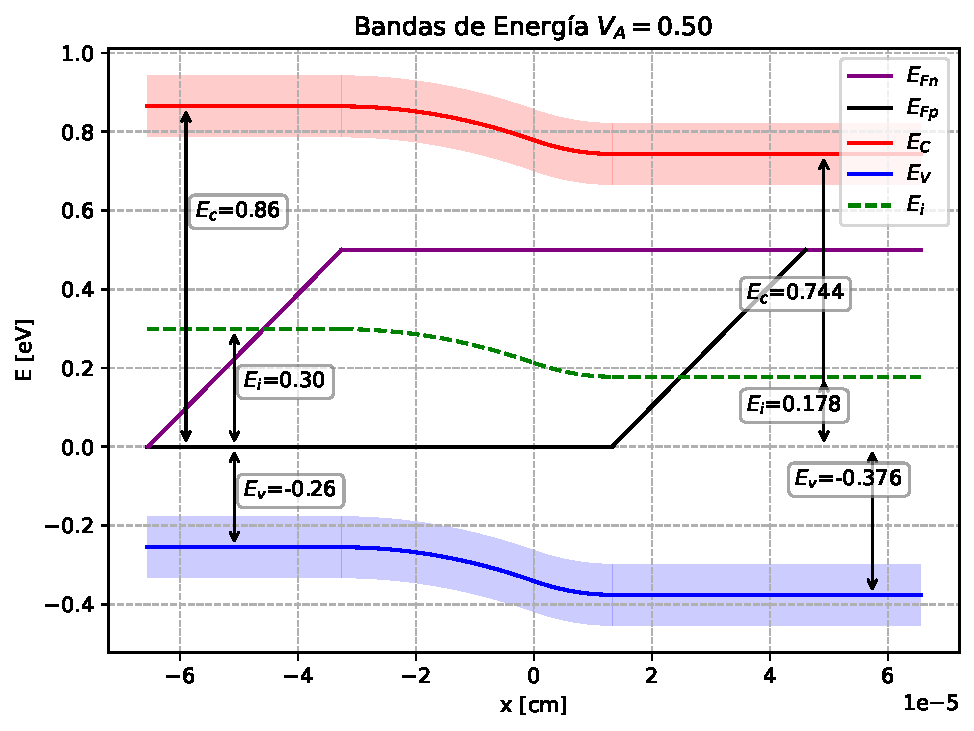
\includegraphics[width=0.7\linewidth]{Ejercicios/Ch_03/03_05_01.pdf}
    \end{center}


    \item La concentración de portadores en todo el dispositvo se calcula usando las siguientes ecuaciones, suponiendo un diodo ideal infinito: 
    
    \begin{equation*}
        n_{p} = n_{p0} + n_{p0} \parentesis{e^{qV_A/kT}-1} e^{(x+x_p)/kT}  \tquad  n_n = N_D
    \end{equation*}
    \begin{equation*}
        p_{p} = N_A \tquad p_{n} (x) = p_{n0} \parentesis{e^{qV_A/kT}-1} e^{-(x-x_n)/kT}  
    \end{equation*}
    En la región de vaciamiento suponemos que $n$ y $p$ son rectas que conectan los valores límites. La gráfica en el caso de polarización $V_A=0.5$ V: 
    \begin{figure}[h!] \centering
        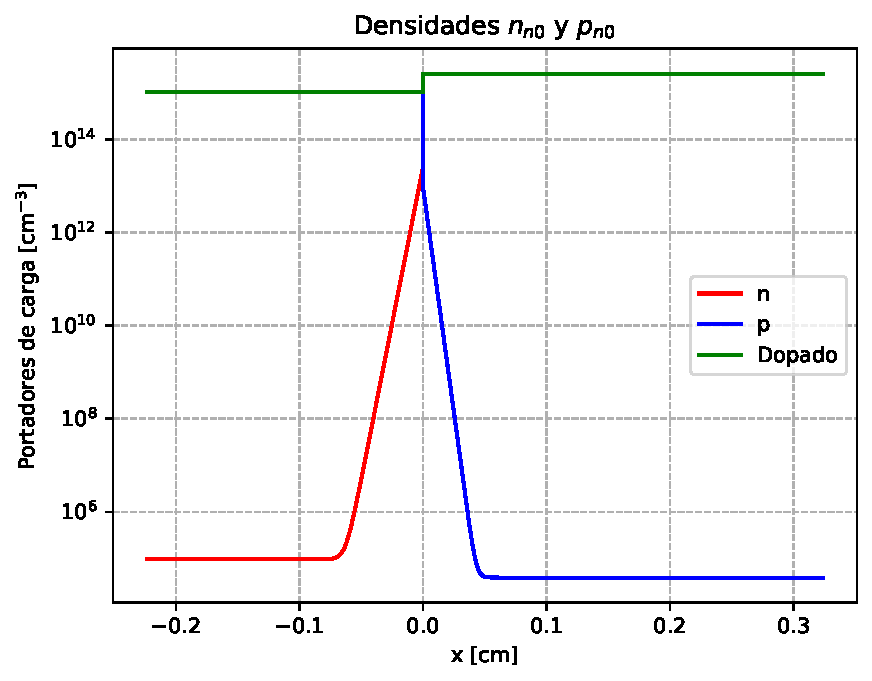
\includegraphics[width=0.7\linewidth]{Ejercicios/Ch_03/03_05_02.pdf}
    \end{figure}

\end{itemize}




%%%%%%%%%%%%%%%%%%%%%%%%%%%%%%%%%%%%%%%%%%%%%%%%%%%%%%%%%%%%%%%%%%%%%%%
%%%%%%%%%%%%%%%%%%%%%%%%% EJERCICIOS 6 %%%%%%%%%%%%%%%%%%%%%%%%%%%%%%%%
%%%%%%%%%%%%%%%%%%%%%%%%%%%%%%%%%%%%%%%%%%%%%%%%%%%%%%%%%%%%%%%%%%%%%%%

\subsection*{Ejercicio 6} 
\begin{Enunciado}
    

Si tenemos una unión NP polarizada en directa, $V_A = 0.2$ V:

\begin{itemize}
    \item Representar el diagrama de bandas de energía.
    \item Obtener el valor de la densidad de corriente de cada tipo de portador y representarla en todo el dispositivo.
\end{itemize}

Datos: $A = 2$ mm$^2$, $T = 300$ K, $E_{gap} = 1.42$ eV, $N_D = N_A = 10^{14}$ cm$^{-3}$, $\mu_n = 9000$ cm$^2$/Vs, $\mu_p = 450$ cm$^2$/Vs, $\tau_p = 20$ ns, $\tau_n = 10$ ns, $\varepsilon = 1.4337 \times 10^{-12}$ F/cm, $m_e/m_0 = 0.4$, $m_h/m_0 = 0.3$.


\end{Enunciado}

Hay que recordar que una unión np es igual que la union pn pero donde $x\rightarrow -x$
\begin{itemize}
    \item Usamos las siguientes ecuaciones para calcular los valores de $E_c,E_i$ y $E_v$ respecto $E_F$: 
    
    \begin{equation*}
        E_i|_P =  k T \ln \parentesis{\frac{N_A}{n_i}} \qquad E_c|_P = \frac{E_g}{2} + E_i + \frac{3}{4} kT \ln \parentesis{\frac{m_n^*}{m_p^*}} \qquad E_v |_P = E_c - E_g
    \end{equation*}
    \begin{equation*}
        E_i|_N = E_i - \Vbi^\text{eff}  \qquad E_c|_N = E_c|_N - \Vbi^\text{eff} E_v |_N = E_v|_N - \Vbi^\text{eff} 
    \end{equation*}
    donde hemos usado que ($K_S=16.2$)

    \begin{equation*}
        n_i = 2 \parentesis{\frac{kT (m_n^* m_p^* )^{1/2}}{2\pi \hbar^2}}^{3/2} e^{-\frac{E_g}{2kT}} 
    \qquad \Vbi^{\text{eff}} = \Vbi - V_a \quad \Vbi = \frac{kT}{q} \ln \parentesis{\frac{N_AN_D}{n_i^2}}
    \end{equation*}
    \begin{equation}
        n_i=\SI{6.046e+6}{cm^{-3}} \quad \Vbi = 0.859 
    \end{equation}
    \begin{equation}
        D_N = 232.67 \ \cm^2/s \quad D_P =  11.63 \ \cm^2/s \quad L_N = 15.21 \ \mu \unit{m} \quad L_P = 4.82 \  \mu \unit{m}
    \end{equation}
    \begin{equation}
        x_n = \SI{2.429e-4}{cm} \tquad 
        x_p = \SI{2.429e-4}{cm}  
    \end{equation}
    Así pues, el diagrama de bandas con polarización $V_A=0.5$ V: 

    \begin{center} 
        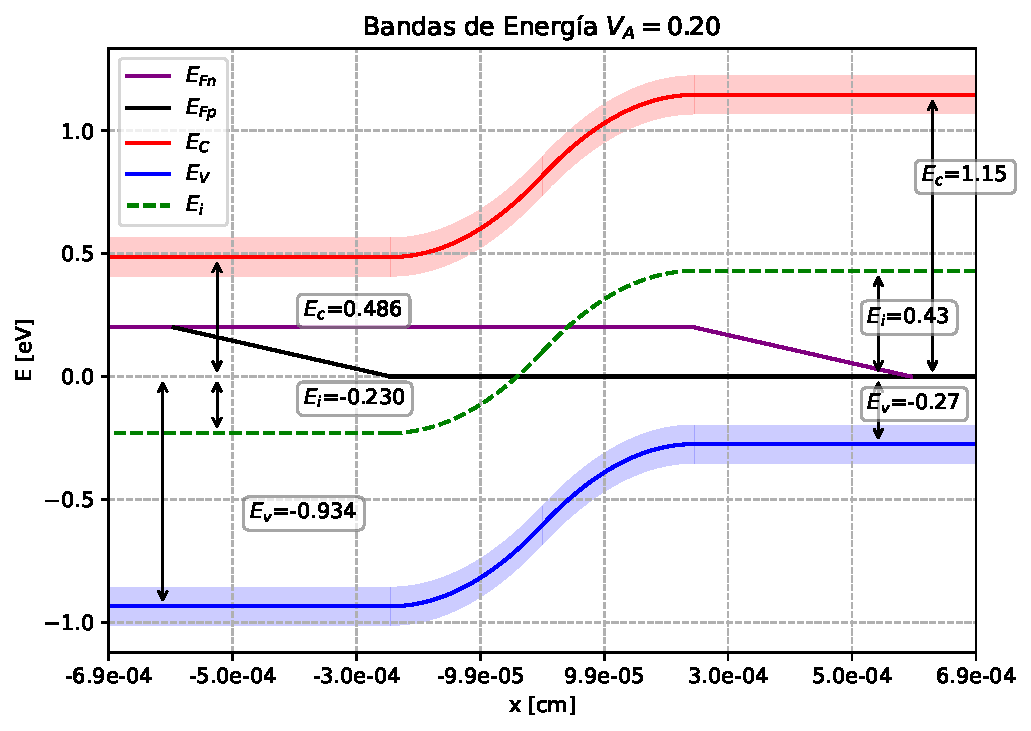
\includegraphics[width=0.6\linewidth]{Ejercicios/Ch_03/03_06_01.pdf}
    \end{center}
    

    \item Los valores de las intensidades en todo el dispositvo se calcula usando las siguientes ecuaciones: 
    
    \begin{equation*}
        \text{Zona P:} \quad 
        I_N(x) = -qA\frac{D_N}{L_N} \frac{n_i^2}{N_A}  \parentesis{e^{qV_A/kT}-1} e^{(x+x_p)/L_N} \quad I_P(x) = I_T - I_N (x)
    \end{equation*}
    \begin{equation*}
        \text{Zona N:} \quad 
        I_P(x) = - qA\frac{D_P}{L_P} \frac{n_i^2}{N_D}  \parentesis{e^{qV_A/kT}-1} e^{(-x+x_n)/L_P} \quad I_N(x) = I_T - I_P (x)
    \end{equation*}
    tal que:

    \begin{equation*}
        I_T = -qA\parentesis{\frac{D_N}{L_N} \frac{n_i^2}{N_A}+\frac{D_P}{L_P} \frac{n_i^2}{N_D}}  \parentesis{e^{q V_A/kT}-1}
    \end{equation*}
    Al ser NP tenemos que el signo cambia, al ser polarización directa la corriente va de P a N (recordemos que en polarización directa predomina la corriente de difusión, que tiene la dirección P$\rightarrow$M, que en este caso significa corriente negativa). Y los valores numéricos:

    \begin{equation}
        I_P (x_n) = \SI{-6.467e-14}{C/s} \qquad 
        I_N (x_p) = \SI{-4.737e-13}{C/s} \qquad
        I_T = \SI{4.737e-13}{C/s}
    \end{equation}

    Obteniendo la siguiente gráfica para $V_A=0.2$ V: 


    \begin{center} 
        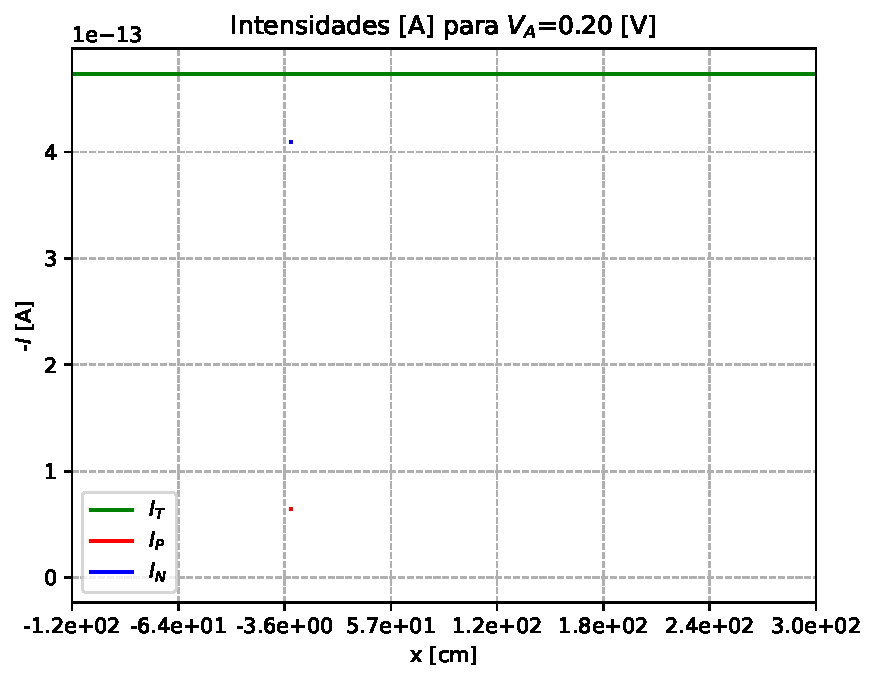
\includegraphics[width=0.6\linewidth]{Ejercicios/Ch_03/03_06_02.pdf}
    \end{center}
    
\end{itemize}



%%%%%%%%%%%%%%%%%%%%%%%%%%%%%%%%%%%%%%%%%%%%%%%%%%%%%%%%%%%%%%%%%%%%%%%
%%%%%%%%%%%%%%%%%%%%%%%%% EJERCICIOS 7 %%%%%%%%%%%%%%%%%%%%%%%%%%%%%%%%
%%%%%%%%%%%%%%%%%%%%%%%%%%%%%%%%%%%%%%%%%%%%%%%%%%%%%%%%%%%%%%%%%%%%%%%

\begin{Enunciado}
\subsection*{Ejercicio 7} 

Si partimos de una unión PN de silicio, con el lado P dopado de forma gradual con 
$a = 10^{19}$ cm$^{-4}$ y el lado $N_D = 3.0 \times 10^{14}$ cm$^{-3}$ constante. 
Bajo condición de equilibrio, si el ancho de la zona de vaciamiento de la zona P es 
de 0.8 micras, calcular y representar el ancho total de la zona de vaciamiento, 
el campo eléctrico y el potencial de contacto.

\end{Enunciado}

Si suponemos que la densidad de carga es:

\begin{equation*}
    \rho (x) = \left\lbrace \begin{array}{ll}
        -q a x & -x_p < x < 0  \\ 
        q N_D & 0 < x < x_n  
    \end{array} \right.
\end{equation*}
El campo eléctrico viene dado por:

\begin{equation*}
    \Ecal (x) =  \left\lbrace \begin{array}{ll}
        \frac{qa}{2K_S\varepsilon_0} \ccorchetes{x^2 - x_p^2} & -x_p < x < 0  \\ 
        \frac{qN_D}{K_S\varepsilon_0} \ccorchetes{x- x_n} & 0 < x < x_n  
    \end{array} \right. 
\end{equation*}
\begin{equation*}
    \Ecal_{\min} = -49500 \ \unit{V/cm} 
\end{equation*}
Exigimos que el campo en $x=0$ debe ser igual en ambos lados:

\begin{equation}
    \frac{qN_D}{K_S \epsilon_0} x_n = \frac{qa}{2K_S\epsilon_0} x_p^2 \rightarrow x_n = \frac{a x_p^2}{2 N_D} = 1.06 \ \unit{\mu m} \quad W = 1.86 \ \unit{\mu m}
\end{equation}


donde hemos exigido que $\Ecal(x_n)=0$ y $\Ecal(-x_p)=0$. El potencial de contacto:
\begin{equation*}
    V (x) =  \left\lbrace \begin{array}{ll}
        \frac{qa}{6K_S\varepsilon_0} \ccorchetes{x^3 - 3x_p^2 x + A} & -x_p < x < 0  \\ 
        \frac{qN_D}{2K_S\varepsilon_0} \ccorchetes{x^2 - 2x_n x + B} & 0 < x < x_n  
    \end{array} \right.
\end{equation*} 
Para que $V(-x_p)=0$ tendría que verificarse $A=2x_p^3$. También se tiene que verficiar que $V(0)|_{-}=V(0)|_{+}$, y por tanto: 

\begin{equation*}
    \frac{qa A}{6K_S\varepsilon_0} = \frac{qN_D B}{2K_S\varepsilon_0} \rightarrow B = \frac{2 a x_p^3}{3 N_D}
\end{equation*}
El valor del voltaje final: 
\begin{equation*}
    V (x) =  \left\lbrace \begin{array}{ll}
        \frac{qa}{6K_S\varepsilon_0} \ccorchetes{-x^3 + 3x_p^2 x + 2x_p^3} & -x_p < x < 0  \\ 
        \frac{qN_D}{2K_S\varepsilon_0} \ccorchetes{-x^2 + 2x_n x + \frac{2 a x_p^3}{3 N_D}} & 0 < x < x_n  
    \end{array} \right.
\end{equation*}
Sería interesante definir ahora el valor de $\Vbi$ y vr si coincide con $V(x_n)$. Así tenemos que:

\begin{equation}
    \Vbi = \frac{qN_D}{2K_S\epsilon_0} \ccorchetes{-x_n+\frac{2ax_p^3}{3N_D}} = 0.525 \ \unit{V}
\end{equation}
Tenemos pues que: 
\begin{equation}
    \Vbi^* = \frac{kT}{q} \ln \parentesis{\frac{x_p a N_D}{n_i^2}} = 0.558 \ \unit{V}
\end{equation}



%---------------------------
% Ejercicio 7
%---------------------------
\begin{Enunciado}
	\subsection*{Ejercicio 8}
	%\addcontentsline{toc}{subsection}{\textit{Ejercicio 7}}
	\lipsum[1].
\end{Enunciado}
\vspace*{1em}
\lipsum[1].
\vspace*{2em}

%---------------------------
% Ejercicio 8
%---------------------------
\begin{Enunciado}
	\subsection*{Ejercicio 9}
	%\addcontentsline{toc}{subsection}{\textit{Ejercicio 8}}
    
	\lipsum[1].
\end{Enunciado}
\vspace*{1em}
\lipsum[1].
\vspace*{2em}
%---------------------------
% Ejercicio 9
%---------------------------
\begin{Enunciado}
	\subsection*{Ejercicio 10}
	%\addcontentsline{toc}{subsection}{\textit{Ejercicio 9}}
    
	\lipsum[1].
\end{Enunciado}
\vspace*{1em}
\lipsum[1].

\chapter{Estructura nuclear} \label{Ch:04}

\section{Introducción a la estructura nuclear}

Un núcleo atómico es un objeto constituido por muchos cuerpos (el Uranio tiene hasta 238 nucleones). Describir las propiedades nucleares a partir de la interacción básica entre esos cuerpos es una tarea formidable y fuera de nuestro alcanceen la actualidad por varias razones. En primer lugar la interacción entre dos nucleones no está del entendida desde el punto de vista teórico-conceptual\footnote{La Cromodinámica Cuántica (QCD) aunque ha superado pruebas experimentales, no permite hacer cálculos predictivos, y mucho menos deducir a partir de ella las características de interacción fuerte entre hadrones.}, y en segundo lugar, aunque dispusiéramos de una teoría completa que describiese la interacción en todos sus detalles no podríamos manejar operativamente el difícil problema de la interacción entre muchos cuerpos. Esto nos lleva de modo natural a intentar a describir la estructura nuclear y el espectro de excitaciones a partir de de modelos muy simplificados, esto es, modelos construidos a partir de algunas de las propiedades de los núcleos en lugar de las funciones de onda detalladas de cada nucleón. Se utiliza un planteamiento similar en la termodinámica, donde variables colectivas como la presión y la temperatura de un gas sustituyen a las variables cinemáticas de cada uno de sus átomos. A grandes rasgos, podemos clasificar los modelos de estructura nuclear en dos categorías:

\begin{itemize}
    \item \textbf{Modelos de fuerte correlación:} las propiedades nucleares sobre las que se construyen este tipo de modelos se explican como originadas a partir del comportamiento colectivo de los nucleones. Un ejemplo podrían ser los movimientos rotacionales y vibratorios nucleares, que dan lugar a espectros característicos de energía cuantizada. Es obvio que un movimiento rotatorio es un fenómeno creado por un comportamiento colectivo o correlacionado de los nucleones.
    \item \textbf{Modelo de casi nula corrección:} las características nucleares propias de estos modelos se suponen originadas por el comportamiento individual de cada nucleón.
\end{itemize}
Ninguno de los dos tipos de modelo en su versión extrema pueden explicar todas las propiedades nucleares. Los modelos más realistas tratan con una mezcla de propiedades colectivas e individuales de los nucleones. Un modelo basado exclusivamente en propiedades colectivas será insuficiente para explicar parte de las propiedades nucleares, y es necesario acudir a una cierta mezcla de propiedades colectivas e individuales para conseguir modelos nucleares con un rango de aplicación más interesante.

\section{El modelo de la gota líquida}

El modelo de la gota líquida lo hemos aplicado ya en un capítulo anterior para obtener la fórmula semiempírica de masas o fórmula de Weizsäcker, que nos permite calcular las masas y las energías de ligaduras de los núcleos. Una gota de líquido en ausencia de campos gravitatorios (o cualquier otro tipo de campo) adquiere una forma que minimiza la energía positiva de tensión superficial. Esta forma es la forma de la esfera. Una gota de líquido es esencialmente incompresible (su densidad es constante), y por lo tanto su radio será $R\sim n^{1/3}$, donde $n$ es el número de moléculas de la gota. Consideremos que la gota tiene una energía de ligadura\footnote{Las moléculas de la superficie estarán menos ligados que las interiores, pero este efecto se introduce como una corrección en términos de la tensión superficial.}  que podemos denotar por $a$ La energía de ligadura se debe a la interacción de la molécula con sus moléculas vecinas. Estas fuerzas de interacción se anulan a distancias grandes y se hacen repulsivas a distancias cortas comparadas con la distancia intermolecular típica\footnote{La interacción fuerte entre nucleones tiene características similares en cierto sentido, como veremos más adelante.}. Si tomamos como cero la energía la situación en la cual todas las moléculas de la gota están infinitamente separadas, podemos expresar la energía de ligadura de la gota (tomada positiva) de la siguiente manera:

\begin{equation}
    B=an - 4 \pi R^2 T = an-\beta n^{2/3} \quad (R^2 \sim n^{2/3})
\end{equation}
donde $T$ es la energía de tensión superficial del líquido. Si la gota tuviese una carga eléctrica $Q$ uniformemente distribuida en todo su volumen debemos añadir un término correspondiente a la energía potencial coulombiana:

\begin{equation}
    B = an - \beta n^{2/3} - \frac{\gamma Q^2}{n^{1/3}}
\end{equation}
donde $\gamma$ contiene todas las contantes de la energía coulombiana excepto la dependencia con $Q$ y $n$. 

Para obtener la fórmula de Weizsäcker, o fórmula semiempírica de masas, aplicamos estas ideas y algunas otras hipótesis de trabajo que recapitulamos aquí:

\begin{itemize}
    \item Suponemos un núcleo esférico.
    \item Los nucleones dentro del núcleo se comportan de modo análogo a moléculas en una gota líquida, es decir, fuerzas atractivas de corto alcance los mantienen unidos y fuerzas repulsivas, de todavía más corto alcance, los mantienen alejados unos de otros.
    \item La densidad nuclear es constante. 
    \item Existe una tendencia a mantener un número de protones muy parecidos al número de neutrones en un núcleo.
    \item Existe una \textit{fuerza de apareamiento} que favorece la existencia de núcleos con $Z$ par y $N$ par.
\end{itemize}

\section{El modelo de Gas de Fermi}

Alrededor de 1948, se comenzó a considera en serio la evidencia acumulada sobre la existencia de ciertos \textbf{números mágicos} para los valores de $Z$ y $N$. La energía de separación de dos protones para secuencias de isótonos ($N$ constante) graficada como desviaciones de la predicción de la fórmula semiempírica de masas, mostraba unos picos acusados par $Z=8,20,28,50,83$; mientras que la energía de separación de dos neutrones para secuencias de isótopos, también graficada como desviaciones de la predicción de la fórmula semiempírica de masas muestra picos para $N=8,20,28,50,82,126$. La similitud de estas gráficas con la de algunas propiedades atómicas, como la energía de ionización es sorprendente. Recordemos que estas propiedades atómicas tienen su origen en la formación de \textit{capas cerradas} de electrones moviéndose \textit{independientemente} en un potencial efectivo atómico. Sin resistencia a pesar que los nucleones se pudiera mover independientemente en el núcleo sin interaccionar (o apenas interaccionando) los unos con los otros, sobre todo debido al éxito del modelo nuclear de la gota líquida en la explicación aproximada de las masas de los núcleos.

Los datos experimentales indican que los nucleones parecen comportarse de dos maneras contradictorias: por un lado, como un grupo de partículas fuertemente interaccionantes en un especie de estado condensado con características similares a las de un líquido, y por otro como un sistema de partículas que apenas interaccionan entre sí, con características propias de un gas. A la hora de comprender estas características aparentemente contradictorias resultas útil introducir la abstracción de \textbf{materia nuclear} sin repulsión coulombiana, y tan grande que pudiésemos despreciar los efectos de superficie. Weisskopf fue el primero en tratar de explicar las propiedades de la materia nuclear por medio del modelo del \textbf{gas de Fermi}, en completo analogía con el modelo que se usa para explicar las propiedades de conducción eléctrica de los metales considerando un \textit{gas de electrones libres}.

Se supone que cada nucleón se mueve libremente en un pozo de potencial neto atractivo creado por todos los demás nucleones. Este potencial neto tiene una profundidad constante en el núcleo puesto que la distribución de nucleones es constante en esta región, y se aproxima a cero rápidamente en una distancia que coincide con el rango del alcance de la fuerza nuclear fuerte. Cuando el núcleo se encuentra en su estado fundamental todos los nucleones ocupan los niveles más bajos de energía del pozo de potencial y el llenado de niveles se realiza de acuerdo con el principio de exclusión de Pauli. Esto significa que no es posible que exista transferencia de energía (interacción) entre dos nucleones, porque ello supondría desplazarlos de sus niveles energéticos y estamos asumiendo que todos los niveles están ya ocupados\footnote{Un intercambio de niveles entre dos nucleones no representa ninguna interacción, porque los nucleones son indistinguibles.}. Únicamente sería posible que uno de los nucleones saltase a uno de los niveles de valencia desocupados, pero eso requiere más energía de la habitualmente disponible en el movimiento de los nucleones dentro de un núcleo en su estado fundamental.


Podemos entonces suponer de forma aproximada que los nucleones se encuentran en un pozo esférico de potencial cuyo perfil puede verse esqumáticamente en la figura \ref{Fig:04-01}. Para un núcleo de $A \sim 100$ el radio del pozo de potencial sería $R_c \sim$5.6 fm, lo cual es suficientemente para evitar que los efectos de superficiie sean los dominantes. En este esquema simplificado, el pozo de potencial para los protones no es el mismo que para los neutrones. El de los protones es un poco menos profundo debido a la repulsión coulombiana que ellos sienten y los neutrones no. Además, para los protones tenemos una barrera coulombiana que alza el extremo superior del pozo unas decenas de MeV (nótese la línea roja, que es la región del potencial de protones).

\begin{figure}[h!] \centering
	\begin{pspicture}(-1,-5)(6,3)
		\psline[arrowscale=2,linewidth=1pt]{->}(0,-4)(0,3)
		\psline[linewidth=1pt](0,-4)(2,-4)
		\psline[linewidth=1pt](2,-4)(2,0)
		\psline[arrowscale=2,linewidth=1pt]{->}(2,0)(6,0)
		\psline[linewidth=0.9pt](0,-0.4)(2,-0.4)
		
		\psline[linewidth=0.9pt,linearc=2,linecolor=red,linestyle=dashed](0,-3)(1,-3.5)(2,-3.5)
		\psline[linewidth=0.9pt,linearc=2,linecolor=red,linestyle=dashed](2,1)(3.5,0.1)(5,0.1)
		\psline[linewidth=0.9pt,linearc=2,linecolor=red,linestyle=dashed](2,0)(2,1)
		\psline[linewidth=0.9pt,linearc=2,linecolor=red,linestyle=dashed](0,-0.6)(2,-0.6)
		
		\rput(2.5,1.5){\textcolor{red}{{\small Pozo de protones}}}
		\rput(1.0,-4.5){{\small Pozo de neutrones}}
		
		\rput(-0.4,2.0){V(r)}
		\rput(5.0,-0.5){r}
		
		\psline[linewidth=0.75pt,arrowscale=1]{<->}(0,-1.2)(2,-1.2)
		\rput(1.0,-1){$R_c$}
		
		\psline[linewidth=0.75pt,arrowscale=1]{<->}(2.2,-4)(2.2,-0.4)
		\rput(4.0,-2){{\footnotesize  $E_f \sim 33 \ \unit{\MeV}$ (neutrones)}}
		
		\psline[linewidth=0.55pt,arrowscale=1]{<->}(2.5,-0.4)(2.5,-0.0)
		\rput(3.2,-0.2){{\footnotesize  $\sim 8 \ \unit{\MeV}$}}
		
		
	\end{pspicture}
	\caption{Aproximación del potencial por un pozo.}
	\label{Fig:04-01}
\end{figure}

Los nucleones llenarían sus respectivos niveles energéticos en estos pozos de potencial de acuerdo con el principio de exclusión de Pauli hasta una energía cinética máxima conocida como \textbf{energía de Fermi}, $E_F$. Esta energía se puede estimar suponiendo un núcleo de volumen $4\pi R^3/3$ y número de nucleones constituyentes conocido. A la energía de Fermi le corresponde un momento de Fermi dado por $E_F=p_F^2 / 2m$, y un volumen en el espacio de momentos $V_p=4\pi p_F^2/3$, de tal manera que el volumen disponible en el espacio de fases sería:

\begin{equation}
	V_{\text{ef}} = \parentesis{\frac{4}{3}\pi}^2 (r_0 p_F)^3 A 
\end{equation}
donde $r_0 \sim 1.2 $ fermis y $A$ es el número másico. Ahora bien, de acuerdo con el principio de Heisenberg el mínimo volumen en el espacio de fases que se puede asociar a un estado físico de cualquier sistema es $V_{\text{ef-min}}\sim h^3$ (siendo $h$ la constante de Planck), por lo tanto el número de nucleones que se puede acomodar en el volumen del espacio de fases hasta el nivel de Fermi, teniendo en cuenta el factor 2 debido a fermiones de espín 1/2 será:

\begin{equation}
	n_F = \frac{2}{\hbar^3}V_{\text{ef}} = \frac{4}{9\pi} \parentesis{\frac{r_0 p_F}{\hbar}}^3 A
\end{equation}
Si ahora tomamos en consideración la situación habitual en que $Z=N=A/2$ y por lo tanto $n_F=A/2$ entonces conseguimos la siguiente estimación para el momento y la energía de Fermi:

\begin{equation}
	p_F = \frac{\hbar}{r_0} \parentesis{\frac{9\pi}{8}}^{1/3} \quad E_F = \frac{p_F^2}{2m} = \frac{1}{2m} \parentesis{\frac{\hbar}{r_0}}^2 \parentesis{\frac{9\pi}{8}}^{2/3} \sim 33\ \unit{\MeV}
\end{equation}
Concluimos por tanto que para los neutrones podemos tomar aproximadamente $E_F\sim 33 \ \unit{\MeV}$ e independiente de $A$. Por otro lado, el nivel de energía de Fermi debe coincidir con el nivel que ocupe el nucleón menos ligado, que está a una distancia del nivel de energía cero (situación en la que el nucleón no está ligado al núcleo) igual a la energía de separación. La profundidad del pozo de neutrones será igual entonces a la suma de la energía de Fermi ($\sim 33 \ \unit{\MeV}$) más la energía de separación ($\sim 8 \ \unit{\MeV}$), lo cual nos da unos 40 MeV. Es interesante reflexionar sobre el hecho de que únicamente a partir del tamaño nuclear y del principio de incertidumbre podamos estimar la profundidad del pozo de potencial nuclear. 


A pesar de que las profundidades en los pozos de protones y neutrones son distintas, lo que provoca por ejemplo que los núcleos con $N>Z$ sean mas estables que con $Z>N$, las energías de Fermi deben estar aproximadamente en la misma posición por debajo del valor cero en el pozo de potencial, de lo contrario no habría estabilidad, y la energía de separación del último nucleón sería dependiente de la carga, lo cual estaría en contradicción con las observaciones experimentales.





\section{El modelo de capas}

A semejanza del modelo atómico de capas que tanto éxito a tenido en la física atómica, resulta tentador preguntarse si un modelo similar no tendría éxito también en la física nuclear. Es necesario, sin embargo, tener en cuenta las profundas diferencias entre la física atómica y la nuclear. 

Los electrones se mueven en un potencial externo aproximadamente central: el potencial que crea el núcleo junto con las correcciones oportunas debidas al resto de electrones. De este modo manera surgen natural las capas electrónicas, que se van llenando en orden de energía creciente cumpliendo el principio de exclusión de Pauli. Las capas electrónicas llenas forman una especie de zona interior neutra y los electrones de la capa semillena constituyen los electrones de valencia, que determinan la mayoría de las propiedades químicas del átomo correspondiente. Cuando vamos llenando una capa electrónica las propiedades atómicas como la energía de ionización varían suavemente, pero sufren una súbita discontinuidad cuando la capa queda llena y hemos de pasar a la siguiente. 

En un núcleo no tenemos un agente externo que cree el potencial en el que se mueven los nucleones, son ellos mismos los que configuran el potencial efectivo nuclear. Otra compilación o diferencia adicional es que, en principio, parecería que los nucleones debieran tener una probabilidad no despreciable de colisionar los unos con los otros, mientras que eso no sucede con los electrones atómicos. No resulta evidente que podamos considerar a cada nucleón moviéndose independientemente de los demás en un potencial nuclear efectivo, pero ya hemos visto que el principio de exclusión de Pauli garantiza que, esencialmente, los nucleones se mueven libremente dentro del núcleo. 

La hipótesis principal del modelo de capas es suponer que los nucleones se mueven en el núcleo casi independientemente los unos de los otros a pesar de la interacción fuerte. Este movimiento libre significa, en última instancia, que el recorrido libre medio de un nucleón en materia nuclear es grande comparado con las dimensiones del núcleo. En el modelo de capas la interacción nucleón con sus compañeros se reduce a la interacción con un \textbf{campo autoconsciente} (\textit{self-consistent field}) creado por ellos. Generalmente se supone que este campo autoconsciente es estático y esféricamente simétrico.

Debido al corto alcance de las fuerzas nucleares, el potencial del campo autoconsciente tiene dependencia radial muy similiar a la densidad nuclear, es decir, es casi constante dentro del núcleo y se anula fuera. Por lo tanto, en primera aproximación podríamos considerar que el potencial nuclear constante en el interior del núcleo, tal como se hace en el modelo de gas de Fermi ideal\footnote{El modelo de capas incorpora la hipótesis del modelo de gas de Fermi.}, con lo cual las funciones de onda de los nucleones serían ondas planas. No obstante, la introducción den el modelo de capas de un campo autoconsistente que depende de la distancia al centro del núcleo es una mejora sustancial respecto del modelo de gas de Fermi, y modifica las funciones de onda de los nucleones, dejando de ser ondas planas. 

Existen varias versiones del modelo de capas. La más simple, conocida como \textbf{versión extrema del modelo de capas} (\textit{one-particle shell mode}), se usa para explicar las propiedades de los núcleos con $A$ impar. En esta versión se supone que todos los nucleones están apareados (incluyendo los de una hipotética capa semillena) formando una coraza interior de espín cero, y que las propiedades del núcleo se deben únicamente al estado del nucleón desapareado. Una mejora de este modelo consiste en considerar todos los nucleones de la última capa semillena, no sólo el desapareado. El siguiente paso en la elaboración de un modelo más detallado sería, obviamente, considerar todos los nucleones, tanto en las capas llenas como las semillenas.

\subsection{Evidencia experimental de capas en los núcleos}

Hemos visto que para ciertos valores mágicos de $N$ y $Z$ los núcleos muestran una estabilidad inusual, que se manifiesta, por ejemplo, en una energía de separación de dos nucleones (protones o neutrones) grande. Además cuando $Z$, o $N$, o ambos, coinciden con un número mágico, la energía de ligadura nuclear es mayor que la esperada y algunas otras propiedades nucleares, como el radio, se comportan como si se hubiera completado una capa de estados análoga a las capas electrónicas atómicas. El modelo de capas nuclear considera niveles energéticas de los nucleones en un potencial adecuado. Una capa consiste en un grupo de niveles energéticos cercanos. A continuación se ofrece alguna lista de algunas evidencias experimentales en favor de la existencia de números mágicos:

\begin{itemize}
	\item Existen grandes desviaciones en la energía de ligadura nuclear cerca de los números mágicos. 
	\item La energía de separación protónica (neutrónica) tiene picos cuando $Z$ ($N$) es mágico.
	\item La energía cinética de las partículas $\alpha$ es particularmente alta cuando el núcleo hijo tiene un número mágico de neutrones.
	\item Los elementos con $Z(N)$ mágico tienen más isótopos (isótonos) que sus vecinos.
	\item El primer estado excitado $2^+$ de un núcleo par-par tiene una energía excepcionalmente alta si $z$ y $N$ son mágicos.
	\item El radio nuclear decrece en los núcleos con $N$ mágico.
	\item La sección eficaz de captura de neutrones decrece en unos dos órdenes de magnitud para los núcleos con $N$ mágico.
\end{itemize}


Como ya hemos mencionado, la hipótesis fundamental del modelo de capas es ésta: cada nucleón se mueve independientemente de los demás en un potencial creado por todos los otros nucleones. Una vez definido el potencial, tratando cada nucleón de esta manera podemos ir llenando los niveles energéticos de acuerdo con el principio de Pauli. Este mismo principio es el que garantiza en cierto modo la existencia de algo parecido a \textit{órbitas} individuales\footnote{Órbitas en el sentido clásico no existen, aquí nos referimos al hecho de considerar el movimiento individual de cada partícula} de cada nucleón. Supongamos la colisión se encuentran cerca del fondo de potencial. Si las energéticas superiores están llenas ya de nucleones, el único modo de que haya trasferencia de energía en la colisión es que uno de los dos nucleones sea promovido a la capa de valencia, pero esto requiere más energía que la disponible en una colisión de este tipo, con lo cual el resultado final es que, al menos como primera aproximación, los nucleones no colisionan los unos con los otros y se mueven individualmente por el potencial efectivo nuclear\footnote{El recorrido libre medio de un nucleón de 10 MeV en una reacción nuclear es alrededor de 2 fm en materia nuclear, lo cual es muy poco y podría parecer que entra en contradicción con nuestra hipótesis. No obstante, nuestra discusión anterior se aplica sólo a nucleones ligados, donde tiene aplicabilidad el principio de Pauli. Esto no ocurre para nucleones no ligados como un nucleón proyectil que intervenga en una reacción nuclear}.

\subsection{Modelo de capas con potencial armónico}

Dos candidatos simples para el potencial nuclear podrían ser el pozo de potencial esférico de paredes infinitas o el oscilador armónico en tres dimensiones. En ambos casos tenemos solución analítica para la ecuación de Schrödinger

\begin{equation}
	\ccorchetes{-\frac{\hbar^2}{2m} \nabla^2 + V(r)} \Psi (\rn) = E\Psi (\rn)
\end{equation}
Para un potencial central las soluciones de esta ecuación podemos escribirlas como

\begin{equation}
	\Psi_{n\ell m} (\rn) = \frac{u_{n \ell} (r)}{r} Y_{\ell}^m (\theta,\varphi)
\end{equation}
donde los $Y_{\ell}^m (\theta,\varphi)$ son los armónicos esféricos, y $u_{n\ell}$ las ondas radial. En el caso especial del potencial tridimensional isótropo tenemos:

\begin{equation}
	V(r) = \frac{1}{2} m \omega^2 r^2
\end{equation}
y los autovalores vienen dados por

\begin{equation}
	E_N = \parentesis{N+ \frac{3}{2}}\hbar \omega = \parentesis{2n + \ell - \frac{1}{2}} \hbar \omega \quad N=0,1,2...
\end{equation}
\begin{equation}
	N=2(n-1)+\ell \quad n=1,2,3\ldots \quad \ell = 0,1,2,\ldots \quad (-1)^{\ell} = (-1)^N \ \ell \leq N
\end{equation}
La energía depende únicamente de $N$, denominado número cuántico principal, que es el que se obtiene de manera más directa resolviendo la ecuación de Schrödinger para el oscilador armónico tridimensional en coordenadas cartesianas. De acuerdo con estas ecuaciones, el espectro energético de una partícula en un potencial armónico consiste en una secuencia de niveles equidistantes separados por $\hbar \omega$. A cada nivel $E_N$ le corresponden varios estados con diferentes valores de $\ell$. Los enteros $\ell$ y $N$ tienen siempre la misma paridad y $\ell \leq N$. Se puede comprobar fácilmente que la degeneración es:

\begin{equation}
	g_N = \frac{1}{2}(N+1)(N+2)
\end{equation}
A esto habría que añadirle un factor 2 correspondiente a la degeneración de espín, ya que los nucleones son fermiones de espín 1/2. Los diferentes estados pueden identificarse con el par de números ($n \ell$), o bien mediante la notación espectroscópica ($s,p,d,f,g,h\ldots$) de tal manera que hablemos de $1s,2d,2g\ldots$. \\


Podemos intentar refinar un poco el potencial propuesto, porque es evidnete que el pozo nuclear no puede ser de paredes infinitas, y el potencial armónico no parece decrecer con la suficiente rapidez. Un potencial más realista sería el \textbf{potencial Wood-Saxon}:

\begin{equation}
	V(r) = - \frac{V_0}{1+\exp [(r-R)/a]}
\end{equation}
cuyo perfil se muestra en la figura \ref{Fig:04-02}. Los parámetros $R$ y $a$ representan el radio medio y el \textit{skin thikness} respectivamente. Sus valores se escogen de acuerdo con los datos experimentales que indican $R=\num{1.25} A^{1/3} \ \unit{\fm}$ y  $a=0.524 \ \unit{\fm}$. La profundidad del pozo, $V_0$, se ajusta para que proporcione  energías de separación adecuadas, y es del orden de $V_0\sim 40 \ \unit{MeV}$. El efecto de este potencial, comparado con el del oscilador armónico, consiste en destruir la degeneración $\ell$ de las capas. El desplazamiento energético entre subniveles aumenta a medida que crece la energía de excitación, y eventualmente se hace tan grande como el propio espaciamiento entre las capas. En cualquier caso, seguimos sin obtener más números mágicos que los tres primeros. 


\begin{figure}[h!] \centering
	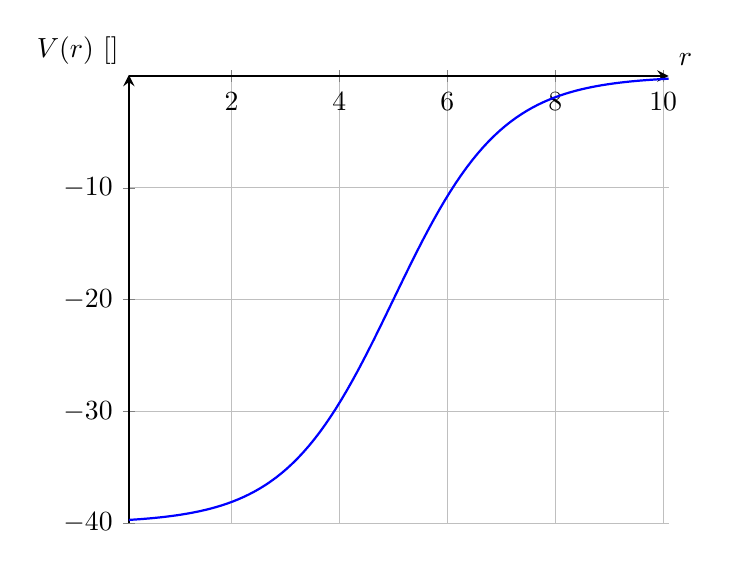
\begin{tikzpicture}
		\begin{axis}[
			domain=0.1:10.1,    % Rango del dominio para r > 0
			samples=100,    % Número de muestras para hacer la curva suave
			axis lines=middle,    % Líneas del eje
			xlabel={$r$},    % Etiqueta del eje x
			ylabel={$V(r) \ [\unit{\MeV}]$},    % Etiqueta del eje y
			ymin=-40.0, ymax=0.1,  % Límites del eje y
			xtick={2,4,6,8,10},       % Marcar el punto r=1
			ytick={-10,-20,-30,-40},      % Marcar el valor V(r) en r=1
			xlabel style={above right},
			ylabel style={above left},
			grid=both,
			thick
			]
			\addplot[
			blue,
			thick
			] {-(40/(1+exp(x-5)))};  % Punto de referencia
		\end{axis}
		
%		\draw[thick] (1.75,6.1) -- (5.2,6.1);
	%	\node (A) at (3.8,6.4) {$S_{\text{thick}}$};
	\end{tikzpicture}
	\caption{Potencial Wood-Saxon, variables de distancia en coordenadas reducidas ($R = 5, \ a = 1$).}	
	\label{Fig:04-02}
\end{figure}

\subsection{Interacción espín-órbita}

En los años 40 del siglo XX se realizaron muchos esfuerzos para construir un modelo de estructura nuclear que explicase de los números mágicos. En 1949 Mayer, Haxel, Suess y Jensen probaron que la inclusión de un potencial de interacción espín-órbita producía el desdoblamiento correcto de los subniveles en las capas. En física atómica la interacción espín órbita tiene su origen en la interacción del momento dipolar magnético creado por el espín del electrón con el campo mangnético que el electrón ve en su propio sistema de referencia\footnote{En el sistema de referencia en que el electrón está en reposo y el núcleo atómico está en movimiento y genera un campo magnético que interacciona con el momento dipolar magnético del electrón.}; los efectos aquí son típicamente del orden de una parte entre $10^5$, demasiado pequeños como para generar un desdoblamiento energético que modifique los \textit{números mágicos atómicos}. En el caso del nuúleo veremos que la interacción espín-órbita si introduce cambios significativos en lo que concierne a la secuencia de números mágicos. 

Introducimos entonces una interacción espín-órbita en el potencial nuclear de la siguiente manera:

\begin{equation}
    V(r) \longrightarrow V(r) + V_{so} (r) \parentesis{\lnn \cdot \sn}
\end{equation}
El factor $V_{so} (r)$ no es el más importante aquí, el que causa el desdoblamiento es el término $\lnn\cdot\sn$. Los estados de cada partícula se tienen que etiquetar ahora como el número cuántico correspondiente al momento angular total $\jn =\lnn+\sn$. Como los nucleones tienen $s=1/2$, los posibles valores de $j$ para un nucleón son $j=\ell\pm 1/2$, excepto para $\ell=0$ que solo es posible $j=1/2$. Podemos calcular el valor esperado de la expresión $\lnn \cdot \sn$ como:

\begin{equation}
    \jn^2 = \lnn^2 + 2 \lnn\cdot\sn + \sn^2 \Rightarrow \lnn \cdot \sn = \frac{1}{2} \parentesis{\jn^2 -\lnn^2 -\sn^2}     
\end{equation}
\begin{equation}
    \langle \lnnn \cdot \sn \rangle = \frac{\hbar^2}{2} \ccorchetes{j(j+1)-\ell(\ell+1) - s(s-1)}
\end{equation}
Supongamos ahora el nivel $1f$ ($\ell = 3$), que tiene una degeneración total $2(2\ell+1)=14$ (a cada uno le corresponde una degeneración diferente). Los posibles valores de $j$ son $j=\ell \pm 1/2=5/2$ o $7/2$, lo que nos da los dos estados $1f_{5/2}$ y $1f_{7/2}$, que constituyen un doblete espín-órbita y están degenerados y están separados por una energía proporcional al valor de $\langle \lnn \cdot \sn \rangle$. Esto es, la diferencia de energía entre dos núcleos debido a la interacción espín órbita vendrá dada por:

\begin{equation}
	\Delta E = V_{SO} (r) \ccorchetes{\langle \lnn_1 \cdot \sn_1 \rangle - \langle \lnn_2 \cdot \sn_2 \rangle}
\end{equation}
Para cada uno de estos dos orbitales tenemos una degeneración $(2j+1)$ proveniente de los distintos valores que $m_j$ puede tomar, lo cual proporciona una capacidad de 6 estaos nucleares para el $1f_{5/2}$ y 8 para el $1f_{7/2}$. Un total de 14, que coincide con el número inicial (el número total de estados no puede cambiar). Para cada par de estados de un doblete espín órbita con $\ell \neq 0$ tenemos una energía de separación proporcional a

\begin{equation}
	\langle \lnn \cdot \sn \rangle_{j=\ell+1/2} - \langle \lnn \cdot \sn \rangle_{j=\ell-1/2} = \frac{\hbar^2}{2} (2\ell +1)
\end{equation}
La fórmula anterior implica que la separación energética aumenta a medida que crece $\ell$ . Si tomamos $V_{so} (r)$ negativo, el miembro del par con mayor $j$ se desplaza hacia abajo entre los niveles de la segunda y tercera capas. Los 8 nucleones que puede contener el orbital $1f_{7/2}$ se podrían añadir a los 20 de las tres primeras capas generando un número mágico 28. De manera análoga es posible generar todos los números mágicos observados. 

Existen varias secuencias de llenado de nucleones en la literatura, dependiendo de los parámetros exactos que se usen en la parametrización del campo nuclear autoconsciente. La que aparece en el libro de K. Krane (las barras verticales indican las separaciones entre capas que dan lugar a los números mágicos 2,8,28,50,82):

\begin{equation}
	\begin{array}{l}(1s_{1/2})^2 \ || \ (1p_{3/2})^4 (1p_{1/2})^2 \ || \ (1d_{5/2})^6 (2s_{1/2})^2 (1d_{3/2})^4 (1f_{7/2})^8 \ || \ (2p_{3/2})^4 \\ (1f_{5/2})^6 (2p_{1/2})^2 (1g_{9/2})^{10} \ || \ (1g_{7/2})^8 (2d_{5/2})^6 (2d_{3/2})^4 (3s_{1/2})^2 (1h_{11/2})^{12}    \ || \\ \ (1h_{9/2})^{10} (2f_{7/2})^8 (2f_{5/2})^6 (2p_{3/2})^4 (2p_{1/2})^2  (1i_{13/2})^{14} \ || \ (2g_{9/2})^{10} (3d_{5/2})^6 \\ (1i_{11/2})^{12}    (2g_{7/2})^8 (4s_{1/2})^2 (2d_{3/2})^4  (1j_{15/2})^{16} \ ||		\ldots
	\end{array}
\end{equation}
De tal modo que $(1p_{3/2})^4$ indica el primer llenado del orbital $p$ ($\ell=1$), con espín total $3/2$ ($j=\ell + s$) con degeneración total 4 (la degeneración es $2j+1$). 



\subsection{Modelos dipolares magnéticos}

En la versión extrema del modeleo de capas (\textit{one-particle shell model}), el momento dipolar magnético de un núcleo con $A$ impar está determinado por el momento dipolar magnético del último nucleón desapareado. Veamos cuál es el acuerdo que existe entre los datos experiementales y este modelo. Recordemos que el operador de momento magnético dipolar para un núcleo de $A$ nucleones se escribe como

\begin{equation}
	\mun = \frac{\mu_N}{\hbar} \sum_{i=1}^A \ccorchetes{g_i^{(\ell)} \lnn_i + g_i^{(s)}\sn_i} \tquad \mu_N = \frac{e\hbar}{2m_p}
\end{equation}
donde $\mu:N$ es el magnetón nuclear y los valores para los fotones o razones giromagnéticos correspondientes al momento angular orbital y al de espín, para el fotón neutrón y electrón son:

\begin{eqnarray}
	g_p^{(\ell)} = 1 & & g_p^{(s)} = \num{5.585694674} \\
	g_n^{(\ell)} = 0 & & g_p^{(s)} = \num{-3.8260854} \\
	g_e^{(\ell)} = -1 & & g_p^{(s)} = \num{2.002319304374} \\
\end{eqnarray}
El momento dipolar magnético del núcleo se define como el valor esperado de la tercera componente del operador $\mun$ en un estado nuclear en el que la proyección del momento angular sobre el eje $z$ es máxima, es decir, cuando $j_z=j\hbar$. En la versión extrema del modelo de capas se pretende explicar el momento magnético nuclear como originado por el único nucleón desapareado (sólo para núcleos de $A$ impar). Considerando entonces la contribución de un único nucleón, la tercera componente del operador anterior es:

\begin{equation}
	\mu_z = \frac{\mu_N}{\hbar} \parentesis{g^{(\ell)} \ell_z + g^{(s)} s_z}
\end{equation}
La presencia de interacción espín-órbita implica que el potencial es no central, y por lo tanto los autoestados del hamiltoniano no lo serán también del operador momento angular orbital, sino del momento angular total. Esto quiere deecir que $\ell_z$ y $s_z$ ya no serán \textit{buenos} números cuánticos, hemos de usar $\jn=\lnn+\sn$ y $j_z$. Podemos reescribir la expresión anterior usado la tercera componente de $\kn$ de la siguiente manera (recordando que $\j_z=\ell_z + s_z$):

\begin{equation}
	\mu_z = \frac{\mu_N}{\hbar} \ccorchetes{g^{(\ell)}j_z + (g^{(s)}-g^{(\ell)})  s_z}
\end{equation}
Tomamos el valor esperado de la experiencia anterior cuando $j_z=j\hbar$, y para aligerar notación preescidimos del subíndice $z$ y $\mu$ sobreentendiendo que se trata de la tercera componente:
\begin{equation}
	\langle \mu_z \rangle = \frac{\mu_N}{\hbar} \ccorchetes{g^{(\ell)} \langle j_z \rangle + (g^{(s)}-g^{(\ell)}) \langle s_z \rangle}
\end{equation}
Obtenemos así de nuevo estas dos expresiones para el momento dipolar magnético:

\begin{eqnarray}
	\mu_{j=\ell+\frac{1}{2}} & = & \frac{\mu_N}{2} \ccorchetes{(2j+1)g^{(\ell)} + g^{(s)}} \\
	\mu_{j=\ell-\frac{1}{2}} & = & \frac{\mu_N}{2} \frac{j}{j+1} \ccorchetes{(2j+1)g^{(l)} - g^{(s)} }
\end{eqnarray}

\section{Modos colectivos}

Para los núcleos par-par el modelo de capas predice que el estado fundamental es un $0^+$ y las características del espectro de los estados excitados deberían quedar determinadas por la excitación de una sola partícula. Examinemos por ejemplo el $\ce{^130_50 Sn_80}$. Tiene un número mágico de protones (50), y el final de su llenado es $\ldots(1f_{5/2})^6 (2p_{1/2})^2 (1g_{9/2})^{10}$, mientras que el final de llenado de los neutrones es $\ldots(2d_{3/2})^4(3s_{1/2})^2(1h_{11/2})^10$, lo totaliza 80 neutrones, faltando dos para llenar el orbital $1h_{11/2}$ (tiene 12 ya que su degeneración es $2\cdot 11/2+1$). Para formar un estado excitado podríamos pensar en romper una de las parejas de neutrones $1h_{11/2}$ y pasar un neutrón al primer orbital de la siguiente capa, el $1h_{9/2}$; o bien romper una pareja de protones y enviar un protón al orbital $1g_{7/2}$. En ambos casos necesitamos mucha energía para salvar la distancia entre dos capas, de tal manera que los estados excitados más bajos deben provenir de excitaciones de los neutrones dentro de la última capa semillena. Podríamos formar un estado excitado rompiendo una pareja de neutrones del orbital $3s_{1/2}$ y el llevando un neutrón al orbital $1h_{11/2}$. Las propiedades de este estado excitado estarían determinadas esencialmente por el acoplamiento del neutrón desapareado del orbital $3s_{1/2}$ y el desapareado del $h_{11/2}$. Tendríamos que acoplar sus momentos angulares totales y obtendríamos $|j_1-j_2|\leq j \leq (j_1+j_2)$, es decir $j=5,6$. Otra posibilidad sería romper una pareja del orbital $2d_{3/2}$ lo que proporcionaría $j=4,5,6,7$. A los orbitales $3s_{1/2}$ y $2d_{3/2}$ les corresponde paridad positiva ($\ell = 0$ y $\ell = 2$), mientras que al orbital $1h_{11/2}$ le corresponde paridad negativa ($\ell = 5$), por lo tanto todos los acoplamientos anteriores proporcionan estados excitados de paridad negativa. Examinando el espectro $\ce{^{130}_{50} Sn_80}$ vemos efectivamente algunos estados excitados de paridad negativa, con espín en el rango 4-7 y energías entorno a 2 MeV, características de la ruptura de una pareja de nucleones. 

Otra manera de generar estados excitados en el $\ce{^130_50 Sn_80}$ consistiría en acoplar una de las parejas de neutrones del orbital $1h_{11/2}$ a un momento angular total distinto de cero. El momento angular resultante estaría entre $11$ y $0$\footnote{Ya que $11/2+11/2=11$ y $11/2-11/2=0$}. Por otro lado, la función de ondas total del sistema formado por estos nucleones debe ser completamente antisimétrica, porque se trata de fermiones idénticos, y en este caso la antisimetrización nos llevaría a eliminar todos los valores impares del momento angular total resultante y quedarnos sólo con los pares. Así deduciríamos que los posibles valores de espín nuclear generados por el acoplamiento de dos nucleones con $j=11/2$ son $0^+,2^+,4^+,6^+,8^+,10^+$. De nuevo, en el espectro del $\ce{^130_50 Sn_80}$ vemos algunos candidatos con estas características a una energía entorno a 2 MeV. El modelo de capas parece funcionar razonablemente bien para estos casos. Sin embargo hay un primer nivel excitado $2^+$ a una energía de alrededor de 1.2 MeV que no puede ser explicado a partir de consideraciones similares a los anteriores.

Una característica común a todos los núcleos par-par es la existencia de un primer estado excitado $2^+$ con una energía del orden de la mitad de la que sería necesaria para deshacer una pareja de nucleones. Esto no se puede explicar en términos del comportamiento individual de los nucleones, sino que parece más bien una propiedad colectiva de todos los núcleos par-par. Examinaremos en lo que sigue los grados de libertad colectivos de los núcleos. Los grados de libertad colectivos están asociados con las propiedades colectivas que varían suavemente con el número másico $A$, a diferencia de las propiedades que surgen del comportamiento individual de los nucleones. Cuatro de estad propiedades colectivas son:

\begin{itemize}
	\item La energía del estado excitado $2^+$ más najo. Esta energía $E(2^+)$ decrece gradualmente en función de $A$ excepto en las regiones cercanas a la clausura de una capa.
	\item El cociente $E(4^+)/E(2^+)$ para los estados excitados nucleares $2^+$ y $4^+$. El valor de esta razón es aproximadamente 2.0 para núclos con $A<150$ pero excepcionalmente constante e igual a 3.3 para $150<A<190$ y $230<A$. 
	\item Los momentos dipolares magnéticos de los estados excitados $2^+$ más bajos, son aproximadamente constantes y caen en el rango de 0.7 y 0.1 magnetones nucleares.
	\item Los momentos cuadrupolares eléctricos de los estados excitados $2^+$ más bajos. Son pequeños para  $A<150$ y muy grandes para $A>150$.
\end{itemize}
Esto sugiere que los núcleos con $A>150$ tienen una serie de propiedades colectivas diferentes a los núcleos con $150<A<190$. Las propiedades colectivas de los nucleos de la primera clase se estudian usualmente mediante modelos basados en vibraciones en torno a una forma nuclear esférica, mientras que los núcleos con $150<A<190$ muentras características típicas de rotaciones en un sistema nó esférico. Vibraciones y rotaciones son las dos grandes clases de movimientos colectivos nucleares. El modelo colectivo también se suele denominar el modelo de la gota líquida.

\newpage

% ----------------------------
% Ejercicios 
% ----------------------------

\section*{Ejercicios}
\addcontentsline{toc}{section}{\textit{Ejercicios}}


%---------------------------
% Ejercicio 1
%---------------------------

\begin{Enunciado}
\subsection*{Ejercicio 1} 
%%\addcontentsline{toc}{subsection}{Ejercicio 1}

Para un transistor P\textsuperscript{+}NP de silicio representar aproximadamente:
\begin{enumerate}[label=\alph*)]
    \item Bajo equilibrio las bandas, el campo eléctrico, la densidad de carga y el potencial.
    \item Las bandas en los casos de activa, corte, saturación y activa inversa.
    \item Los portadores en los casos de activa, corte, saturación y activa inversa.
\end{enumerate}
\end{Enunciado}

\vspace*{1em}

\lipsum[1].

\vspace*{2em}


%---------------------------
% Ejercicio 2
%---------------------------

\begin{Enunciado}
\subsection*{Ejercicio 2} 
%\addcontentsline{toc}{subsection}{Ejercicio 2}

Para un transistor de GaAs tipo PNP, con concentraciones $1.0 \times 10^{16}$, $5.0 \times 10^{15}$ y $1.0 \times 10^{15}$ cm\textsuperscript{-3}, con un ancho de emisor, base y colector de 20, 2 y 50 micras respectivamente, usando la aproximación de vaciamiento en los siguientes casos:
    \begin{enumerate}[label=\alph*)]
        \item Representar las bandas y el campo eléctrico en equilibrio.
        \item Representar las bandas y el campo eléctrico cuando se polariza $V_{EB} = 0.8$ V y $V_{CB} = -1.5$ V.
    \end{enumerate}
\textbf{Datos:} concentración intrínseca $2.25 \times 10^6$ cm\textsuperscript{-3}, gap de energía 1.42 eV, masa del electrón 0.066 y de hueco 0.52, permitividad relativa: 12.9, permitividad absoluta del vacío: $8.85 \times 10^{-14}$ F/cm.
\end{Enunciado}

\vspace*{1em}

Solucion: 

\begin{enumerate}[label=\alph*)]
    \item Primero vamos a presentar los valores de lal gráfico de bandas y el campo eléctrico en el equilibrio. Para esto tenemos que usar las típicas ecuaiones que hemos usado en todos los temas anteriores, y que por tanto no vamos a reptir (véase \ref{Sec:03-02}). Ahora si, tenemos algunos resultados que si tenemos que representar, que son $x_n',x_p',x_n'',x_p'',\Vbi',\Vbi''$. Recordanos que $x_n$ y $x_p$ caen con $N_D,N_A$.  Nosotros llamamos \textit{prima} a cualquier parámetro de emisor-base (EB) y \textit{doble prima} a cualquier parámetro de base-colector (BC). Así pues:
    \begin{equation}
        \text{EB:} \ x_n'=51.94 \ \mu \unit{m} \quad  x_p'=25.97  \mu \unit{m} \quad \Vbi'=1.13 \ \unit{V}
    \end{equation}
    \begin{equation}
        \text{BC:} \ x_n''=28.09 \ \mu \unit{m} \quad  x_p''=122.64  \mu \unit{m} \quad \Vbi'= 1.071 \ \unit{V}
    \end{equation}
    Y el campo eléctrico máximo
    \begin{equation}
       \abs{\Ecal'}_{\max}''=28200 \ \unit{V/cm} \quad  
       \abs{\Ecal''}_{\max}''=14100 \ \unit{V/cm} 
    \end{equation}

    \begin{center}
        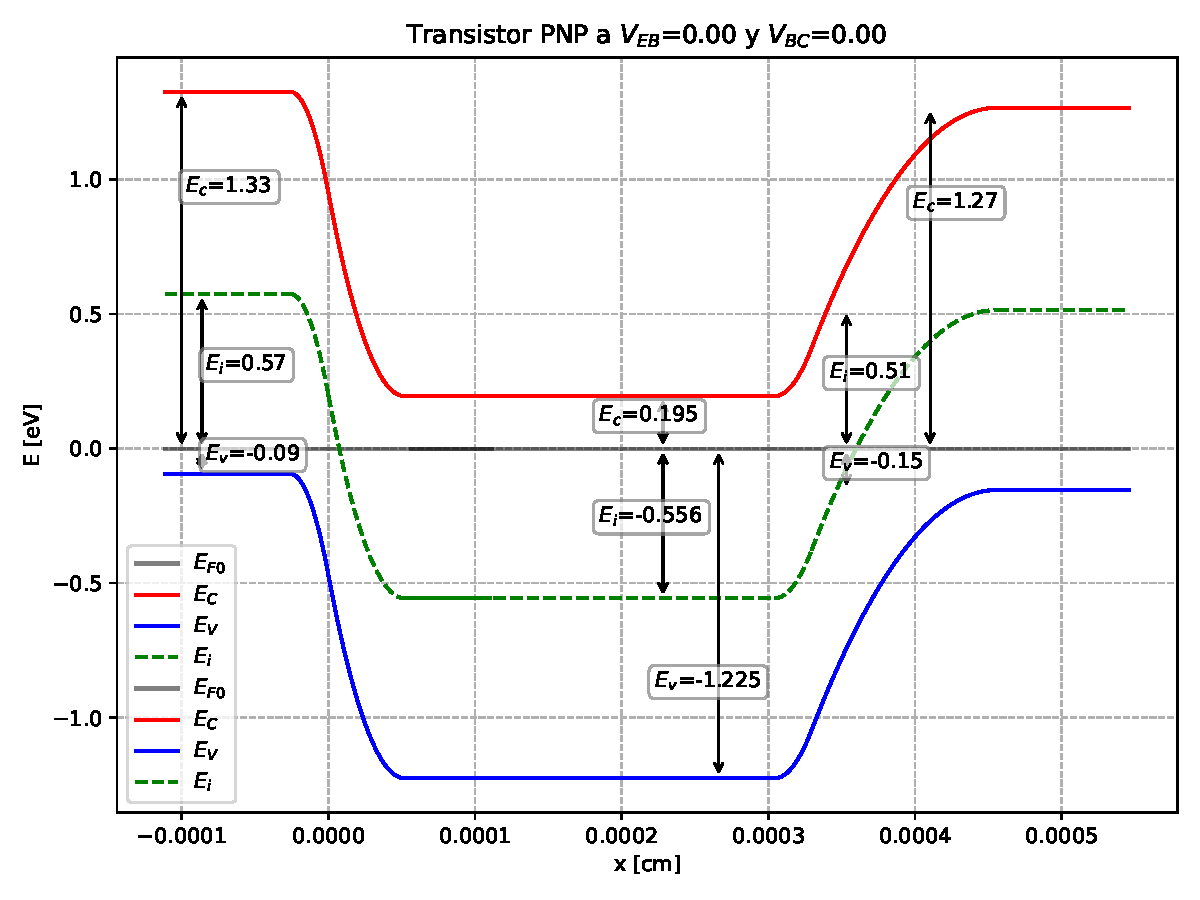
\includegraphics[width=0.48\linewidth]{Ejercicios/Ch_04/04_Ejercicio-2-01.pdf} \hfill
        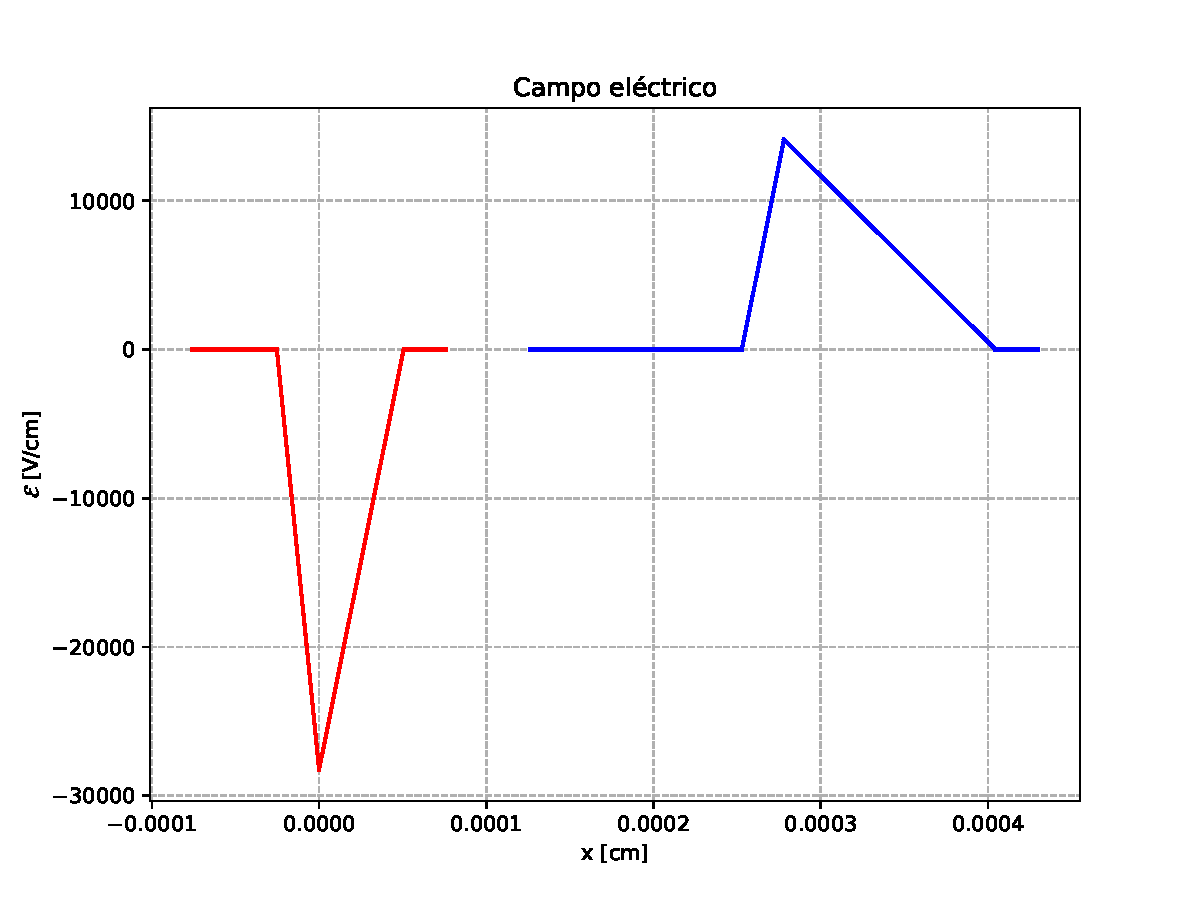
\includegraphics[width=0.48\linewidth]{Ejercicios/Ch_04/04_Ejercicio-2-03.pdf}
    \end{center}
    \item Para la segunda tenemos que calcular los mismos paráemtros pero con polarizaciones
    \begin{equation}
        \text{EB:} \ x_n'=28.09 \ \mu \unit{m} \quad  x_p'=14.05  \mu \unit{m} \quad \Vbi'=1.13 \ \unit{V}
    \end{equation}
    \begin{equation}
        \text{BC:} \ x_n''=39.16 \ \mu \unit{m} \quad  x_p''=122.64  \mu \unit{m} \quad \Vbi'= 195.8 \ \unit{V}
    \end{equation}
    \noindent Y el campo eléctrico máximo
    \begin{equation}
       \abs{\Ecal'}_{\max}''=14200 \ \unit{V/cm} \quad  
       \abs{\Ecal''}_{\max}''=21900 \ \unit{V/cm} 
    \end{equation}
    \begin{figure}[h!] \centering
        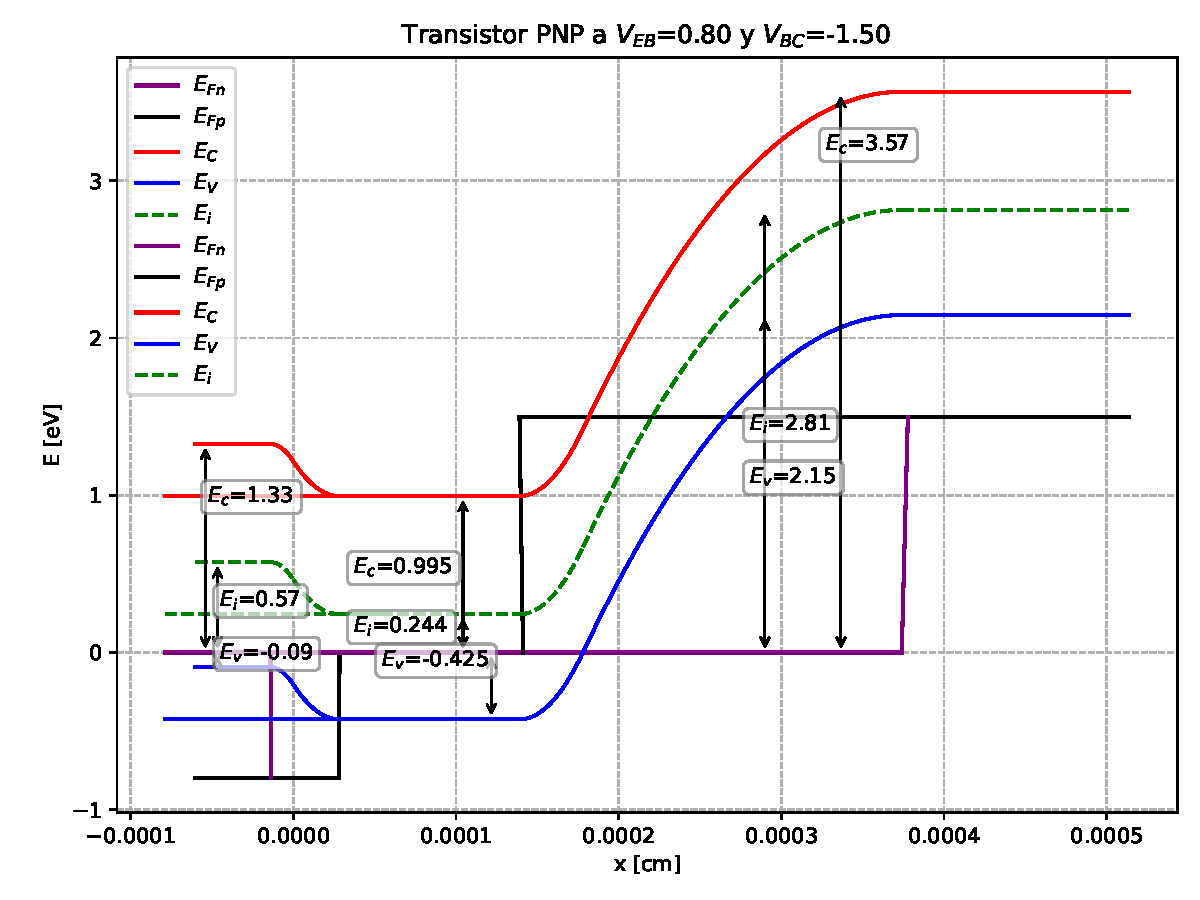
\includegraphics[width=0.48\linewidth]{Ejercicios/Ch_04/04_Ejercicio-2-02.pdf} \hfill
        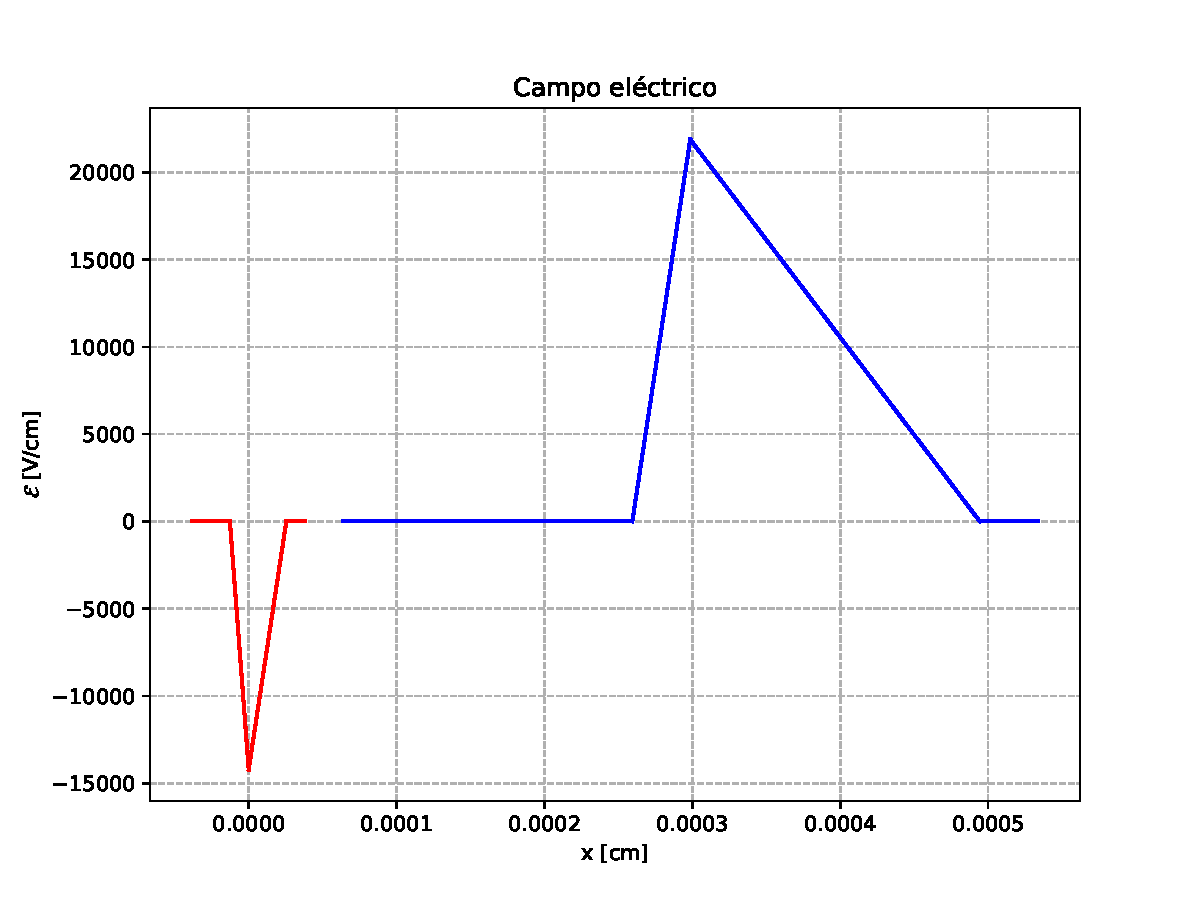
\includegraphics[width=0.48\linewidth]{Ejercicios/Ch_04/04_Ejercicio-2-04.pdf}
        \caption{Imagenes apartado b).}
    \end{figure}

\end{enumerate}
\vspace*{2em}

%---------------------------
% Ejercicio 3
%---------------------------

\begin{Enunciado}
\subsection*{Ejercicio 3}
%\addcontentsline{toc}{subsection}{Ejercicio 3}


Tenemos un PNP de silicio con concentraciones $5 \times 10^{18}$, $3 \times 10^{17}$ y $1 \times 10^{16}$ cm\textsuperscript{-3}, con un ancho de emisor, base y colector de 20, 2 y 30 micras, y con un área de 1 cm\textsuperscript{2}. Cuando se polariza la unión emisor-base en directa con 0.5 voltios y la unión base-colector en inversa con 2 voltios, calcular y representar:
\begin{enumerate}[label=\alph*)]
    \item Las bandas bajo esa polarización.
    \item La concentración de minoritarios en el dispositivo.
    \item Calcular el valor de todas las componentes de corriente (suponiendo que no hay recombinación en la base), y representarlas gráficamente.
\end{enumerate}
\textbf{Datos:} concentración intrínseca $9.6 \times 10^9$ cm\textsuperscript{-3}, gap de energía 1.12 eV, masa del electrón 1.18 y de hueco 0.812, permitividad relativa: 11.8, permitividad del vacío: $8.85 \times 10^{-14}$ F/cm, coeficiente de difusión y tiempo de vida de emisor, base y colector de 52, 40 y 115 cm\textsuperscript{2}/s, y $10^{-8}$, $10^{-7}$ y $10^{-6}$ segundos.
\end{Enunciado}

\vspace*{1em}

\lipsum[1].

\vspace*{2em}

%---------------------------
% Ejercicio 4
%---------------------------

\begin{Enunciado}
\subsection*{Ejercicio 4} 
%\addcontentsline{toc}{subsection}{Ejercicio 4}

\lipsum[1].
\end{Enunciado}

\vspace*{1em}

\lipsum[1].

\vspace*{2em}
%---------------------------
% Ejercicio 5
%---------------------------

\begin{Enunciado}
\subsection*{Ejercicio 5}
%\addcontentsline{toc}{subsection}{Ejercicio 5}

\lipsum[1].
\end{Enunciado}

\vspace*{1em}
    
\lipsum[1]

\vspace*{2em}

%---------------------------
% Ejercicio 6
%---------------------------

\begin{Enunciado}
\subsection*{Ejercicio 6}
%\addcontentsline{toc}{subsection}{Ejercicio 6}

\lipsum[1].
\end{Enunciado}

\vspace*{1em}

\lipsum[1].
    
\vspace*{2em}

\chapter{El transistor MOSFET}
\newpage

\section*{Ejercicios}
\addcontentsline{toc}{section}{\textit{Ejercicios}}



%---------------------------
% Ejercicio 1   
%---------------------------
\begin{Enunciado}
	\subsection*{Ejercicio 1}
	%\addcontentsline{toc}{subsection}{\textit{Ejercicio 1}}

	Indicar la condición de polarización y dibujar los diagramas de bandas de enerǵia y densidad de carga para un MOS ideal de silicio en las isugientes condiciones:

	\begin{enumerate}[label=\alph*)]
		\item $\phi_B= \SI{0.312}{V}$  y  $\phi_S= \SI{0.312}{V}$.
		\item $\phi_B= -\SI{0.234}{V}$  y  $\phi_S= \SI{0.078}{V}$.
		\item $\phi_B= -\SI{0.234}{V}$  y  $\phi_S= -\SI{0.468}{V}$.
		\item $\phi_B= \SI{0.390}{V}$  y  $\phi_S= \SI{0.936}{V}$.
	\end{enumerate}
\end{Enunciado}

\vspace*{1em}

Indicar la condición de polarización es indicar básicamente si está en acumulación $(\phi_S<0)$, en plana $(\phi_S=0)$, en vaciamiento $(\phi_S>0$) o en inversa $(\phi_S>2\phi_F$).

Por definición los valores de $\phi_B$ y $\phi_S$ son:

\begin{equation*}
	\phi_F \equiv \phi_B \equiv E_i(\text{sustrato}) - E_F \tquad
	\phi_S \equiv E_i(\text{sustrato}) - E_i (\text{interfaz})
\end{equation*}
Por lo tanto, para determinar el tipo de semiconductor debemos usar, debemos observar el signo de $\phi_B$. Si $\phi_B > 0$, el semiconductor es de tipo p, y si $\phi_B < 0$, el semiconductor es de tipo n. Esto se debe a que $\phi_B$ está relacionado con la posición del nivel de Fermi respecto al nivel intrínseco.
\begin{itemize}
	\item Si $\phi_B > 0$, el nivel de Fermi está por debajo del nivel intrínseco, indicando un semiconductor tipo p.
	\item Si $\phi_B < 0$, el nivel de Fermi está por encima del nivel intrínseco, indicando un semiconductor tipo n.
\end{itemize}
Con esta información, podemos determinar tanto la condición de polarización como el tipo de semiconductor para cada caso. Esto será importante ya que nos dirá que carga en la interfaz (si la del metal o la del semiconductor) es postiiva o negativa.


\begin{enumerate}[label=\alph*)]
	\item Estamos ante un semiconductor tipo $P$, en la región de vaciamiento o intrínseco (ya que $\phi_S =  \phi_F$).
	      \begin{figure}[H]\centering
		      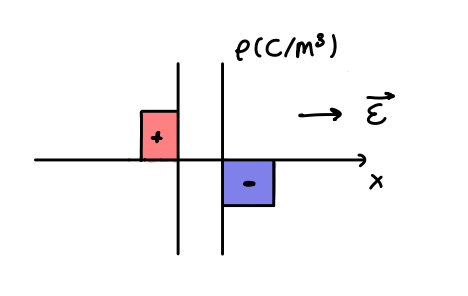
\includegraphics[width=0.45\linewidth]{Ejercicios/Ch_05/Ej_01_a1.png} \hfill
		      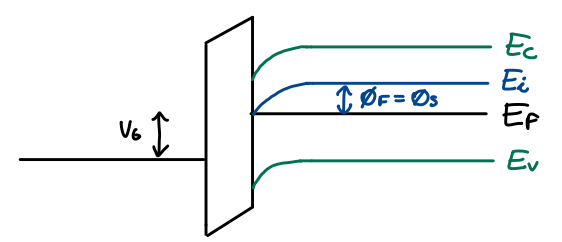
\includegraphics[width=0.45\linewidth]{Ejercicios/Ch_05/Ej_01_a2.png}
	      \end{figure}
	\item Estamos ante un semiconductor tipo $N$ en la región de acumulación.
	      \begin{figure}[H]\centering
		      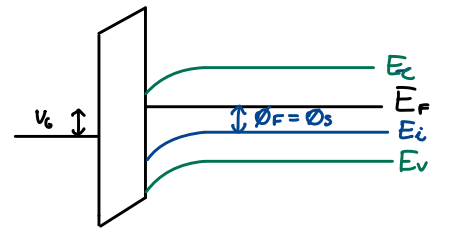
\includegraphics[width=0.45\linewidth]{Ejercicios/Ch_05/Ej_01_b1.png} \hfill
		      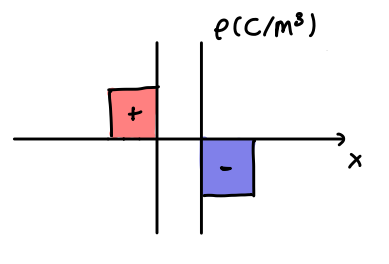
\includegraphics[width=0.45\linewidth]{Ejercicios/Ch_05/Ej_01_b2.png}
	      \end{figure}
	\item Estamos ante un semiconductor tipo $N$ en la región de transición entre vaciamiento e inversión ($\phi_S=2\phi_F$).

	      \begin{figure}[H]\centering
		      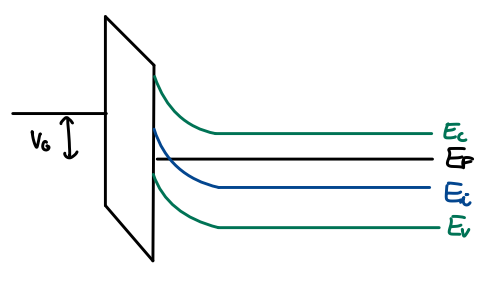
\includegraphics[width=0.45\linewidth]{Ejercicios/Ch_05/Ej_01_c1.png} \hfill
		      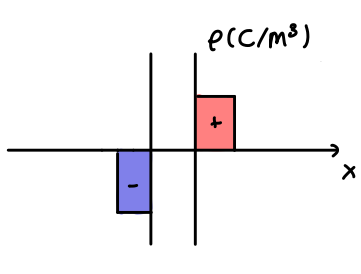
\includegraphics[width=0.45\linewidth]{Ejercicios/Ch_05/Ej_01_c2.png}
	      \end{figure}
	\item Estamos ante un semiconductor tipo $P$ en la región de inversión.

	      \begin{figure}[H]\centering
		      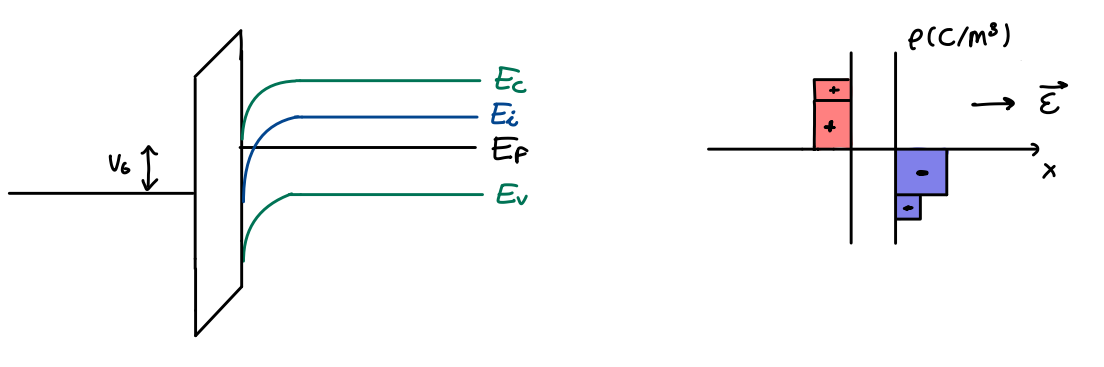
\includegraphics[width=0.9\linewidth]{Ejercicios/Ch_05/Ej_01_d.png}
	      \end{figure}
\end{enumerate}

\vspace*{2em}

%---------------------------
% Ejercicio 2
%---------------------------

\begin{Enunciado}
	\subsection*{Ejercicio 2}
	%\addcontentsline{toc}{subsection}{\textit{Ejercicio 2}}
	Un MOS ideal se mantiene constante a una temperatura $T=300$ K con $x_0=\SI{0.1}{\mu m}$ con un dopado del Si de $N_A=\SI{1e15}{cm^{-3}}$ (la constante dieléctrica relativa para el óxido es de 3.9). Calcula y representa:
	\begin{enumerate}[label=\alph*)]
		\item $\phi_B \equiv \phi_F$ y la anchura de la región de vaciamiento cuando $\phi_B = \phi_S$
		\item El campo eléctrico y la tensión aplicada en la puerta cuando $\phi_B = \psi_S$.
	\end{enumerate}
\end{Enunciado}

\vspace*{1em}

Las soluciones son, por apartado:

\begin{enumerate}[label=\alph*)]
	\item Conociendo $N_A$ y que $T=300$K podemos obtner $\phi_B = \phi_F$ ($n_i \approx \SI{1e10}{cm^{-3}}$ a 300 K). Luego como concemos $\phi_S$ en virtud de $\phi_B = \phi_S$, el cálculo de la anchura será trivial ya qie la solo depende de $\phi_S$.

	      \begin{equation*}
		      \phi_S = \phi_F = \frac{1}{q} \parentesis{E_i(\text{sustrato})-E_F} = \frac{kT}{q} \log \parentesis{\frac{N_A}{n_i}} \qquad
		      \phi_{S} = \SI{2.98e-01}{V}
	      \end{equation*}
	      tal que

	      \begin{equation*}
		      W = \sqrt{\frac{2\phi_S K_S \epsilon_0}{qN_A}} \qquad
		      W = \SI{6.24e-05}{cm}
	      \end{equation*}

	\item El campo elećtrico también se puede calcular facilmente, ya que en la zona S solo depende de $W$ (y de $N_A$ y $K_{S}$) y en la zona O depende de $\Ecal_{sc}$ en la interfaz y de las permitividades relativas. Al suponer metal perfecto no hay campo elećtrico en el metal. Veamos que:

	      \begin{equation*}
		      \Ecal_S (x) = \left\lbrace \begin{array}{ll}
			      \frac{qN_A}{K_S \epsilon_0} (W-x) & \quad \text{si} \ 0\leq x \leq W \\
			      0                                 & \quad \text{si} \ W<x
		      \end{array} \right.
	      \end{equation*}
	      Luego la tensión aplicada también la podemos calcular facilmente a través de las fórmulas:

	      \begin{equation*}
		      V_G = \phi_S + \frac{K_S}{K_o} x_o \sqrt{\frac{2qN_A}{K_S\epsilon_0} \phi_s}
	      \end{equation*}
	      Las soluciones son:

	      \begin{equation*}
		      \Ecal(0) = \SI{6.96e+03}{V/cm} \qquad
		      V_G = \SI{5.85e-01}{V}
	      \end{equation*}

	      	\begin{figure}[H]\centering
		      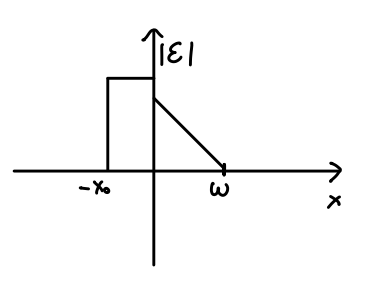
\includegraphics[width=0.45\linewidth]{Ejercicios/Ch_05/Ej_02_a.png} \hfill
		      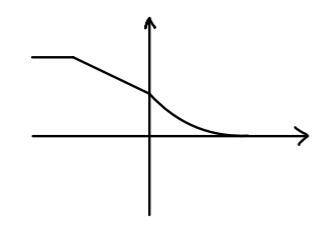
\includegraphics[width=0.45\linewidth]{Ejercicios/Ch_05/Ej_02_c.png}
			\centering\end{figure}

			Aunque no nos lo piden, las bandas dibujadas:
			\begin{figure}[H]\centering
				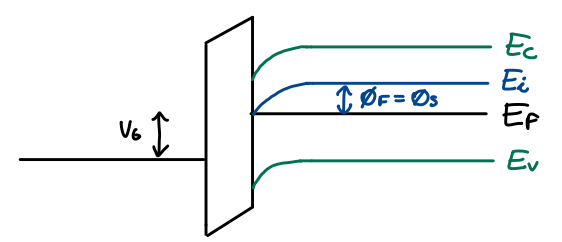
\includegraphics[width=0.45\linewidth]{Ejercicios/Ch_05/Ej_02_b.png}
			  \centering\end{figure}
  

\end{enumerate}



\vspace*{2em}

%---------------------------
% Ejercicio 3
%---------------------------

\begin{Enunciado}
	\subsection*{Ejercicio 3}
	%\addcontentsline{toc}{subsection}{\textit{Ejercicio 3}}
	Dibujar la distribución de carga, de campo eléctrico y de potencial en un MOS ideal con sustrato tipo N bajo condiciones de acumulación, vaciamiento e inversión (incluir en la representación las tres zonas que componen el dispositivo: metal, óxido y semiconductor). Considerando una puerta de polisilicio de tipo N, un espesor de óxido de silicio de 50 nm con constante dieléctrica relativa par el óxido de 3.9 y con un dopado de $N_D = \SI{5.0e16}{cm^{-3}}$, calcula:
	\begin{enumerate}[label=\alph*)]
		\item Capacidad del óxido. 
		\item Tensión de banda plana.
		\item Tensión umbral ideal.
		\item Tensión umbral real. 
	\end{enumerate}
\end{Enunciado}

\vspace*{1em}

	En primer lugar nos mandan dibujar las gráficas de: distribución de carga, campo eléctrico y potencial en el MOS ideal de sustrato N para los 3 casos típicos: acumulación, vaciamiento e inversión. Así pues: 
	\begin{itemize}
		\item Acumulación:
		\begin{figure}[H]\centering
			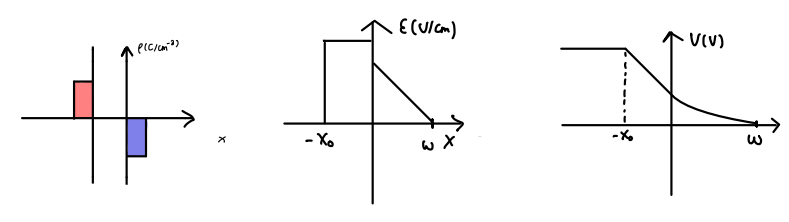
\includegraphics[width=0.8\linewidth]{Ejercicios/Ch_05/Ej_03_a1.png}
		\end{figure}
		\item Vaciamiento:
		\begin{figure}[H]\centering
			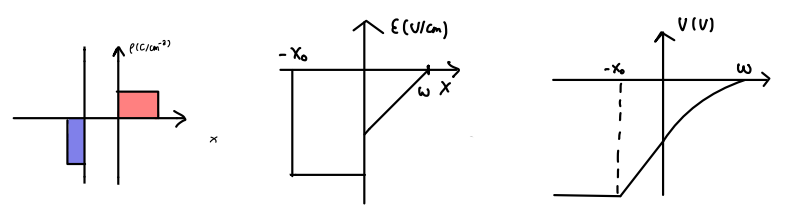
\includegraphics[width=0.8\linewidth]{Ejercicios/Ch_05/Ej_03_a2.png}
		\end{figure}
		\item Inversión:
		\begin{figure}[H]\centering
			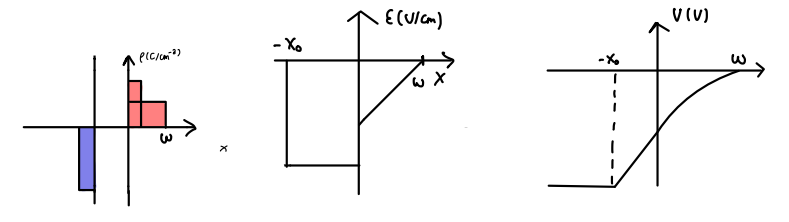
\includegraphics[width=0.8\linewidth]{Ejercicios/Ch_05/Ej_03_a3.png}
		\end{figure}
	\end{itemize}


\begin{enumerate}[label=\alph*)]
	\item Para calcular la capacidad del óxido solo tenemos que hacer: 
\end{enumerate}


%---------------------------
% Ejercicio 4
%---------------------------

\begin{Enunciado}
	\subsection*{Ejercicio 4}
	%\addcontentsline{toc}{subsection}{\textit{Ejercicio 4}}

	Para un dispositivo MOS SiO$_2$-Si ideal con espesor de óxiddo de 5 nm, $N_A = \SI{1e17}{cm^{-3}}$ y una constante dieléctrica relativa para el óxido de 3.9, calcula y representa la tensión de puerta y el campo elećtrico de la interfaz necesarios para que el Silicio en la interfaz se comporte como un intrínseco.
\end{Enunciado}

Recordamos que para que el silicio en la interfaz se comporte como un intrínseco debe verificarse que:

\begin{equation*}
	E_i(\text{interfaz}) - E_F = 0
\end{equation*}
es decir, que:

\begin{equation*}
	\phi_S = \phi_F \qquad
	\phi_{S} = \SI{4.17e-01}{V}
\end{equation*}
ya que

\begin{equation*}
	\phi_F \equiv \phi_B \equiv E_i(\text{sustrato}) - E_F \tquad
	\phi_S \equiv E_i(\text{sustrato}) - E_i (\text{interfaz})
\end{equation*}
Entonceses trivial el cálculo de la tensión de puerta $V_G$ y $\Ecal(\text{interfaz})$, ya que es simplemente aplicar las ecuaciones:

\begin{equation*}
	W = \sqrt{\frac{\phi_S K_S \epsilon_0}{qN_A}}
\end{equation*}
\begin{equation*}
	\Ecal_S (\text{interfaz}) = \frac{qN_A}{K_S \epsilon_0}W
\end{equation*}
\begin{equation*}
	V_G = \phi_S + \frac{K_S}{K_o} x_o \sqrt{\frac{2qN_A}{K_S\epsilon_0} \phi_s}
\end{equation*}
Así pues:

\begin{equation*}
	W = \SI{7.34e-06}{cm} \quad
	E(0) = \SI{1.14e+05}{V/cm} \quad 
	V_G = \SI{5.87e-01}{V}
\end{equation*}
\begin{figure}[H] \centering
	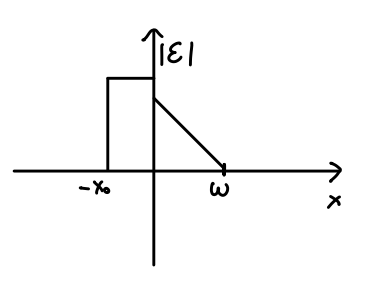
\includegraphics[width=0.45\linewidth]{Ejercicios/Ch_05/Ej_04_a.png} \hfill
	\includegraphics[width=0.45\linewidth]{Ejercicios/Ch_05/Ej_04_b.png}
\end{figure}

\vspace*{2em}
%---------------------------
% Ejercicio 5
%---------------------------

\begin{Enunciado}
	\subsection*{Ejercicio 5}
	%\addcontentsline{toc}{subsection}{\textit{Ejercicio 5}}
	La concentración de electrones en los contactos de fuente y drenador de un MOSFET de silicio es de $\SI{1e+17}{cm^{-3}}$, y la tensión aplicada bajo la puerta hace que la concetración de electroens sea de $\SI{1e+9}{cm^{-3}}$. Si suponemos que la corriente qeu fluye es despreciable, calcula y representa la barrera que ven los portadores. 
\end{Enunciado}

\vspace*{1em}

	Como sabemos, $n=\SI{1e+9}{cm^{-3}}$ es menor que $n_i =\SI{1e+10}{cm^{-3}}$, por lo que la región entre fuente y drenador es de tipo P. Teniendo en cuenta que nos dicen que la corriente es despreciable, esto es, el nivel de Fermi es constante, podemos hacer un dibujo de las bandas, aunque de manera esquemática (recordemos que en realidad en la zona de vaciamiento se curvan,  no son líneas rectas):

\begin{figure}[H] \centering
	\includegraphics[width=0.45\linewidth]{Ejercicios/Ch_05/Ej_05.png} \hfill
\end{figure}

	De lo que se puede deducir que el salto $\Vbi$ es:

	\begin{equation}
		E_i|_P - E_i|_{N^+} =  - kT \log \parentesis{\frac{n_P}{n_i}} - kT  \log \parentesis{\frac{n_N}{n_i}}  = 0.059264 + 0.41668 \ \eV = 0.4789 \ \eV 
	\end{equation}


\vspace*{2em}

%---------------------------
% Ejercicio 6
%---------------------------

\begin{Enunciado}
	\subsection*{Ejercicio 6}
	%\addcontentsline{toc}{subsection}{\textit{Ejercicio 6}}
	Para un MOSFET con puerta de polisilicio tipo N y canal tipo n de silicio con un espesor de la capa de óxido de 50 nm, $N_A = \SI{5e16}{cm^{-3}}$, $\epsilon_{ox}=3.9$, $\epsilon_{Si} = 11.9$ y $\chi=4.05 \eV$, calcular:
	\begin{enumerate}[label=\alph*)]
		\item Capacidad del óxido, la tensión de la anda plana y la tensión umbral.
		\item Representa las bandas en equilibrio térmico.
		\item Representa la estructura de bandas y la densidad de carga cuando el MOS está en inversión, vaciamiento y en acumulación.
	\end{enumerate}
\end{Enunciado}

\vspace*{1em}
La solución es:
\begin{enumerate}[label=\alph*)]
	\item El valor de la capacidad del óxido viene dado por la siguiente ecuación:
	      \begin{equation*}
		      \frac{C}{A} = \frac{\epsilon_0 K_{ox}}{x_0} = \SI{6.9e-8}{F/cm^{2}}
	      \end{equation*}
	      y los valores de la tensión de banda plana viene dada por

	      \begin{equation*}
		      qV_{FB} = q\phi_{ms} = q(\phi_m - \phi_s) = q\phi_m -  \parentesis{\chi + E_c - E_F} = q \chi - q \chi -  \parentesis{E_c  - E_F}
	      \end{equation*}
	      que podmeos simplificar como:
	      \begin{equation*}
		      qV_{FB} =  (E_c - E_F) = (E_c - E_i) + (E_i - E_f) = \frac{E_g}{2} + q\phi_B
	      \end{equation*}
	      tal que si
	      \begin{equation*}
		      \phi_B = \frac{kT}{q} \ln \parentesis{N_A/n_i} = \SI{0.4}{V}
	      \end{equation*}
	      y por tanto la \textbf{la tensión de banda plana} es

	      \begin{equation*}
		      V_{FB} = -\SI{0.961}{V}
	      \end{equation*}
	      Y \textbf{la tensión umbral} es

	      \begin{equation*}
		      V_T = \varphi_B + \frac{K_S}{K_{ox}}  x_0 \sqrt{\frac{2q N_A \psi_B}{K_S \epsilon_0}}  = \SI{2.48}{V}
	      \end{equation*}
	      Todo esto ha sido idealmente.
	\item Representa las bandas en equilibrio térmico.
	\item Representa la estructura de bandas y la densidad de carga cuando el MOS está en inversión, vaciamiento y en acumulación.
\end{enumerate}


\vspace*{2em}

%---------------------------
% Ejercicio 7
%---------------------------
\begin{Enunciado}
	\subsection*{Ejercicio 7}
	%\addcontentsline{toc}{subsection}{\textit{Ejercicio 7}}
	Para un MOSFET con puerta de aluminio (4.08 eV) y canal tipo n de silicio con un espesor de la capa de óxido de 30 nm, $N_A = \SI{1e16}{cm^{-3}}$ con $Q_F/q=\SI{1e10}{cm^{-2}}$, $\epsilon_{ox}=3.9$, $\chi_{ox}=1.1 \eV$, $Eg_{ox}=8.9$ eV, $\epsilon_{Si} = 11.9$ y $\chi_{Si}=4.05 \eV$, calcular:
	\begin{enumerate}[label=\alph*)]
		\item Capacidad del óxido, la tensión de la anda plana y la tensión umbral.
		\item Representa las bandas en equilibrio térmico.
		\item Representa la estructura de bandas y la densidad de carga cuando el MOS está en los otros casos de polarización posibles.
	\end{enumerate}
\end{Enunciado}
\vspace*{1em}
Solucion:
\begin{enumerate}[label=\alph*)]
	\item La capacidad del óxido viene dada por:
	\begin{equation*}
		\frac{C_{ox}}{A} = \frac{\epsilon_0 K_{ox}}{x_0} = \SI{1.15e-7}{F/cm^{2}}
	\end{equation*}
	y los valores de la tensión de banda plana viene dada por

	\begin{equation*}
		qV_{FB} = q\phi_{ms} = q(\phi_m - \phi_s) = q\phi_m -  \parentesis{\chi + E_c - E_F} = q \chi - q \chi -  \parentesis{E_c  - E_F}
	\end{equation*}
	que podmeos simplificar como:
	\begin{equation*}
		qV_{FB} =  (E_c - E_F) = (E_c - E_i) + (E_i - E_f) = \frac{E_g}{2} + q\phi_B
	\end{equation*}
	tal que si
	\begin{equation*}
		\phi_B = \frac{kT}{q} \ln \parentesis{N_A/n_i} = \SI{0.912e+0}{V}
	\end{equation*}
	y por tanto la \textbf{la tensión de banda plana} es

	\begin{equation*}
	\end{equation*}
	Y \textbf{la tensión umbral} es

	\begin{equation*}
		V_T = 2\varphi_F + \frac{K_S}{K_{ox}}  x_0 \sqrt{\frac{4q N_A \psi_F}{K_S \epsilon_0}}  = \SI{1.14}{V}
	\end{equation*}
	Ahora la real:
	\begin{equation*}
		(V_T)_{real} =(V_T)_{ideal} + V_{FB} = \SI{0.24}{V}
	\end{equation*}
	\item Representa las bandas en equilibrio térmico.
	\item Representa la estructura de bandas y la densidad de carga cuando el MOS está en inversión, vaciamiento y en acumulación.
\end{enumerate}
\vspace*{2em}

%---------------------------
% Ejercicio 8
%---------------------------
\begin{Enunciado}
	\subsection*{Ejercicio 8}
	%\addcontentsline{toc}{subsection}{\textit{Ejercicio 8}}

	\lipsum[1].
\end{Enunciado}
\vspace*{1em}
\lipsum[1].
\vspace*{2em}
%---------------------------
% Ejercicio 9
%---------------------------
\begin{Enunciado}
	\subsection*{Ejercicio 9}
	%\addcontentsline{toc}{subsection}{\textit{Ejercicio 9}}

	\lipsum[1].
\end{Enunciado}
\vspace*{1em}
\lipsum[1].



\chapter{Gas de fermi de electrones libres} \label{Ch:06}

En este capítulo se comienza el estudio de los metales con un primer modelo en el que los electrones de valencia de los átomos del metal se \textit{independizan} cosntituyéndose en electrones de conducción que se mueven de una forma casi completamente libre a través del metal. De manera más precisa se supone que la red de iones positivos en el metal está inmóvil (red \textit{fría}) y además se sustituye por un fondo positivo de carga (a veces llamado \textit{modelo jalea}) de modo que el potencial eléctrico a que están sometidos los electrones de conducción es una constante que puede tomarse como cero. Se admite además que los electrones no interaccionan entre sí, pero debido a su carácter fermiónico les aplicaremos el Principio de Exclusión de Pauli. Hablaremos entonces de \textit{Gas de Fermi de elctrones libres}.

\section{Estados fundamentales del gas de Fermi}

\subsection{Niveles de energía}

Por tratarse de electrones independientes debemos calcular los niveles de un solo electrón, que luego serán ocupados por todos los electrones libres del metal: es la \textit{aproximación monoeléctrica}. Consideremos pues un electrón libre en un volumen $V=L_1L_2L_3$. La función de onda es, como es sabido, 

\begin{equation}
    \psi_\kn = V^{-1/2} e^{i \kn \cdot \rn} \label{Ec:06-01-01}
\end{equation}
con energía e impulso, respectivamente 

\begin{equation}
\begin{array}{ccc}
    \epsilon & = &\hbar^2 k^2 /2m \\
    \pn &= &  \hbar \kn
\end{array}
\end{equation}
Se aplican ahora a (\ref{Ec:06-01-01}) las condiciones de contorno periódicas:

\begin{equation}
    \begin{array}{ccc}
    \psi_\kn (x,y,z+L_3) & = & \psi_\kn (x,y,z) \\
    \psi_\kn (x,y+L_2,z) & = & \psi_\kn (x,y,z) \\
    \psi_\kn (x+L_1,y,z) & = & \psi_\kn (x,y,z) \\
    \end{array}
\end{equation}
que conducen a 
\begin{equation}
    k_i = n_i 2 \pi / L_i \quad (i=1,2,3 \ \text{y} \ n_i \in \mathbb{Z})
\end{equation}
De esta forma el volumen del espacio recíproca asociado a cada valor posible de $\kn$ es $8\pi^3 /V$, con densidad uniforme. Si ahora tenemos $N$ electrones para ``colocar'' el estado fundamental a $T=0$K consiste en ir llenando por energías crecientes los distintos estados monoelectrónicos respetando el Principio de Exclusión hasta agotar los $N$ electrones. La situación final es como se esquematiza en la figura \ref{Fig:06-01} (cada punto corresponde a dos electrones).

\begin{figure}[h!] \centering
    \includegraphics[scale=0.35]{Cuerpo/Ch_06/Fotos libro 1.pdf}
    \caption{Distribución de estados electrónicos ocupados en el espacio de fases.}
    \label{Fig:06-01}
\end{figure}    

La \textit{superficie de Fermi} es la superficie que separa los estados ocupados de los desocupados. A continuación vamos a definir los términos de Fermi:

\begin{itemize}
	\item \textbf{Vector de onda de Fermi (3D):}
	\begin{equation}
		k_F = (3\pi^2 n)^{1/3} \quad (n\equiv N/V) \label{Ec:06-01-05}
	\end{equation}
	\item \textbf{Vector de onda de Fermi (2D):}
	\begin{equation}
		k_F= \sqrt{2\pi n}
	\end{equation}
	\item \textbf{Energía de Fermi:}
	\begin{eqnarray}
		\varepsilon_F \equiv \frac{\hbar^2 k_F^2}{2m} \label{Ec:06-01-07}
	\end{eqnarray}
	\item \textbf{Velocidad de Fermi:}
	\begin{eqnarray}
	v_F \equiv \sqrt{2\varepsilon_F /m}
	\end{eqnarray}
	\item \textbf{Temperatura de Fermi:}
	\begin{eqnarray}
		T_F \equiv k_B \varepsilon_F
	\end{eqnarray}
\end{itemize}
Todos estos parámetros dependen sólo de la concentración electrónica $n$ uqe es conocida para metales: $10^{22}<n(\textbf{cm}^{-1})<10^{23}$. Numéricamente, resultan los siguientes valores:

\begin{equation*}
	\begin{array}{c}
	\varepsilon_F = 1-10 \unit{\eV} \\
	T_F = 10^4 - 10^5 \unit{K} \\
	v_F = (0.7-2)\times 10^8 \unit{\cm/s}\\
	v_F = (0.7-1.7)\times 10^8 \unit{\cm^{-1}}
	\end{array}
\end{equation*}
La \textbf{densidad de estados} $D(\varepsilon)$ se calculaa fácilmente haciendo referencia a la figura \ref{Fig:06-02}, resultando:

\begin{equation}
	D(\varepsilon) \D \varepsilon = 2 \times \frac{4\pi k^2 \D k}{8 \pi3 /V} = \frac{V}{2\pi2} \parentesis{\frac{2m}{\hbar2}}^{3/2} \sqrt{\varepsilon} \D \varepsilon \label{Ec:06-01-10}
\end{equation}
El factor $2$ da cuenta de los dos estados electrónicos posibles. Es útil expresar la densidad de estados $D(\varepsilon)$ en función de $\varepsilon_F$ combinando (\ref{Ec:06-01-10}), con (\ref{Ec:06-01-05}) y (\ref{Ec:06-01-07}) resulta:

\begin{equation}
	D(\varepsilon) = \frac{3}{2} \frac{N}{\varepsilon_F} \sqrt{\frac{\varepsilon}{\varepsilon_F}} \label{Ec:06-01-11}
\end{equation}	

A menudo es más útil trabajar con el número de estados por unidad de volumen del cristal, en cuyo caso basta hacer en (\ref{Ec:06-01-12}) la sustitución $N\rightarrow N/V=n$.
	
\begin{figure}[h!] \centering
    \includegraphics[scale=0.35]{Cuerpo/Ch_06/Fotos libro 2.pdf}
    \caption{Cálculo de la densidad de estados electrónicos.}
    \label{Fig:06-02}
\end{figure}  

\subsection{Ocupación de estados a $T>0$}

Se trata de saber cómo cambia el llenado de estados si el gas de electrones está a una temperatura finita. Por tratase de fermiones la respuesta la da la distribución de Fermi-Dirac, según la cual la probabilidad $f_{FD}$ de que un estado $\kn$ esté ocupado es:

\begin{equation}
	f_{FD} (\kn) = \frac{1}{e^{(\varepsilon(\kn)-\mu)/k_B T} +1}  \label{Ec:06-01-13}
\end{equation}
donde $\mu$ es el potencial química que verifica $f_{FD}(\mu)=1/2$. A $T=0$K, como esperaríamos, $f_{FD}(\varepsilon<\mu)=1$ y $f_{FD}(\varepsilon>\mu)=0$, por lo que podemos decir que $\varepsilon_F=\mu(T=0\textbf{K})$. A $T>0$ K la función $f_{FD}$ tiene el perfil que se grafíca en la figura \ref{Fig:06-03}. El potencial químico de la ligadura:

\begin{equation}
	N=\int_0^{\infty} f_{FD} (\varepsilon) D (\varepsilon) \D \varepsilon  \label{Ec:06-01-14}
\end{equation}
Al sustituir (\ref{Ec:06-01-11}) y (\ref{Ec:06-01-13}) en (\ref{Ec:06-01-14})  resulta una integral no analítica. Gracias a que $T\ll T_F$ las integrales de tipo (\ref{Ec:06-01-14}) se pueden aproximar por la llamada \textit{expansión de Sommerfeld} 

\begin{eqnarray}
	\int_{0}^{\infty} H(\varepsilon) f_{FD} (\varepsilon)  \D \varepsilon \approx \int_0^\mu H(\varepsilon) \D \varepsilon + \frac{\pi2 k_B^2 T^2}{6} \derivadas{\D H}{\D \varepsilon} (\mu)
\end{eqnarray}
Aplicando esta relación a (\ref{Ec:06-01-14}), tras alguna manipulación se llega a 

\begin{equation}
	\mu (T) = \mu(0) \ccorchetes{1-\frac{1}{3} \parentesis{\frac{\pi T}{2 T_F}}^2}
	\label{Ec:06-01-15}
\end{equation}
Usando los valores característicos para $T_F$, la lectura  de (\ref{Ec:06-01-15}) es que para que metales, incluso a la temperatura ambiente, se puede aproximar $\mu (T) \approx \varepsilon_F$ dentro del $0.01\%$, y concluimos que el gas electrónico resulta sólo muy ligeramente alterado de $T=0$ K a $T\sim 300$ K. Por tanto, en muchos casos se podrá aproximar la energía total a cualquier temperatura:

\begin{equation}
	U(T) = \int_0^\infty \varepsilon D(\varepsilon) f_{FD} \D \varepsilon 
\end{equation}
por la correspondiente a $T=0$ K (energía del punto cero):

\begin{equation}
	U(0) = \int_0^{\varepsilon_F} \varepsilon D(\varepsilon) \D \varepsilon
\end{equation}
pues $f_{FD}(\varepsilon,T)=1$ para $\varepsilon\leq\varepsilon_F$ y $f_{FD} (\varDelta,T)=0$ para $\varepsilon>\varepsilon_F$. Si sustituimos (\ref{Ec:06-01-11})	en la anterior expresión e integramos se obtiene:

\begin{equation}
	U(0)=\frac{3}{5} N \varepsilon_F
\end{equation}
de modo que la energía por electrón es, por (\ref{Ec:06-01-07}):

\begin{equation}
	u(0)=\frac{3}{5} \varepsilon_F = \frac{3}{5} \parentesis{\frac{\hbar^2 k_F^2}{2m}} = \frac{3\hbar^2}{10m} (3 \pi^2 n)^{2/3}
\end{equation}
que es la energía que fue utilizada al tratar el enlace metálico.


\begin{figure}[h!] \centering
    \includegraphics[scale=0.75]{Cuerpo/Ch_06/06-Fermi-Dirac.pdf}
    \caption{Distribución de Fermi-Dirac.}
    \label{Fig:06-03}
\end{figure}    

\subsection{Interacción electrón-electrón}

Es un metal la distancia media entre electrones de conducción es del orden de unos pocos $\unit{\angstrom}$ y, sin embargo, los recorridos libres medios para las colisiones elcetrón-electrón son mayores que $10^4 \unit{\angstrom}$ a temperatura ambiente, y superiores a 10 cm a 1 K. Uno de los factores responsables de esta falta de interacción entre electrones y que justifica la aproximación de electrones independientes es el Principio de Exclusión.

\begin{figure}[h!] \centering
    \includegraphics[scale=0.35]{Cuerpo/Ch_06/Fotos libro 4.pdf}
    \caption{Restricción a los procesos de colisión $e^- - e^-$ debido a las leyes de conservación de la energía (a) y del momento (b).}
    \label{Fig:06-04}
\end{figure}  

Consideremos la situación especialmente sencilla de una esfera de Fermi con un solo electrón excitado 1 con energía $\varepsilon_1$ respecto del nivel de Fermi. Como ilustra la figura \ref{Fig:06-04} (a), no todos los electrones 2 pueden colisionar con el 1, de modo que $1+2\rightarrow3+4$, pues los estados finales 3 y 4 deben estar desocupados. La condición $\varepsilon_3 + \varepsilon_4 = \varepsilon_1 + \varepsilon_2$ exige $|\varepsilon_2|<\varepsilon_1$ por lo que sólo una fracción $\sim \varepsilon_1 / \varepsilon_F$ de los electrones totales constituye un blanco para el electrón 1. La condición $\kn_1 + \kn_2 = \kn_3 + \kn_4$ limita aún más los estados finales: deben caer en la esfera de estados finales que ilustra la figura \ref{Fig:06-04} (b), y fuera del mar de Fermi la fracción permitida resulta ser también $\sim \varepsilon_1 / \varepsilon_F$. El producto de las dos fracciones es $\sim (\varepsilon_1/\varepsilon_F)^2$. 
En presencia de una temperatura finita puede equipararse $\varepsilon_1$ con $k_BT$, con lo que el Principio de Exclusión reduce las colisiones electrón-electrón en un factor $\sim (k_BT/\varepsilon_F)^2 \sim 10^4$. El correspondiente recorrido libre a temperatura ambiente es $\sim 10^4 \ \unit{\angstrom}$, mucho mayor que el debido a la interacción electrón-fonón.

\section{Capacidad térmica electrónica}

La contribución electrónica a la capacidad térmica medida en metales es $\sim 1\%$. Si los electrones fueran partículas clásicas la capacidad debería ser $\frac{3}{2} N k_BT$ y la energía que ganan $\sim k_B T$. Así pues $U(T) \approx U(0)+\frac{3N}{2\varepsilon_F} k_B^2 T^2$ y entonces

\begin{eqnarray}
	C_{el} \approx 3 N k_B \frac{T}{T_F}
\end{eqnarray}
que es directamente proporcional a $T$, de acuerdo con los resultados experimentales, y mucho menor que el valor clásico $\frac{3}{2} Nk_B$  debido a que $T\ll T_F$. El cálculo más formal se realiza a partir de $U=\int_{0}^{\infty} \varepsilon D(\varepsilon) f_{FD} (\varepsilon) \D \varepsilon$ que, vía la expansión de Sommerfeld, conduce a 

\begin{eqnarray}
	C_{el} = \frac{\pi^2}{2} N k_B \frac{T}{T_F}
\end{eqnarray}
La medida de la capacidad térmica electrónica debe hacerse a muy bajas temperaturas para no ser enmascarada por la contribución de la red (que es proporcional a $T^3$ cuando $T\rightarrow 0$). La dependencia lineal con $T$ se verifica excelentemente, pero de acuerdo del coeficiente $\gamma$ en $c_{el} = \gamma T$ es, como ilustra la tabla \ref{Tab:06-01}, muy variable y en algunos casos muy alejado del valor experimental.

\begin{table}[h!] \centering
	\begin{tabular}{cccc} 
		Elemento & $\gamma_{\text{el.libres}}$ &  $\gamma_{\text{exp}}$ & cociente \\
 		& ($10^{-4} \frac{\text{cal}}{\text{mol}\cdot\text{K}^2}$) & ($10^{-4} \frac{\text{cal}}{\text{mol}\cdot\text{K}^2}$)  &  \\ \hline
 		Li & 1.8 & 4.2 & 2.3 \\
 		Na & 2.6 & 3.5 & 1.3 \\
 		Cs & 5.3 & 7.7 & 1.5 \\
 		Cu & 1.2 & 1.6 & 1.3 \\
 		Au & 1.5 & 1.6 & 1.1 \\
 		Sr & 4.3 & 8.7 & 2.0 \\
 		Fe & 1.5 & 12 & 8.0 \\
 		Zn & 1.8 & 1.4 & 0.78 \\
 		Pb & 3.6 & 7.0 & 1.9 \\
 		Bi & 4.3 & 0.2 & 0.047 
	\end{tabular}	
	\caption{Predicción de la teoría de $e^-$ libres y resultado experimental para el coeficiente $\gamma$ de distintos elementos.}
	\label{Tab:06-01}
\end{table}

\section{Conductividad eléctrica DC}

Los otros metales se caracterizan por una alta conductividad eléctrica, $\sigma$, comparada con otros materiales [$10^8$-$10^7$ ($\Omega$m)$^{-1}$ frente a $10^5$-$10^{-4}$ ($\Omega$m)$^{-1}$ en semiconductores y hasta $10^{-16}$ ($\Omega$m)$^{-1}$ en aislantes]. Electrones completamente libres e independientes (es decir, no interaccionantes con la red o entre ellos) darían lugar a una conductividad eléctrica infinita. Se introduce por tanto un modelo cinético similar al utilizado en el capítulo \ref{Ch:05} con fonones, según el cual los electrones colisionan con una probabilidad de tiempo $\tau^{-1}$ con fonones, defectos reticulares y en menor medida con otros electrones (\textit{modelo de Drude}). En este modelo cinético los electrones se tratan clásicamente. Esto es posible porque podemos formar, a partir de las funciones de onda (\ref{Ec:06-01-01}), un paquete de ondas de extensión espacial $\Delta x$ verificando $\Delta k \Delta x \sim 1$. Como $\Delta k$ debe estar bien definido, es decir $\Delta k \ll k_F \sim a^{-1}$, debe ser $\Delta x \gg a$. Por tanto, el modelo será aplicable siempre que las características de posibles perturbaciones (la longitud de onda de campos aplicados o el recorrido libre medio, ver más abajo) sean mucho mayores que $a$. 

Para obtener una ecuación dinámica para los electrones colisionantes, supongamos que $\pn(t)= m \vn(t)$ es el impulso medio de la colectividad de electrones y $\fn(t)$ la fuerza media. Si se sigue la evolución del gas de $t$ a $t+\D t$ se tiene:

\begin{equation}
	\pn (t+\D t) = \parentesis{1-\frac{\D t}{\tau}} \ccorchetes{\pn(t)+\fn(t)\D t} + o(\D t^2)
\end{equation}
donde se ha restado el impulso de las $\D t/\tau$ partículas que han colisionado en el intervalo $\D t$. Teniendo en cuenta que $\pn(t+\D t)=\pn(t)+(\D \pn / \D t)\D t$, la relación anterior conduce inmediatamente a 

\begin{equation}
	\derivadas{\pn(t)}{t} \equiv - \frac{\pn(t)}{\tau} +  \fn(t)	
\end{equation}


\subsection{Modelo cinético de Drude y ecuación dinámica}

\subsection{Ley de Ohm}
\begin{figure}[h!] \centering
    \includegraphics[scale=0.5]{Cuerpo/Ch_06/Fotos libro 5.pdf}
    \caption{Desplazamiento de la ``esfera de Fermi'' bajo la aplicación de un campo eléctrico. Las líneas indican algunos procesos de colisión permitidos.}
    \label{Fig:06-05}
\end{figure}  

\subsection{Dependencia con la temperatura de la conductividad eléctrica}
\begin{figure}[h!] \centering
    \includegraphics[scale=0.5]{Cuerpo/Ch_06/Fotos libro 6.pdf}
    \caption{Comprobación de la regla de Mathiessen con la resistividad de aleaciones de Pb-In. Al aumentar $x$ el desorden de la aleación y por tanto la contribución constante $\rho_{\text{def}}$ frente a $\rho_{\text{fon}} (T)$ que casi no cambia (nótese que la pendiente no varía). Es interesante que estas aleaciones son superconductores por debajo de $\sim 7$ K (veáse Capítulo \ref{Ch:11}).}
    \label{Fig:06-06}
\end{figure}  


\section{Conductivdad térmica electrónica}



\section{Ley de Wiedmann-Franz}

\section{Efecto Hall y magnetorresistividad}
\begin{figure}[h!] \centering
    \includegraphics[scale=0.5]{Cuerpo/Ch_06/Fotos libro 7.pdf}
    \caption{Configuración experimental para comprobar el efecto Hall.}
    \label{Fig:06-07}
\end{figure}  


\section{Conductividad AC y propiedades ópticas}



\appendix 
\chapter{Apéndice} \label{Ch:Anex_A}

\section{Sistemas de unidades}

\section{Teoría de perturbaciones independiente del tiempo}

Consideremos un hamiltoniano sin perturbar $\Hcal_0$, con su base de autoestados (ortonormales), $\phi_a$ y sus correspondientes autovalores $E_a$:

\begin{equation}
    \Hcal_0 \phi_a = E_a \phi_a \tquad \langle \phi_a | \phi_b \rangle = \delta_{ab}
    \label{Ec:A-02-01}
\end{equation}
Ahora supongamos que existe un término pequeño $\delta \Hcal$ del Hamiltoniano, proporcional a un parámetro pequeño $\varepsilon$. En ese caso los valores de la energía sufren una transformación $E_a \rightarrow E_a + \delta E_a$, con un cambio en su correspondiente autoestado $\phi_a \rightarrow \phi_a + \delta \phi_a$, donde $\delta E_a$ y $\delta \phi_a$ están dados por una serie de potencias de $\varepsilon$:

\begin{equation}
    \delta E_a = \delta_1 E_a + \delta_2 E_a + \ldots \tquad \delta \phi_a = \delta_1 \phi_a + \delta_2 + \ldots 
\end{equation}
con el valor de $\delta_n E_a$ y $\delta_n \phi_a$ proporcioanl a $ \varepsilon^n$. La ecuación de Schrödinger puede ser expresada como:

\begin{equation}
    \parentesis{\Hcal_0 + \delta \Hcal} \parentesis{\phi_a + \delta \phi_a} = \parentesis{E_a + \delta E_a} \parentesis{\phi_a + \delta \phi_a}
\end{equation}
de tal modo que:

\begin{equation}
    \Hcal_0  \phi_a + \Hcal_0 \phi_a + \delta H \phi_a = E_a \phi_a + E_a \delta \phi_a + \delta E_a \phi_a + \delta E_a \delta \phi_a
\end{equation}
Dado que $\Hcal_0 \phi_a = E_a \phi_a$ (\ref{Ec:A-02-01}) la eliminamos en ambos lados:
 
\begin{equation}
    \Hcal_0 \phi_a + \delta H \phi_a = E_a \phi_a + E_a \delta \phi_a + \delta E_a \phi_a 
\end{equation}

\subsection{Primer orden}

Para calcular la perturbación de primer orden nos tenemos que fijar cuales son los términos que van con $\varepsilon$. Aquellas que vayan con $\varepsilon^2$ pertenecerán a lo que llamamos perturbación de segundo orden (apartado \ref{Subsec:A-02-01}), de tal modo que $\delta\Hcal\delta\phi_a$ y $\delta E_a\delta\phi_a$ no vamos a tenerlas en cuenta. Así, para los términos de primer orden $\varepsilon$:

\begin{equation}
    \Hcal_0 \delta_1 \phi_a + \delta \Hcal \phi_a = E_a \delta_1 \phi_a + \delta_1 E_a \phi_a \label{Ec:A-02-06}
\end{equation}
Para encontrar $\delta_1 E_a$ tenemos que realizar el producto escalar en la ecuación anterior con $\phi_a$:

\begin{equation}
    \langle \phi_a | \Hcal_0 \delta_1 \phi_a \rangle + \langle \phi_a | \delta \Hcal \phi_a \rangle = E_a \langle \phi_a |\delta_1 \phi_a \rangle + \delta_1 E_a \langle \phi_a |\phi_a \rangle
\end{equation}
Dado que $\Hcal$ es hermítico, tenemos que $\langle \phi_a |\Hcal_0 \delta_1 \phi_a\rangle = \langle \Hcal_0 \phi_a |\delta_1 \phi_a\rangle = E_a \langle \phi_a |\delta_1 \phi_a \rangle $, con lo cual se cancelan los términos.

\begin{equation}
    \delta_1 E_a = \langle \phi_a |\delta \Hcal |\phi_a\rangle  \label{Ec:A-02-08}
\end{equation}
Sin embargo, este procedimiento es solo aplicable a estados no degenerados. Para ver el porqué, tendremos que calcular el cambio de una autofunción producido por una perturbación. Tomemos entonces el producto escalar de (\ref{Ec:A-02-06}) con el autoestado de la función del estado fundamental.

\begin{equation*}
    \langle |\Hcal_0 \delta_1 \phi_a \rangle + \langle \phi_b | \delta \Hcal \phi_a\rangle = E_a \langle \phi_b |\delta_1 \phi_a \rangle + \delta_1 E_a \langle \phi_a | \phi_n \rangle
\end{equation*}
\begin{equation}
\langle \phi_b |\delta \Hcal |\phi_a \rangle = (E_a - E_b) \langle |\delta_1 \phi_a\rangle
\end{equation}
Para $a=b$ tendríamos que esta ecuación es igual a (\ref{Ec:A-02-08}). Lo que ahora conocemos, a diferencia de antes, es que

\begin{equation}
    \langle \phi_b |\delta \Hcal |\phi_a \rangle = (E_a - E_b) \langle \phi_b |\delta_1 \phi_a \rangle, \tquad \text{para}  \ a \neq b
\end{equation}
Ahora el problema es claro: si existen dos estados con $\phi_b \neq \phi_a$ tal que $E_b = E_a$, entonces la ecuación anterior es inconsistente a menos que $\langle \phi_b | \delta \Hcal |\phi_a\rangle$ sea coer, lo cual no suele ser el caso.

\subsubsection{Estados no degenerados}

Primero vamos a estudiar el caso mas sencillo posible: el estado no degenerado. En otras palabras: cada estado tiene su propia energía, diferente a cualquier otro estado. En este caso podemos escribir:

\begin{equation}
    \langle \phi_b |\delta_1 \phi_a \rangle = \frac{\langle \phi_b |\delta \Hcal |\phi_a \rangle}{(E_a - E_b)}, \tquad \text{para}  \ a \neq b \label{Ec:A-02-11}
\end{equation}
Ahora bien, ¿Qué pasa con el componente de $\delta_1 \phi_a$ proyecto sobre $\delta_a$ dado por $\langle \phi_a |\delta_1 \phi_a \rangle$? Para encontar el valor necesitamos imponer la condición de que $\phi_a + \delta_1 \phi_a$ está normalizada, esto es:

\begin{equation}
    1 = \langle \phi_a + \delta_1 \phi_a | \phi_a + \delta_1 \phi_a \rangle = 1+ \langle \phi_a |\delta_1 \phi_a \rangle + \langle \phi_a | \phi_a \rangle + \Ocal (\varepsilon^2)
\end{equation}
De lo cual se deduce la condición de que 

\begin{equation}
     \Real \parentesis{\langle \phi_a |\delta_1 \phi_a \rangle }=0
\end{equation}
No hay que imponer nada a la parte imaginaria del producto $\langle \phi_a | \delta_1 \phi_a \rangle $, y dado que este valor, en realdiad, lo podemos elegir libremente, ya que solo representa la elección de fase del vector. En partircular elegimos que $\langle \phi_a | \delta_1 \phi_a \rangle $ sea real, de tal modo que la condición de noramlización es tan sencilla como

\begin{equation}
    \langle \phi_a |\delta_1 \phi_a \rangle = 0
\end{equation}
Volviendo a la ecuación (\ref{Ec:A-02-11}) y usamos que

\begin{equation}
    \delta_1 \phi_a = \sum_b |\phi_b \rangle \langle \phi_b | \delta_1 \phi_a \rangle = \sum_{b \neq a} \frac{\langle \phi_b |\delta \Hcal |\phi_a \rangle}{(E_a-E_b)} |\phi_b \rangle
\end{equation}
de tal modo que la \textit{perturbación de primer orden} para $\phi_a$ es:

\begin{equation}
    \delta_1 \phi_a = \sum_{b\neq a} \frac{\langle \phi_b |\delta \Hcal |\phi_b \rangle}{(E_a - E_b)}|\phi_b \rangle
\end{equation}

\subsubsection{Estados degenrados}

Supongamos que hay un número de estados $\phi_{a_1}, \phi_{a_2},\ldots, \phi_{a_n}$, todos con la misma energía $E_a$. Dado que $\Hcal$ es hermítico, las cantidades $\langle \phi_{a_s} |\Hcal |\phi_{a_r}\rangle$ forman una matriz Hermítica. Debido a un teorema de álgebra matricial, tenemos que  dicha matriz podrá ser estudiada como una matriz formada por los autovectores $u_1,u_2,\ldots,u_n$, de tal manera que
 
\begin{equation}
    \sum_{r=1}^n \langle \phi_{a_s} |\delta \Hcal | \phi_{a_r} \rangle = \Delta_q u_{qs}
\end{equation}
donde $\Delta_q$ eson los autovalores y $u_{qr}$ son los miembros de la matriz cuyos componentes son los vectores ortonormales $u_1,u_2,\ldots,u_n$ (esto es, $u_{qr}$ es el valor de la posición $r$ del vector $q$):

% falta texto

\subsection{Segundo orden} \label{Subsec:A-02-02}

\subsubsection{Caso no degenerado}

\subsubsection{Caso degenerado}

\section{Teoría de perturbaciones dependiente del tiempo. Regla de oro de Fermi}


\section{Métodos variacionales.}

\section{Momento angular y espín}

Las leyes de la naturaleza no deberían depender de como este orientado nuestro laboratorio. Se espera entonces que nuestras teorías sean invariante bajo rotaciones. En este apartado vamos a probar como la invariancia bajo rotaciones lleva a la existencia de la conservación del momento $\Jn$. Una rotación en un espacio tridimensional es una trasnformación lineal $x_i'=\sum_j R_{ij} x_j$ de las Coordenadas cartesianas  $x_i$ que deja invariante el producto escalar $\xn \cdot \yn$. De este modo tenemos que:

\subsection{Momento angular para $j=1/2,1,3/2$}

\subsection{Representaciones del operador rotación: matrices de rotación}


\subsection{Coeficientes de Clebsch-Gordan, símbolos $3j$ y $6j$}

Dos sistemas con momentos angulares $\Jn_1$ y $\Jn_2$ pueden ser considerados juntos como un sistema global de momento angular total $\Jn_3 = \Jn_1 + \Jn_2$. Existen dos bases de autofunciones de este tercer sistema, representadas por $|j_1 j_2 j_3 m_3\rangle$ y $|j_1 j_2 m_1 m_2\rangle$. Lógicametne podremos cambiar de un estado a otro usando:

\begin{equation}
   |j_1 j_2 j_3 m_3 \rangle  = \sum_{m_1, m_2}  \langle j_1 j_2 m_1 m_2 | j_1 j_2 j_3 m_3 \rangle    |j_1 j_2 m_1 m_2\rangle
\end{equation}
A los elementos de la matriz $\langle j_1 j_2 m_1 m_2 | j_1 j_2 j_3 m_3 \rangle$ se le llaman \textbf{coeficientes de Clebsch-Gordan}. Una notación alternativa es:

\begin{equation}
    \begin{array}{c}
    \Psi^{m_3}_{j_1j_2j_3} = \sum_{m_1,m_2} C_{j_1j_2} (j_3 m_3; m_1 m_2) \Psi^{m_1 m_2}_{j_1 j_2} \\ \\
    \Psi^{m_1 m_2}_{j_1j_2} = \sum_{j_3,m_3} C_{j_1j_2} (j_3 m_3; m_1 m_2) \Psi^{m_1 m_2}_{j_1 j_2} 
    \end{array}
\end{equation}

\subsection{Armónicos esféricos}

Los armónicos esféricos $Y_l^m (\theta, \varphi)$ son las autofunciones del orbital momento angular orbital, y satisfacen las siguientes ecuaciones diferenciales:

\begin{equation}
    \ccorchetes{\frac{1}{\sin (\theta)} \parciales{}{\theta} \parentesis{\sin (\theta) \parciales{1}{\theta} + \frac{1}{\sin^2 (\theta)} \parciales{^2}{\varphi^2}}} Y_l^m + l(l+1) Y_l^m = 0
\end{equation}
Y vienen dadas explícitamente por:

\begin{equation}
    Y_l^m (\theta,\varphi) = (-1)^m \ccorchetes{\frac{2l+1}{4 \pi} \frac{(l-m)!}{(l+m)!}}^{1/2} P_l^m (\cos (\theta)) e^{im\varphi}
\end{equation}

\subsection{El teorema de Wigner-Eckart}

Sean los $|\Phi_j^m\rangle$ los autoestados del momento angular con autovalores $j(j+1 )\hbar^2$ y $m_j \hbar$ para $J^2$ y $J_3$ respectivamente. Recordar que

\begin{eqnarray}
    (J_1\pm iJ_2) |\Phi_j^m \rangle = \hbar \sqrt{j(j+1)-m(m\pm 1)} |\Phi_j^{m\pm 1}
\end{eqnarray}
Sea $|\Psi_j^m\rangle$ otros autoestados del momento angular. Podemos demostrar que

\begin{equation}
    \langle \Phi_j^{m+1} | \Psi_j^{m+1} \rangle = \langle \Phi_j^m |\Psi_j^m \rangle
\end{equation}
Esto demuestra que $\langle \Phi_j^m |\Psi_j^m \rangle$ es {\it independiente} de $m$. Cualquier otro elemenot de la matriz con valores de $j$ y $m$ diferentes se anulan:

\begin{equation}
    \langle \Psi_{j_3}^{m_3} | O_{j_2}^{m_2} \rangle = 0
\end{equation}
Definimos como un {\bf tensor irreducible} de rango $j$ como un conjunto de $2j+1$ operadores $O_{j}^m$  ($m=-j,-j+1,...,j$) que al aplicarle lso generadores de rotación

\begin{equation}
    [J_3,O_j^m] = \hbar m O_j^m \tquad [J_1\pm i J_2, O_j^m] = \hbar \sqrt{j(j+1)-m(m\pm 1)} O_{j}^{m\pm 1}
\end{equation}
Algunos ejemplos de tensores irreducibles son los {\it armónicos esféricos}. 

\begin{theorem}[{\bf Wigner-Eckart}]
    Sea $\langle j_i j_2 m_1 m_2 |j_1 j_2 j_3 m_3 \rangle$ es el coeficiente de Clebsch-Gordan asociado con el acoplamiento de los momentos angulares $\Jn_1$ y $\Jn_2$ que componen $\Jn_3$; y $\langle \Phi || O || \Psi\rangle$, llamada la {\it matriz irreducible elemental}, que puede depende de todo menos de las tres componentes $m_1,m_2$ y $m_3$; el teorema de Wigner-Eckart nos dice que:

    \begin{equation}
        \langle \Phi_{j_3}^{m_3} | O_{j_1}^{m_1} |\Psi_{j_2}^{m_2} \rangle = \frac{1}{2j_3+1} \langle  j_i j_2 m_1 m_2 | j_1 j_2 j_3 m_3 \rangle \langle \Phi || O || \Psi  \rangle
    \end{equation}
    El teorema de Wigner-Eckart se puede expresar de otra forma, la {\bf Formula de Landé}. Sea $\An$ un vector cualquiera y $\Jn$ un moemnto angular. Esta fórmula nos dice que:

    \begin{equation}
        \langle \Phi_{j}^{m} | \An |\Psi_{j}^{m'} \rangle = \frac{\langle \Phi_j^m |\An \cdot \Jn | \Psi_j^m\rangle }{j(j+1)\hbar^2} \langle \Phi_j^m | \Jn| \Psi_j^{m'}  \rangle
    \end{equation}
    
\end{theorem}

\section{Operadores tensoriales irreducibles}

 



\end{document}




